%\section{Event selection}
This chapter steps through some of the object definitions and inputs used in the analysis. First, the data and Monte Carlo simulations used for signal and background modeling are summarized. Then, the kinematic variables and observables used in event selection and later for the fiducial cross-section measurement are defined. Finally, the signal selection is outlined and its results shown. I played a primary role in testing and optimizing the analysis selection using reconstructed events.  

\section{Data and Monte Carlo samples}
\subsection{Data samples}

The full Run 2 dataset containing all the proton-proton collision data collected from 2015--2018 at $\sqrt{s}=13$ TeV with a $25$ ns bunch spacing configuration are used.

In 2015, 2016, 2017, and 2018, $3.86$~fb$^{-1}$, $35.6$~fb$^{-1}$, $46.9$~fb$^{-1}$, and  $62.2$~fb$^{-1}$ of luminosity were recorded, respectively. Peak instantaneous luminosity increased from $5.0\times 10^{33}$~cm$^{-2}$s$^{-1}$ in 2015 to $21.4\times 10^{33}$~cm$^{-2}$s$^{-1}$ in 2018. Average (peak) pile-up also increased from $\langle\mu\rangle=13.6$ (40.5) in 2015 to  $\langle\mu\rangle=37.0$ (90) in 2018. These pile-up distributions datasets are shown in Figure~\ref{fig:mu_profile}. 

\begin{figure}[!htbp]
    \centering 
    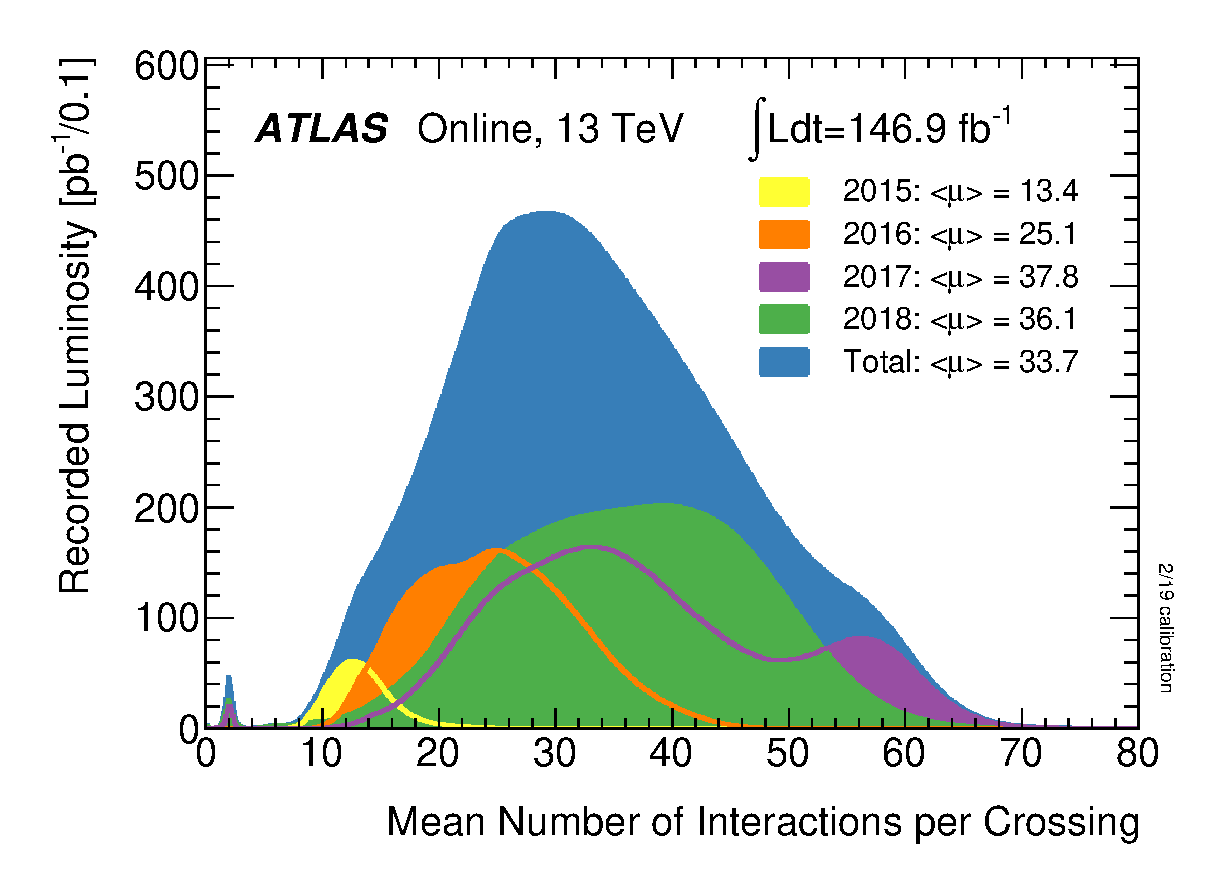
\includegraphics[width=0.55\linewidth]{Pictures/mu_2015_2018.eps}
    \caption{The luminosity-weighted distribution of the mean number of interactions per crossing is shown for Run 2 $pp$ collision data~\cite{lumigroup}. }
    \label{fig:mu_profile}
\end{figure}

Events are only used if all relevant detector components are operating normally. These events are part of the standard ``All Good'' Good Run List comprising a total integrated luminosity of $139$ fb$^{-1}$ and data quality efficiency of $91.5$\%.

Throughout Run 2, the instantaneous luminosity and pile-up changed over time. This is accounted for in our MC modeling, as described in the next section.

%%%%%%%%%%%%%%%%%%%%%%%%%%%%%%%%%%%%
\subsection{Monte Carlo samples}

Monte Carlo samples are generated to compare to data in order to test Standard Model predictions and search for discrepancies. These simulations are also used to optimize the analysis selection criteria. Monte Carlo events are fully simulated using the ATLAS detector simulation in the GEANT4 framework~\cite{GEANT4} and reconstructed with standard ATLAS reconstruction software. Pile-up is simulated as additional $pp$ interations in a separate simulation step during digitization where minimum bias events are superimposed on the simulated signal events. These additional events are added based on that year's recorded pile-up to account for dataset differences. 

Separate programs are used to generate the hard scattering process and to model the parton showering (PS), hadronization, and the underlying event (UE). The next sections summarize the simulation techniques for our signal VBF samples, other Higgs production modes, and relevant backgrounds.   

The data is split into three time-based categories. Data-taking conditions in 2015 and 2016 are averaged and described together as MC16a. The 2017 and 2018 data-taking conditions are considered separately as MC16d and MC16e, respectively. 

%%%%%%%%%%%%%%%%%%%%%%%%%%%%%%%%%%%%%%%%%%%%%%%%%%%%%%
\subsubsection{Vector boson fusion Higgs samples}

VBF Higgs events are generated through \textsc{POWHEG}~\cite{Nason:2009ai} interfaced with \textsc{Pythia8} with the PDF4LHC15 parton distribution function (PDF) set~\cite{PDF4LHC15}. Cross-sections are calculated with full NLO QCD and EW corrections~\cite{Ciccolini:2007jr, Arnold:2008rz} with an approximate NNLO QCD correction applied~\cite{Bolzoni:2010xr}. These cross-sections as well as associated branching ratios are calculated by the LHC Higgs Cross Section Working Group Yellow Report 4~\cite{LHCCrossSectionWG}. Generated events are normalized to the calculated cross-sections. 
%%%%%%%%%%%%%%%%%%%%%%%%%%%%%%%%%%%%%%%%%%%%%%%%%%%%%%
\subsubsection{Other production mode Higgs samples}

Other Higgs production modes are considered in the analysis including gluon fusion (ggF), associated Higgs boson production ($VH$, $V=W,Z$), and Higgs boson production in association with a heavy quark pair ($ttH$). Though only ggF has an appreciable yield in the signal region, each of these are studied and considered in the analysis. As in VBF Higgs sample, ggF, $VH$, and $ttH$ are produced with \textsc{Pythia8}~\cite{pythia,Sjostrand:2007gs} for decay, parton shower, hadronization and multiple parton interactions.
 
%%%%%%%%%%%%%%%%%%%%%%%%%%%%%%%%%%%%%%%
\subsubsection{Background samples}
\label{sec:bkgMC}

Standard Model backgrounds include events from production of dibosons, top-quark, $Z$+jets, $W$+jets and multijets. The $WW$ samples are generated using \textsc{SHERPA} 2.2.2 interfaced with NNPDF3.0 NNLO PDFs. The production of $Z$+jets (or Drell-Yan) is simulated with \textsc{SHERPA} 2.2.1 using the NNPDF3.0 NNLO PDFs with dedicated parton shower tuning developed by Sherpa authors. Top-quark pair production ($t\bar{t}$) is simulated using \textsc{POWHEG} with the \textsc{Powheg-Box} framework using the NNPDF 3.0 PDFs and interfaced with \textsc{Pythia 8} using NNPDF 2.3 PDFs for parton showering. Single top, mainly $Wt$, production is generated with \textsc{Powheg-Box} 2.0 interfaced to \textsc{Pythia} 6.428 for parton showering. The productions of $Z\gamma$ and $W\gamma$ are modeled using \textsc{SHERPA} 2.2.2 at the NLO accuracy for 0- and 1-jet. The $W$+jets process modeling is based on a data-driven method described in the next chapter. MC samples (with the same MC generators for both $W+$jets and $Z+$jets samples) are used to validate the fake estimation and estimate sample composition uncertainties. These processes are generated with \textsc{POWHEG} MiNLO interfaced to \textsc{Pythia 8} with the AZNLO tune. 

\section{Object definitions}
This analysis utilizes a number of calibrated physics objects and the accurate use of each determines the precision of our $H\rightarrow WW$ cross-section measurement. Lepton, jet, and missing transverse energy reconstruction, isolation, and calibration were described in the Chapter 4. This chapter focuses on the particular parameters applied for these physics objects in this analysis. The object definitions are used in accordance with the $H\rightarrow WW$ coupling analysis for consistency where optimization focussed on $H \rightarrow WW$ measurements at large. Finally, further observables used in event selection are defined and described here as well. 

\subsection{Lepton}

Our choice of lepton identification algorithm impacts both the rejection of fake lepton backgrounds ($W+$jets) and QCD background. Tighter requirements on lepton identification decrease signal efficiency so the optimal criteria balance high signal efficiency and high background rejection.

Overall, all events must have at least two leptons tracks and each lepton track must have $p_T>400$ MeV. Further, leptons are all required to originate at the hard-scatter primary vertex, which is defined as the primary vertex with the largest track $\sum p_T^2$. Leptons must pass two impact parameter selections to ensure they originate at the primary vertex. The longitudinal impact parameter of each lepton track is defined as $|z_0\mathrm{sin}\theta|$ where $z_0$ is the impact paramter and $\theta$ the track angle. Each lepton longitudinal impact parameter must be less than 0.5 mm. The significance of the transverse impact parameter is calculated with respect to the beam line ($|d_0|/\sigma_{d_0}$) and has a requirement of three (five) for muons (electrons), as recommended by the Muon and E/$\gamma$ combined performance groups. 

\subsubsection{Electron}
This analysis uses both the \textit{Medium} and \textit{Tight} identification selections which have 94\% and 88\% identification efficiency, respectively, for an electron with $E_T=100$  GeV. Electrons with $E_T>25$ GeV must pass the \textit{Medium} identification while those with $15<E_T<25$ GeV are required to pass the \textit{Tight} selection. This selection is the same used in the $H\rightarrow WW$ coupling analysis where optimization studies demonstrated its impact on overall significance. 

Electrons are identified in the range $|\eta|<2.47$, where the transition region between barrel and endcaps in the LAr calorimeter ($1.37<|\eta|<1.52$) is excluded.

Electron isolation uses two different selections based on electron track $p_T$. The \textit{IsoGradient} working point is used for $p_T>25$ GeV. This requires calorimeter and track isolation about cones of $\Delta R =0.2$ (\textit{topoetcone20}, \textit{ptvarcone20}). Electron isolation is changed to the fixed cut track cone isolation for $p_T <25$ GeV to further eliminate fake background contributions. These require both track and calorimeter variables to fall below the $p_T$ dependent $0.1143\times p_T + 92.14$. 

Table~\ref{tab:ElecSelection} summarizes electron selection criteria.

\begin{table}[h!]
  \centering
  \caption{Electron selections}
  \resizebox{\textwidth}{!}{
  \begin{tabular}{llccll}
    \hline\hline
     $p_T$ range & $|\eta|$ range   & Electron ID & Isolation     & Impact parameter\\
    \hline\hline
      $< 25$ GeV & \multirow{2}{*}{$0 - 1.37$, $1.52 - 2.47$}  & Tight           & FixedCutTrackCone40 & \multirow{2}{*}{$|z_0 \mathrm{ sin} \theta|<0.5$, $|d_0|/\sigma_{d_0}<5$} \\
      $> 25$ GeV &                                                              & Medium          & IsoGradient            & \\
    \hline\hline 
  \end{tabular}}
  \label{tab:ElecSelection}
\end{table}

\subsubsection{Muon}

As described previously, muons can be reconstructed using inner detector tracks, calorimeter deposits, and muon spectrometer tracks. Muons in this analysis must fit the \textit{Tight} selection as well as pass $p_T>15$ GeV and $|\eta|<2.5$. Muon identification and isolation criteria match those used in the $H\rightarrow WW$ coupling analysis and optimize background rejection and signal efficiency. Muon isolation uses calorimeter and track isolation with a cone of $\Delta R=0.2$ (\textit{topoetcone20, ptvarcone20}). 
Muon selection criteria are summarized in Table~\ref{tab:MuonSelection}. 

\begin{table}[h]
  \centering
  \caption{Muon selections}
  \resizebox{\textwidth}{!}{
  \begin{tabular}{llrccc}
    \hline\hline
     $p_T$ range   & $|\eta|$ range & Muon ID    & Calo Isolation           & Track Isolation             & Impact parameter\\
    \hline\hline
      $> 15$ GeV & $< 2.5$  & Tight  & $E_T^{cone20}/p_T<0.09$  & $p_T^{varcone30}/p_T<0.06$  & $|z_0 \mathrm{ sin} \theta|<0.5$, $|d_0|/\sigma_{d_0}<3$ \\
    \hline\hline
  \end{tabular}}
  \label{tab:MuonSelection}
\end{table}


%%%%%%%%%%%%%%%%%%%%%%%%%%%%%%%%%%
\subsection{Jets}

Jets constitute an important part of the analysis both in their number and characteristics. Our signal region selection and most control regions require at least two jets. In order to estimate and reject $ggF$ Higgs background events, regions with less than two jets are also studied. ``Tagging'' jets refer to those considered in our jet requirement, though others may be defined. As detailed in Section 4.4, jets reconstruction uses the anti-$k_t$ algorithm to create jet tracks from calorimeter deposited energy within a cone of $R = 0.4$, and this analysis uses particle flow jet reconstruction.   

Jets are required to have $p_T > 30$ GeV to eliminate high potential for pile-up jets in the full $\eta$ range, $|\eta| < 4.5$. ``Jet vertex tagger'' variables suppress pile-up events through combinations of multiple variables into a single jet tagger. For jets with $p_T < 60$ GeV and $|\eta| < 2.4$, the JVT variable is required to be larger than 0.59. In the forward region, a designated tagger called ``fJVT'' ought to be applied. However, the current analysis does not include this requirement, leading to more jet pile-up than expected. 

The VBF signal region contains an additional jet observable, the central jet veto (CJV), which rejects events with additional jets (other than the two ``tagged'' jets) with $p_T>20$~GeV within the rapidity gap between two leading jets. This veto increases VBF sensitivity through removal of hadronic backgrounds.
%%%%%%%%
\subsubsection{$b$-tagged jet}

The Jet/$E_T^{miss}$ group provides tools to identify jets formed from bottom quarks. While the previous HWW analysis~\cite{Aaboud_2019} used the MV2C10 jet tagging algorithm, the current analysis utilizes the DL1 tagger. Both tools use jet kinematics, impact parameters, and secondary vertex variables as input to machine learning classifiers. The DL1 tagger uses a neural network training method (the MV2C10 a boosted decision tree) trained with $t\bar{t}$ signal to discriminate $b$-quarks from light and $c$-quarks. The DL1 tagger shows greater $b$-veto efficiency in isolating top background events and so is used in this analysis. 

%%%%%%%%%%%%%%%%%%%%%%%%%%%%%%%%%
\subsection{Missing transverse energy}

Missing transverse energy is used to both suppress background and build other variables used in signal selection like $m_{tt}$ and $p_T^{tot}$. The $E_T^{miss}$ definitions and calculations are explained in Section 4.5. This analysis uses the ``Tight'' $E_T^{miss}$ working point which has proven the most robust against increasing pile-up.

%%%%%%%%%%%%%%%%%%%%%%%%%%%%%%%%%
\subsection{Overlap removal}
Overlap removal is applied to electrons, muons, and jets following the latest algorithm recommended by the Analysis Software Group (ASG). Current removal steps can be summarized as followed:
\begin{itemize}
\item If a muon and electron share an ID track the electron is removed and if a calo-tagged muon shares an ID track with an electron, the muon is removed.
\item If $\Delta R$(jet, $e$) $< 0.2$ the jet is removed to eliminate overlap with the nearby electron. The electron is removed if $\Delta R$ (jet, $e$) $<$ min(0.4, 0.04 + 10 GeV/$p_T^e$).
\item If $\Delta R$ (jet, $\mu$) $< 0.2$ and the jet has less than three associated tracks with $p_T>500$ MeV the jet is removed. The jet is also removed if the $p_T$ ratio of the muon and jet is larger than 0.5 and the ratio of the muon $p_T$ and the sum of the $p_T$ of all jet tracks with $p_T>500$ GeV is larger than 0.7. The muon is removed if $\Delta R$(jet, $\mu$) $<$ min(0.4, 0.04 + 10 GeV/$p_\mathrm{{T}}^{\mu}$) for any surviving jets.
%\item Jets are discarded if they are within a cone of size $\Delta R < 0.2$ of an electron candidate, or if they have less than three associated tracks and are within a cone of size $\Delta R < 0.2$ of a muon candidate. However, if a jet with three or more associated tracks is within a cone of size $\Delta R < 0.4$ of a muon candidate, or any jet is within $0.2 < \Delta R < 0.4$ of an electron candidate, the corresponding electron or muon candidate is discarded. 
\end{itemize}


%%%%%%%%%%%%%%%%%%%%%%%%%%%%%%%%%%%%%%%%%%%%%%%%
\section{Common Observables}

Dedicated observables are used in this analysis to reject and isolate backgrounds as well as to enhance VBF signal strength. This section lists and describe key observables used in the analysis.

\begin{itemize}
\item $m_{\tau \tau}$: This is fully defined in Section 4.5. If charged leptons are the products of a pair of $\tau$ leptons, the neutrinos are assumed to be collinear with the charged leptons, and the neutrinos are the only source of the observed $E_\mathrm{{T}}^{miss}$. Requirements on this variable target $Z\rightarrow \tau\tau$ events. 
\item $N_{b-jet}$: Defines the number of jets with $p_T >20$ GeV identified as $b$-jets from the $b$-tagging algorithm (DL1) and is used to reject $t\bar{t}$ background.
%\item $p_\mathrm{{T}}^{ll}$: The transverse momentum of the dilepton system. This cut targets Drell-Yan/$Z\rightarrow\tau\tau$ events requiring $p_{\text{T}}^{ll}>$ GeV. 
\item $\Delta \phi_{ll}$: The two leptons from HWW decays tend to be collimated especially compared to non-resonant WW backgrounds. This is due to the spin-zero initial state of the resonant process. 
\item $m_{ll}$: The invariant mass of the two leptons from the hard scattering interaction; this targets Drell-Yan events and requires $m_{ll}>70$ GeV in the control region.
\item $m_\mathrm{{T}}$: Transverse mass is used as a discriminant for the $Z+$jets control region. It is defined as
\begin{equation}
m_\mathrm{{T}} = \sqrt{ {(E_{ll} + E_\mathrm{{T}}^{miss})}^2 - {|p_{ll} + E_\mathrm{{T}}^{miss}|}^2 },
\end{equation}
  where $E_{ll} = \sqrt{|p_{ll}|^2 + m_{ll}^2 }$ .
\item $p_T^\mathrm{tot}$:
Total transverse momentum $p_T^\mathrm{tot}$ is defined in Section 4.5. This variable isolates events with significant soft gluon radiation but not high $p_T$ jets.
\item  $\Delta Y_{jj}$: VBF Higgs signal events are characterized by a large separation of the two tagging jets in rapidity. This variable is used as a signal region cut. 
\item $m_{jj}$:
VBF Higgs events end to have a high jet invariant mass ($m_{jj}$), defined by combining mass of tagged jets. This analysis applies a cut on $m_{jj}$ in our signal region. 
\item $\eta_{lep}$ centrality: This analysis uses an outside lepton veto defined to reject events with leptons outside the rapidity gap between the two tagged jets. The sum of the centralities of each lepton is used as a discriminant to train various multivariate classifiers. The OLV variable is defined using pseudorapidity of the tagged jets and leptons as follows:
\begin{eqnarray}
&& \textrm{OLV}_{l_0} = 2 \cdot |\frac{\eta_{l_0}-\bar{\eta}}{\eta_{j_0}-\eta_{j_1}}|,  \nonumber\\
&& \textrm{OLV}_{l_1} = 2 \cdot |\frac{\eta_{l_1}-\bar{\eta}}{\eta_{j_0}-\eta_{j_1}}|,  \nonumber\\
&&\nonumber \\
&& \eta_{\mathrm{lep}} \, \textrm{centrality} = \textrm{OLV}_{l_0} + \textrm{OLV}_{l_1},
\label{eqn:contOLV_def}
\end{eqnarray}
where $\bar{\eta} = (\eta_{j_0} + \eta_{j_1})/2$ and so for each lepton: 
 \begin{equation}
   \textrm{OLV}_l \left\{
   \begin{array} {ll}
     = 0 & \quad \rightarrow \textrm{  The lepton is within the rapidity gap between the two tagged jets.} \\
     < 1 & \quad \rightarrow \textrm{  The lepton lies within the rapidity gap between the two tagged jets.} \\
     >1  & \quad \rightarrow \textrm{   The lepton is outside the rapidity gap between the two tagged jets.} 
    \end{array} \right. 
 \end{equation}
\item $\mathrm{\sum_{l,j} M_{lj}}$: The sum of the invariant masses of all possible lepton-jet pairs are used to train our signal discriminant as VBF Higgs signal peaks at a higher value than the dominant backgrounds. VBF signal jets tend to be very forward while lepton central so a large separation between lepton and jets is expected as opposed to typical background topologies. 
\end{itemize}


\section{Event selection}
Figure~\ref{fig:FeynmanDiagramVBF} shows the Feynman diagram for the vector boson fusion Higgs production mode. Two energetic jets with large separation in rapidity accompany the Higgs and its decay products. In addition, since the Higgs is created through the fusion of two electro-weak bosons, there is no QCD interaction between the jets and the Higgs boson or its decay products. The main backgrounds this analysis seeks to mitigate include top quark production, Drell-Yan/$Z$, di-bosons ($WW$, $WZ$, $ZZ$, and $W\gamma$), ggF Higgs production, and $W$+jets. 

\begin{figure}[!htbp]
    \centering
    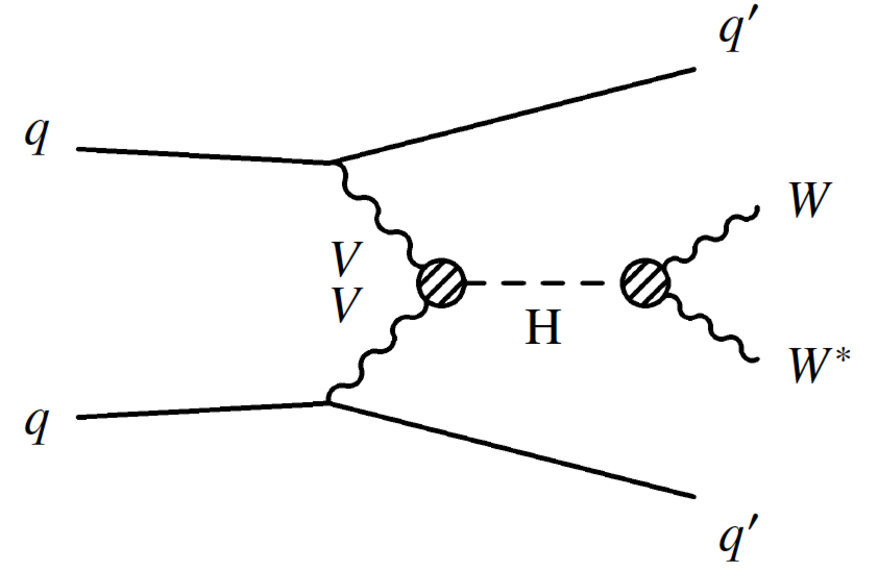
\includegraphics[width=0.4\linewidth]{Pictures/fig_01b_2.pdf}
    \caption{Feynman diagram for VBF Higgs production~\cite{Djouadi}}
    \label{fig:FeynmanDiagramVBF}
\end{figure}

This analysis controls and estimates these backgrounds with a variety of methods depending on the characteristics of each background. Major backgrounds are estimated in CRs and minor backgrounds are estimated using MC simuation. Top quark production is suppressed in the SR by a $b$-jet veto requirement and can be studied in a very pure orthogonal set of bins in the signal region defined by a boosted decision tree discriminant. A pure validation region is also defined to cross-check top MC modeling. The Drell-Yan/$Z$ background is suppressed by kinematic requirements and is constrained in a dedicated and orthogonal CR and ultimately normalized in the signal phase space. The $ggF$ Higgs produciton mode is particularly difficult to separate from the VBF production mode, therefore several CRs are defined to constrain it in data, and ultimately its normalization is determined in the signal phase space. Other Higgs production modes ($VH$ and $ttH$) are analyzed and included as backgrounds, but play a very small role in our overall result. The $W$+jets background is estimated with data-driven techniques, as described in the Chapter 6, and then fixed in the simultaneous fit of SR and CRs.

We utilize multivariate analysis (MVA), more specifically gradient boosted decision trees trained to discriminate between samples. There are six trained BDTs used to separate $WW+$top and $VBF$ events, $VBF$ and ggF events, ggF events from all other samples in each of their three control regions, and $WW+$top events and all other samples. The use of these BDTs separates the backgrounds from our signal in the signal region and maintains discrimination between the $WW$ and top background samples. 

The $WW+$top vs. VBF BDT is discussed in this chapter while the others are explained with their associated backgrounds in Chapter 6. In addition, two other types of BDT have been tested in this analysis: a $Z+$jets vs. VBF BDT and a 3D BDT to separate $ggF$, $WW$ and VBF events. Results from these tests showed that though these led to minimization of background (in the case of $Z+$jets vs. VBF) and good discrimination between key backgrounds in the signal region (in the case of the 3D BDT), when used in the final fit with systematic uncertainties they showed no significant decrease in calculated error in the VBF coupling value. Results from these studies are shown in Appendix B and C.

\begin{table}[h!]
\centering
\resizebox{\textwidth}{!}{
\begin{tabular}{|l|c|c|c|c|c|}
\hline
\multirow{2}{*}{Background}   & Relative size  & Relative size  & \multirow{2}{*}{Estimation}  & \multirow{2}{*}{{Generator}} \\
                              & Pre-selection  & Signal Region  &                       & \\
\hline                                                         
$WW$                       & $\sim 8\%$               & $\sim20\%$    & MC only + BDT           & \textsc{SHERPA} 2.2.2 ($gg \rightarrow WW$: \textsc{SHERPA} 2.1)\\
Top		              & $\sim 73\%$   	       &  $\sim61\%$     & MC only + BDT       & \textsc{POWHEG}+\textsc{Pythia} 8\\
$ggF$ Higgs                     & $< 1\%$    	       &  $\sim2\%$     & MC only + BDT           & \textsc{POWHEG}+\textsc{Pythia} 8 NNLOPS\\
$W$+jets                        & $\sim2.5\%$ 		& $\sim4\%$ 	& Data-driven           & - \\
$Z\rightarrow \tau\tau$                          & $\sim16\%$	       & $\sim7\%$		& Data+MC ($Z\rightarrow \tau\tau$ CR)     & \textsc{SHERPA} 2.2.1 \\
$W\gamma$,$W\gamma^{*}$       & $\sim1\%$		&  $\sim2.5\%$    & MC only               & \textsc{SHERPA} 2.1/\textsc{SHERPA} 2.2.2 \\
\hline
\end{tabular}
}
\caption{Each background and its relative size of in SR (after all cuts), estimation method, and generator.}
\label{tab:bkgsum}
\end{table}

\subsection{Pre-selection}
The VBF differential analysis shares object definitions with the VBF and ggF coupling analysis and pre-selection cuts are based off of those used in the 2016 ggF and VBF $H\rightarrow WW$ 36.1 fb$^{-1}$ cross-section paper~\cite{Aaboud_2019}. The VBF selection utilizes observables defined in the previous section. Cuts applied in the preselection region are listed and described in Table~\ref{tab:preseldef}. 
\begin{table}[h!]
\centering
\resizebox{\textwidth}{!}{
\begin{tabular}{|l|c|c|c|c|c|}
\hline
\multirow{2}{*}{Pre-sel cut}   & Description \\
				&	 \\
\hline
Channel Selection	& Fits $e\mu$/$\mu e$ channel/event weight applied\\  
Trigger Selection	&  Trigger selected \\
Trigger Matching	&  Trigger weight applied  \\
Data driven muon/electron & W+jets split into electron and muon fake flavors \\
Cut Jet Cleaning	& Pass loose jet cleaning \\
Cut $V\gamma$/$Z+$jets overlap & Eliminate any $Z+$jets events that overlap with $V\gamma$ \\ 
Only two leptons       	&  Require exactly 2 leptons (in case of fakes make sure 1 ID/1 Anti-ID) \\
Lead lepton $p_T$	& $p_T^{lead} > 22 $GeV \\
Sublead lepton $p_T$	& $p_T^{sublead} >15 $GeV \\
Opposite sign leptons	&  Require zero dilepton charge \\
Fake Factor	& W+jets weight applied \\
\hline
\end{tabular}}
\caption{Table describing pre-selection cuts applied in common with VBF and $ggF$ coupling analyses}
\label{tab:preseldef}
\end{table}

Yields for all samples as well as data for pre-selection cuts are shown in Table~\ref{tab:preselcut}.
\begin{table}[h!]
\resizebox{\textwidth}{!}{
%%% created on Sat Apr 18 17:21:56 2020 from TQSampleFolder 'samples' with TQLibrary UNKNOWN compiled with GCC 8.3.0 against ROOT 6.16/00
\providecommand{\xmark}{{\sffamily \bfseries X}}
\providecommand\rotatecell[2]{\rotatebox[origin=c]{#1}{#2}}
\begin{tabular}{ r || r  r | r  r || r  r  r | r  r  r  r }
\ensuremath{\sqrt{s}=13 TeV}, \ensuremath{\mathcal{L}=139 fb^{-1}}  (Full~Run~2) & $H_{VBF}$ & $H_{ggF}$ & $WW$ & Other VV & Top & Zjets & Mis-Id & Total Bkg & Significance & Data & Data/MC\tabularnewline
\hline
Channel Selection & \ensuremath{904.81\pm 0.92} & \ensuremath{9240.38\pm 10.13} & \ensuremath{175857.28\pm 140.42} & \ensuremath{22386.99\pm 78.25} & \ensuremath{1709307.70\pm 287.98} & \ensuremath{655027.79\pm 1233.45} & \ensuremath{5008168.16\pm 4730.67} & \ensuremath{7579988.31\pm 4899.95} & \ensuremath{0.33\pm 0.00} & \ensuremath{4374979} & \ensuremath{0.58\pm 0.00}\tabularnewline
Trigger Selection & \ensuremath{904.81\pm 0.92} & \ensuremath{9240.38\pm 10.13} & \ensuremath{175857.28\pm 140.42} & \ensuremath{22386.99\pm 78.25} & \ensuremath{1709307.70\pm 287.98} & \ensuremath{655027.79\pm 1233.45} & \ensuremath{5008168.16\pm 4730.67} & \ensuremath{7579988.31\pm 4899.95} & \ensuremath{0.33\pm 0.00} & \ensuremath{4374979} & \ensuremath{0.58\pm 0.00}\tabularnewline
Trigger Matching & \ensuremath{882.26\pm 0.90} & \ensuremath{8940.07\pm 9.82} & \ensuremath{173094.52\pm 138.41} & \ensuremath{21501.64\pm 77.38} & \ensuremath{1678206.02\pm 283.57} & \ensuremath{624251.33\pm 1168.16} & \ensuremath{5151805.35\pm 4644.01} & \ensuremath{7657798.93\pm 4799.69} & \ensuremath{0.32\pm 0.00} & \ensuremath{4352644} & \ensuremath{0.57\pm 0.00}\tabularnewline
W+jets flavour split muon & \ensuremath{882.26\pm 0.90} & \ensuremath{8940.07\pm 9.82} & \ensuremath{173094.52\pm 138.41} & \ensuremath{21501.64\pm 77.38} & \ensuremath{1678206.02\pm 283.57} & \ensuremath{624251.33\pm 1168.16} & \ensuremath{4675498.22\pm 4228.78} & \ensuremath{7181491.80\pm 4399.19} & \ensuremath{0.33\pm 0.00} & \ensuremath{4352644} & \ensuremath{0.61\pm 0.00}\tabularnewline
W+jets flavour split electron & \ensuremath{882.26\pm 0.90} & \ensuremath{8940.07\pm 9.82} & \ensuremath{173094.52\pm 138.41} & \ensuremath{21501.64\pm 77.38} & \ensuremath{1678206.02\pm 283.57} & \ensuremath{624251.33\pm 1168.16} & \ensuremath{3625576.16\pm 3693.41} & \ensuremath{6131569.74\pm 3887.35} & \ensuremath{0.36\pm 0.00} & \ensuremath{4352644} & \ensuremath{0.71\pm 0.00}\tabularnewline
Jet Cleaning & \ensuremath{882.26\pm 0.90} & \ensuremath{8940.07\pm 9.82} & \ensuremath{173094.52\pm 138.41} & \ensuremath{21501.64\pm 77.38} & \ensuremath{1678206.02\pm 283.57} & \ensuremath{624251.33\pm 1168.16} & \ensuremath{3625576.16\pm 3693.41} & \ensuremath{6131569.74\pm 3887.35} & \ensuremath{0.36\pm 0.00} & \ensuremath{4352644} & \ensuremath{0.71\pm 0.00}\tabularnewline
Overlap: Vgamma/Vjets & \ensuremath{882.26\pm 0.90} & \ensuremath{8940.07\pm 9.82} & \ensuremath{173094.52\pm 138.41} & \ensuremath{21501.64\pm 77.38} & \ensuremath{1678206.02\pm 283.57} & \ensuremath{624251.33\pm 1168.16} & \ensuremath{3625576.16\pm 3693.41} & \ensuremath{6131569.74\pm 3887.35} & \ensuremath{0.36\pm 0.00} & \ensuremath{4352644} & \ensuremath{0.71\pm 0.00}\tabularnewline
Only two Leptons & \ensuremath{880.17\pm 0.89} & \ensuremath{8934.45\pm 9.82} & \ensuremath{172870.71\pm 138.36} & \ensuremath{20467.40\pm 77.14} & \ensuremath{1662432.27\pm 282.33} & \ensuremath{622191.46\pm 1160.36} & \ensuremath{3621793.98\pm 3681.91} & \ensuremath{6108690.27\pm 3873.99} & \ensuremath{0.36\pm 0.00} & \ensuremath{4331979} & \ensuremath{0.71\pm 0.00}\tabularnewline
$p_{t}^{lead} > 22$ GeV & \ensuremath{880.17\pm 0.89} & \ensuremath{8934.45\pm 9.82} & \ensuremath{172870.71\pm 138.36} & \ensuremath{20467.40\pm 77.14} & \ensuremath{1662432.27\pm 282.33} & \ensuremath{622191.46\pm 1160.36} & \ensuremath{3621793.98\pm 3681.91} & \ensuremath{6108690.27\pm 3873.99} & \ensuremath{0.36\pm 0.00} & \ensuremath{4331979} & \ensuremath{0.71\pm 0.00}\tabularnewline
$p_{t}^{\rm sublead} > 15$ & \ensuremath{879.98\pm 0.89} & \ensuremath{8933.88\pm 9.82} & \ensuremath{172854.38\pm 138.35} & \ensuremath{20409.32\pm 77.10} & \ensuremath{1661877.68\pm 282.29} & \ensuremath{622068.28\pm 1160.19} & \ensuremath{3620023.39\pm 3681.17} & \ensuremath{6106166.94\pm 3873.23} & \ensuremath{0.36\pm 0.00} & \ensuremath{4330240} & \ensuremath{0.71\pm 0.00}\tabularnewline
OS Leptons & \ensuremath{879.86\pm 0.89} & \ensuremath{8933.68\pm 9.82} & \ensuremath{172771.82\pm 134.49} & \ensuremath{20042.40\pm 38.48} & \ensuremath{1661388.47\pm 282.25} & \ensuremath{621966.33\pm 1160.06} & \ensuremath{3614469.54\pm 3678.75} & \ensuremath{6099572.24\pm 3870.18} & \ensuremath{0.36\pm 0.00} & \ensuremath{4326784} & \ensuremath{0.71\pm 0.00}\tabularnewline
$M_{\ell\ell} > 12/10$ GeV & \ensuremath{879.85\pm 0.89} & \ensuremath{8933.66\pm 9.82} & \ensuremath{172771.33\pm 134.49} & \ensuremath{20041.83\pm 38.48} & \ensuremath{1661368.39\pm 282.25} & \ensuremath{621964.49\pm 1160.06} & \ensuremath{3614188.72\pm 3678.68} & \ensuremath{6099268.41\pm 3870.11} & \ensuremath{0.36\pm 0.00} & \ensuremath{4326642} & \ensuremath{0.71\pm 0.00}\tabularnewline
SF: Z Veto & \ensuremath{879.85\pm 0.89} & \ensuremath{8933.66\pm 9.82} & \ensuremath{172771.33\pm 134.49} & \ensuremath{20041.83\pm 38.48} & \ensuremath{1661368.39\pm 282.25} & \ensuremath{621964.49\pm 1160.06} & \ensuremath{3614188.72\pm 3678.68} & \ensuremath{6099268.41\pm 3870.11} & \ensuremath{0.36\pm 0.00} & \ensuremath{4326642} & \ensuremath{0.71\pm 0.00}\tabularnewline
Leptons ID, singleFakes 1 anti-ID,1 ID, doubleFakes 2*anti-ID & \ensuremath{596.53\pm 0.74} & \ensuremath{5630.33\pm 7.80} & \ensuremath{126996.63\pm 115.72} & \ensuremath{11152.41\pm 25.92} & \ensuremath{1165160.56\pm 237.51} & \ensuremath{257221.77\pm 444.61} & \ensuremath{1150777.06\pm 1622.64} & \ensuremath{2716938.76\pm 1703.28} & \ensuremath{0.36\pm 0.00} & \ensuremath{1587474} & \ensuremath{0.58\pm 0.00}\tabularnewline
Apply QCD FF weight & \ensuremath{596.53\pm 0.74} & \ensuremath{5630.33\pm 7.80} & \ensuremath{126996.63\pm 115.72} & \ensuremath{11152.41\pm 25.92} & \ensuremath{1165160.56\pm 237.51} & \ensuremath{257221.77\pm 444.61} & \ensuremath{523146.10\pm 1291.33} & \ensuremath{2089307.80\pm 1391.31} & \ensuremath{0.41\pm 0.00} & \ensuremath{1587474} & \ensuremath{0.76\pm 0.00}\tabularnewline
Apply fake factor & \ensuremath{596.53\pm 0.74} & \ensuremath{5630.33\pm 7.80} & \ensuremath{126996.63\pm 115.72} & \ensuremath{11152.41\pm 25.92} & \ensuremath{1165160.56\pm 237.51} & \ensuremath{257221.77\pm 444.61} & \ensuremath{36980.51\pm 255.27} & \ensuremath{1603142.22\pm 577.39} & \ensuremath{0.47\pm 0.00} & \ensuremath{1587474} & \ensuremath{0.99\pm 0.00}\tabularnewline
\hline
\end{tabular}

}
\caption{Cutflow in the pre-selection region.}
\label{tab:preselcut}
\end{table}

The plots in Figure~\ref{fig:preselection} show kinematic distributions after all preselection cuts with fake factors applied directly after a 2-jet cut. These show good modeling with data over a variety of kinematic variables including those used in the Top$+WW$ vs. VBF BDT. We were not able to directly examine modeling of input variables to this BDT because blinding is required in the signal region. Modeling in the pre-selection region was studied in lieu of this and showed no evidence of bias. In addition, normalization factors (NF) are calculated by data/MC comparisons in top ($Z\rightarrow\tau\tau$) validation (control) regions. These scale factors are added to $Z\rightarrow\tau\tau$ background events in order to correct for MC mis-modeling and are calculated to be $0.99\pm0.01$ and $1.01\pm0.04$, respectively. 

\begin{figure}[!h]
  \subfloat[$\Delta Y_{jj}$]{
      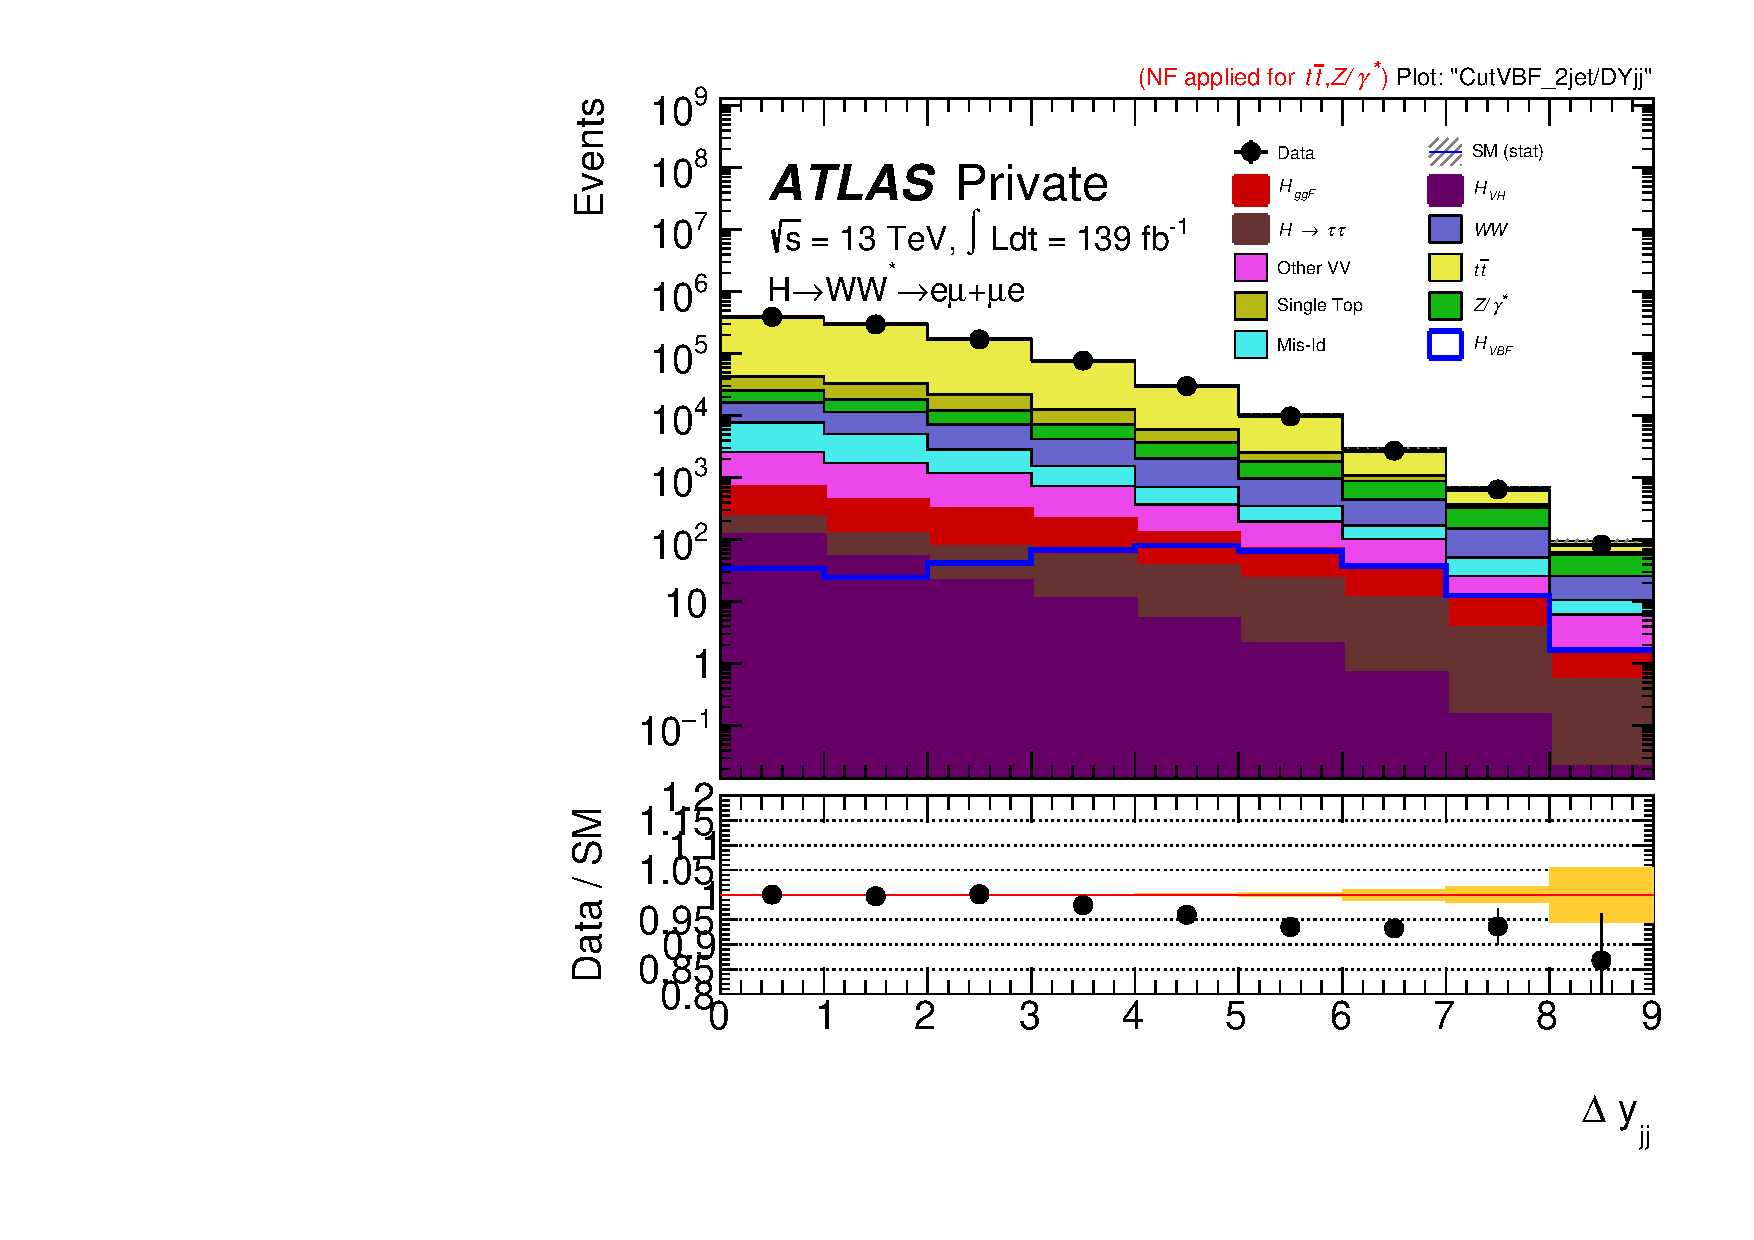
\includegraphics[width=0.3\textwidth]{Pictures/run2-emme-CutVBF_2jet-DYjj-log.pdf}
  }\hfill
  \subfloat[$\Delta Y_{\ell\ell}$]{
      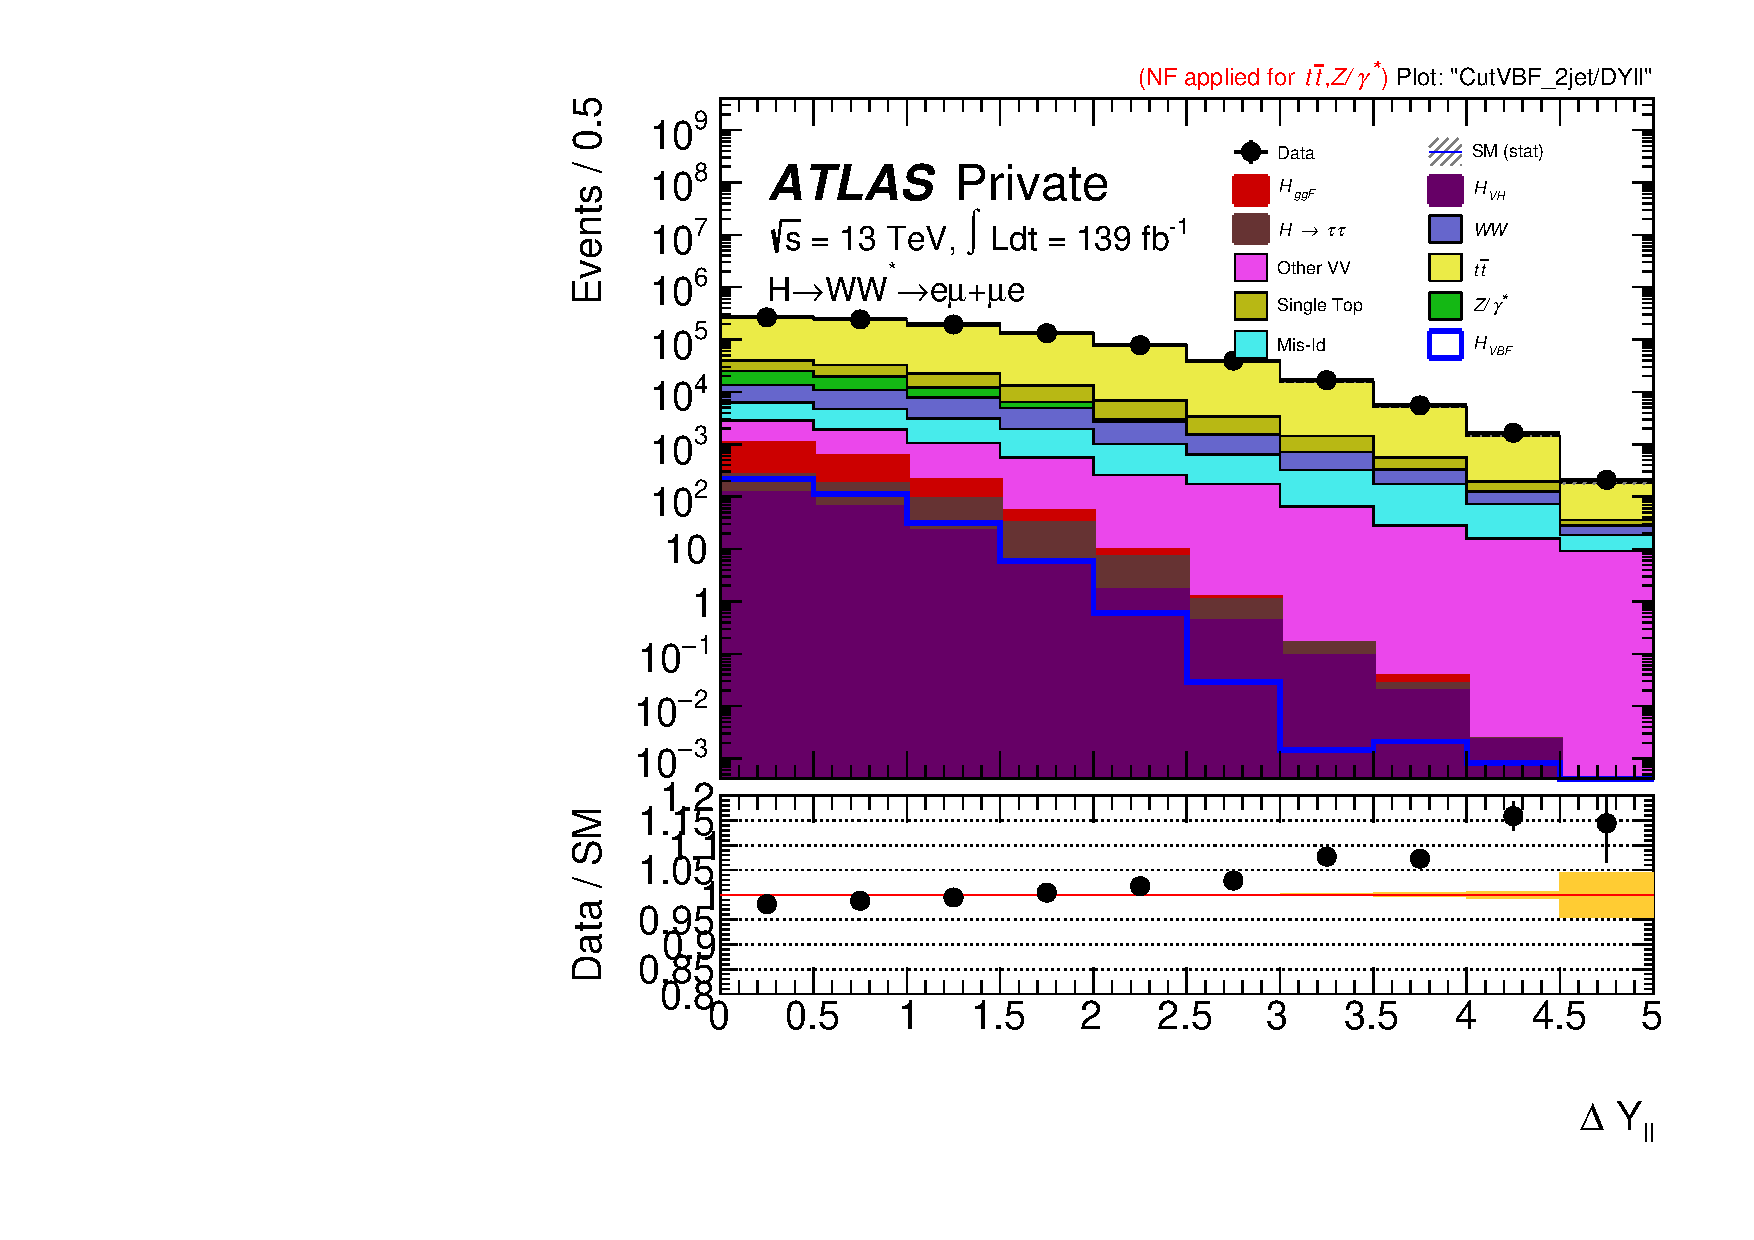
\includegraphics[width=0.3\textwidth]{Pictures/run2-emme-CutVBF_2jet-DYll-log.pdf}
  }\hfill
  \subfloat[$\Delta \phi_{\ell\ell}$]{
      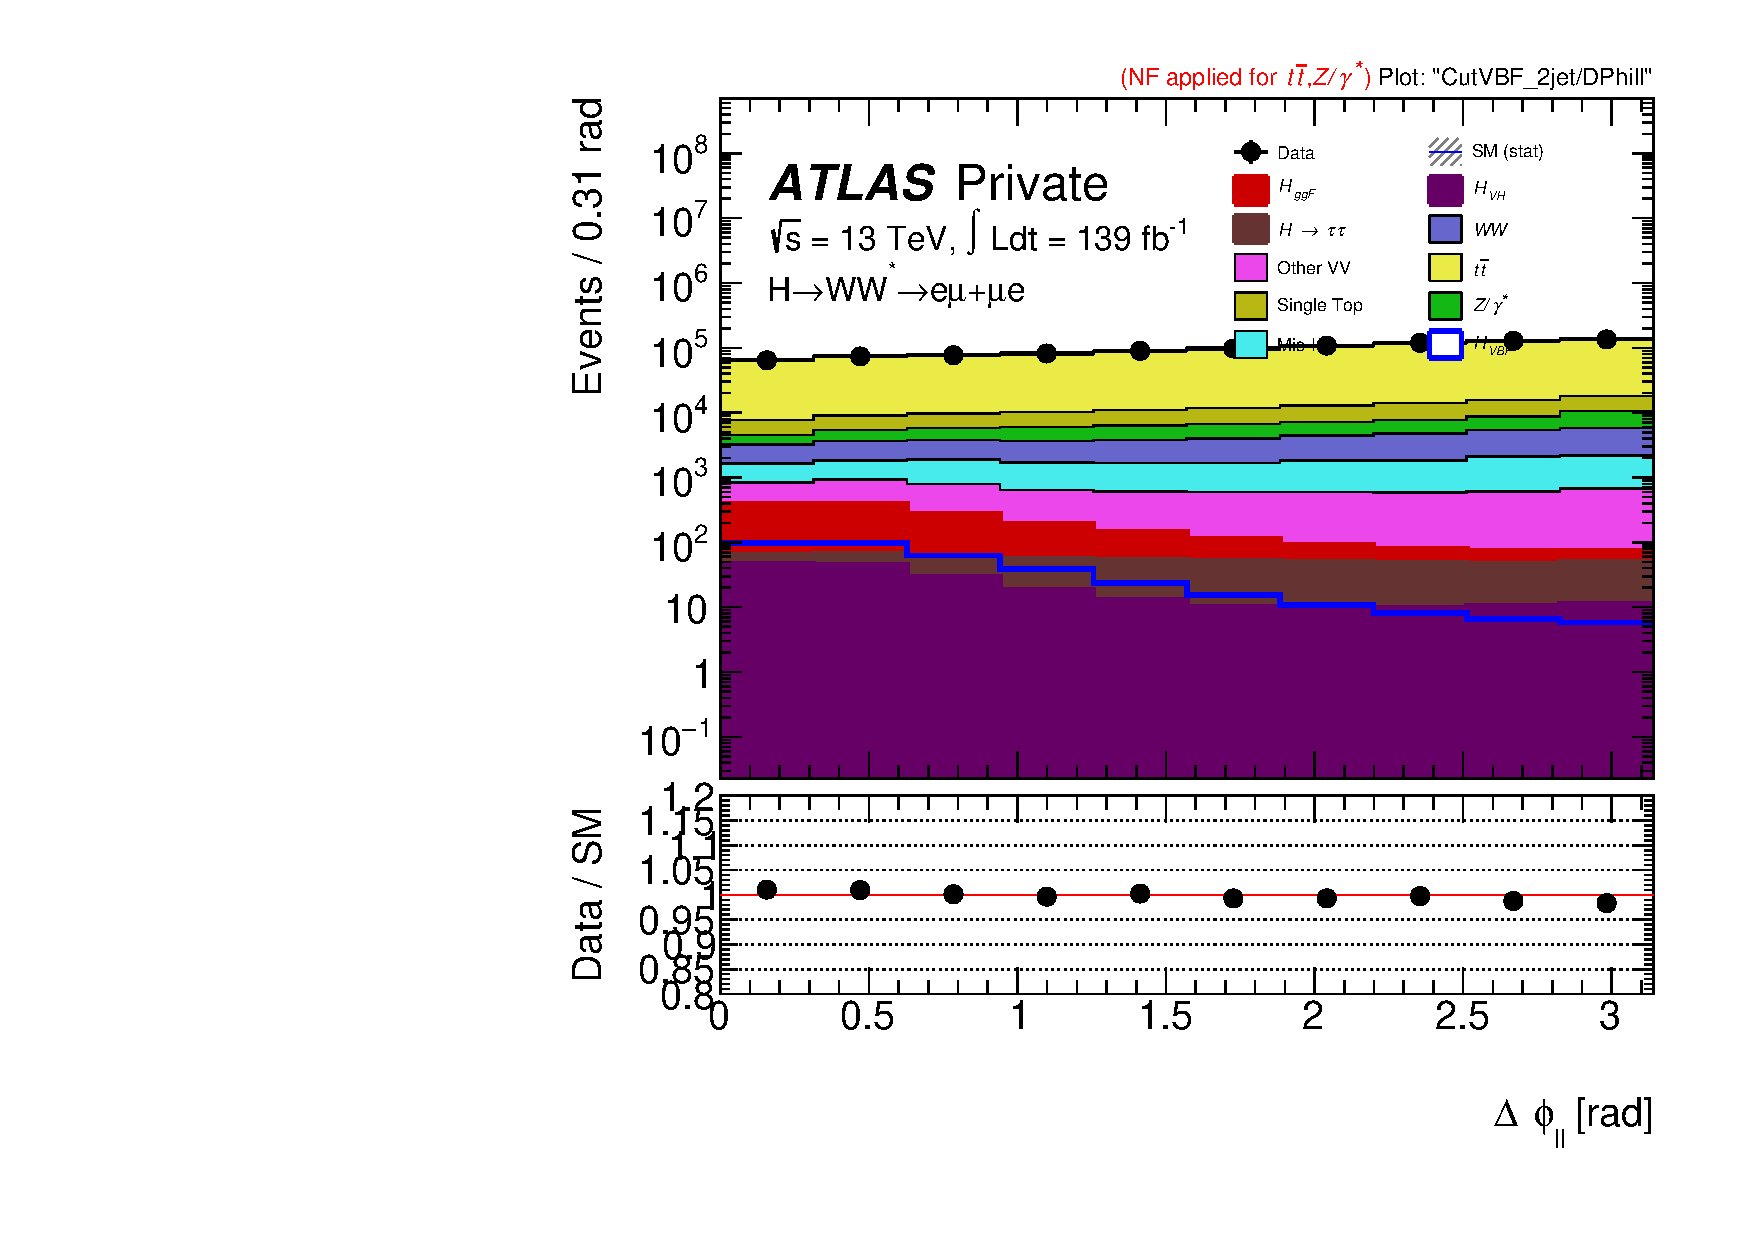
\includegraphics[width=0.3\textwidth]{Pictures/run2-emme-CutVBF_2jet-DPhill-log.pdf}
  }\hfill
  \subfloat[$m_{jj}$]{
      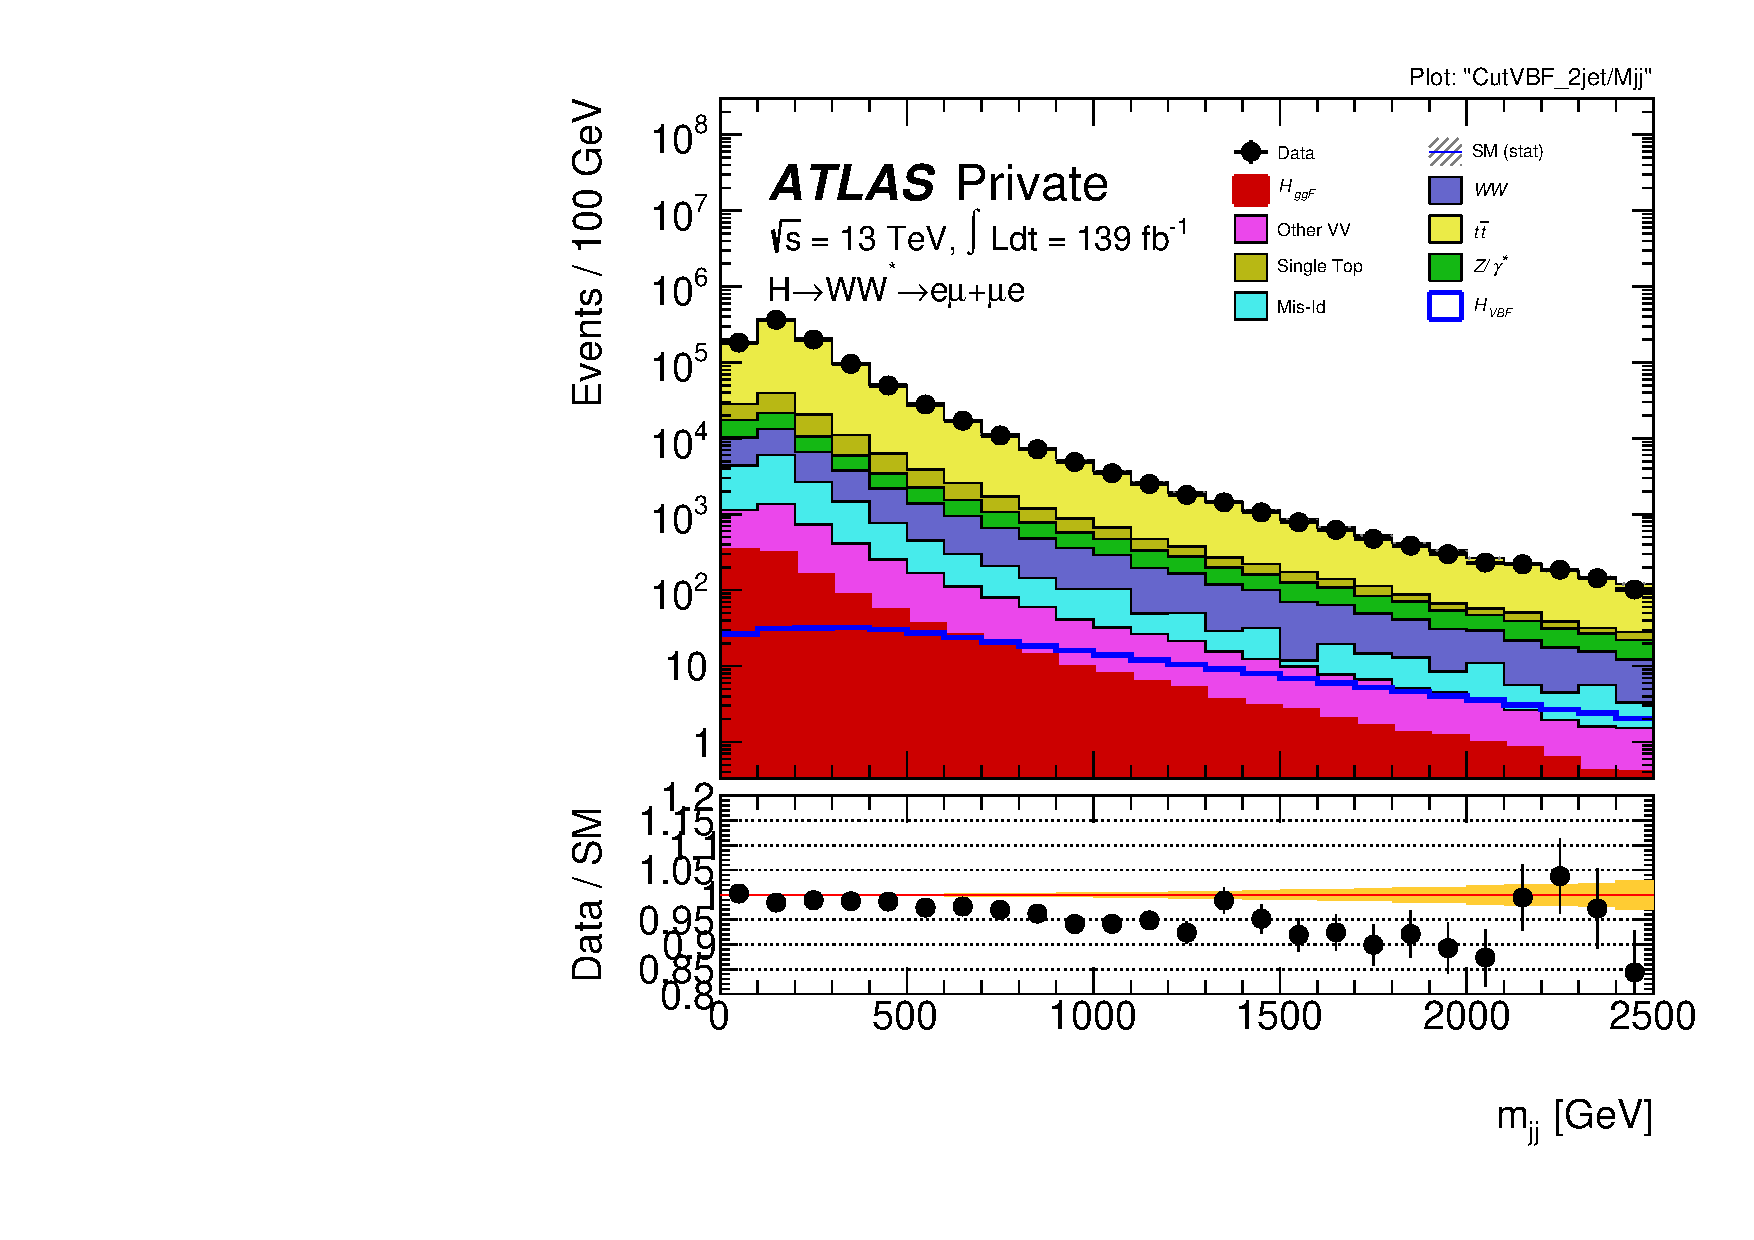
\includegraphics[width=0.3\textwidth]{Pictures/run2-emme-CutVBF_2jet-Mjj-log.pdf}
  }\hfill
  \subfloat[$m_{\ell\ell}$]{
      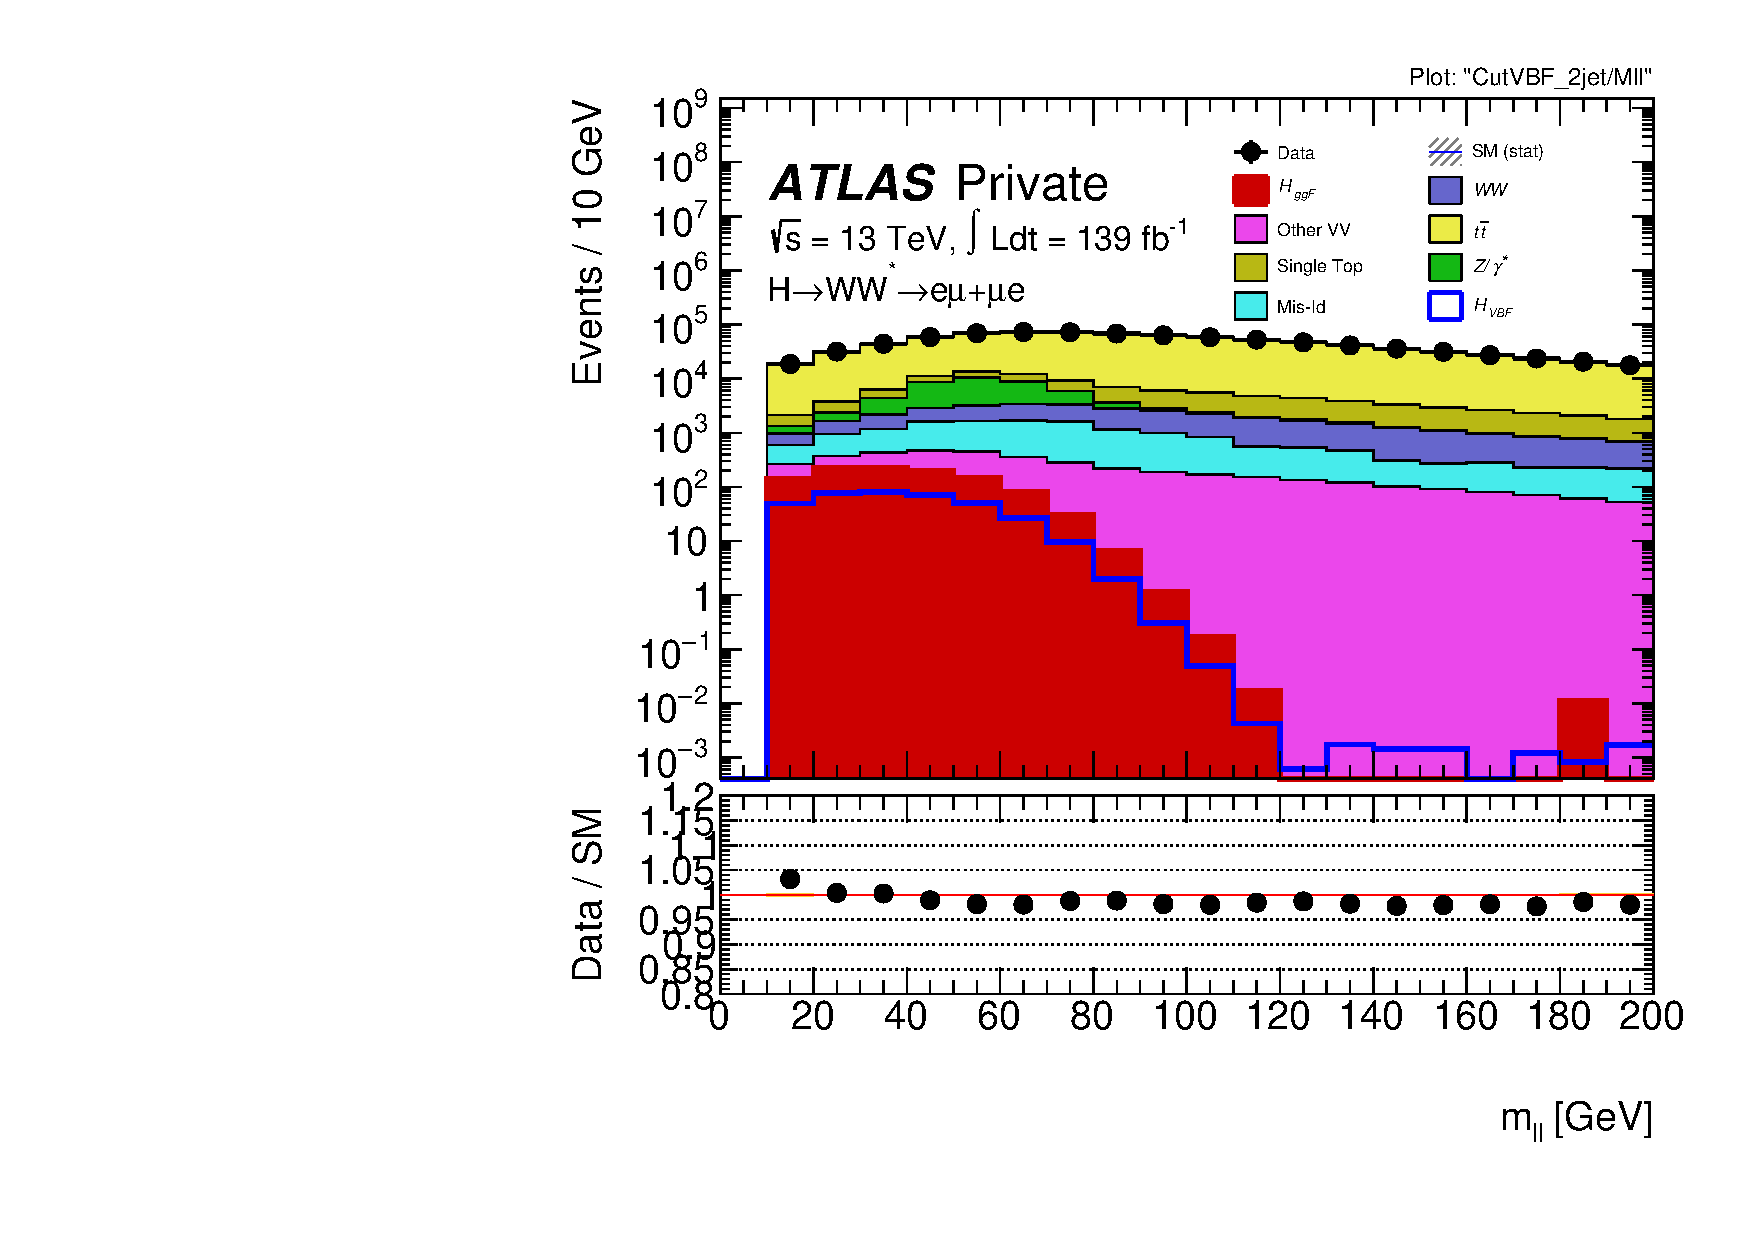
\includegraphics[width=0.3\textwidth]{Pictures/run2-emme-CutVBF_2jet-Mll-log.pdf}
  }\hfill
  \subfloat[$m_T$]{
      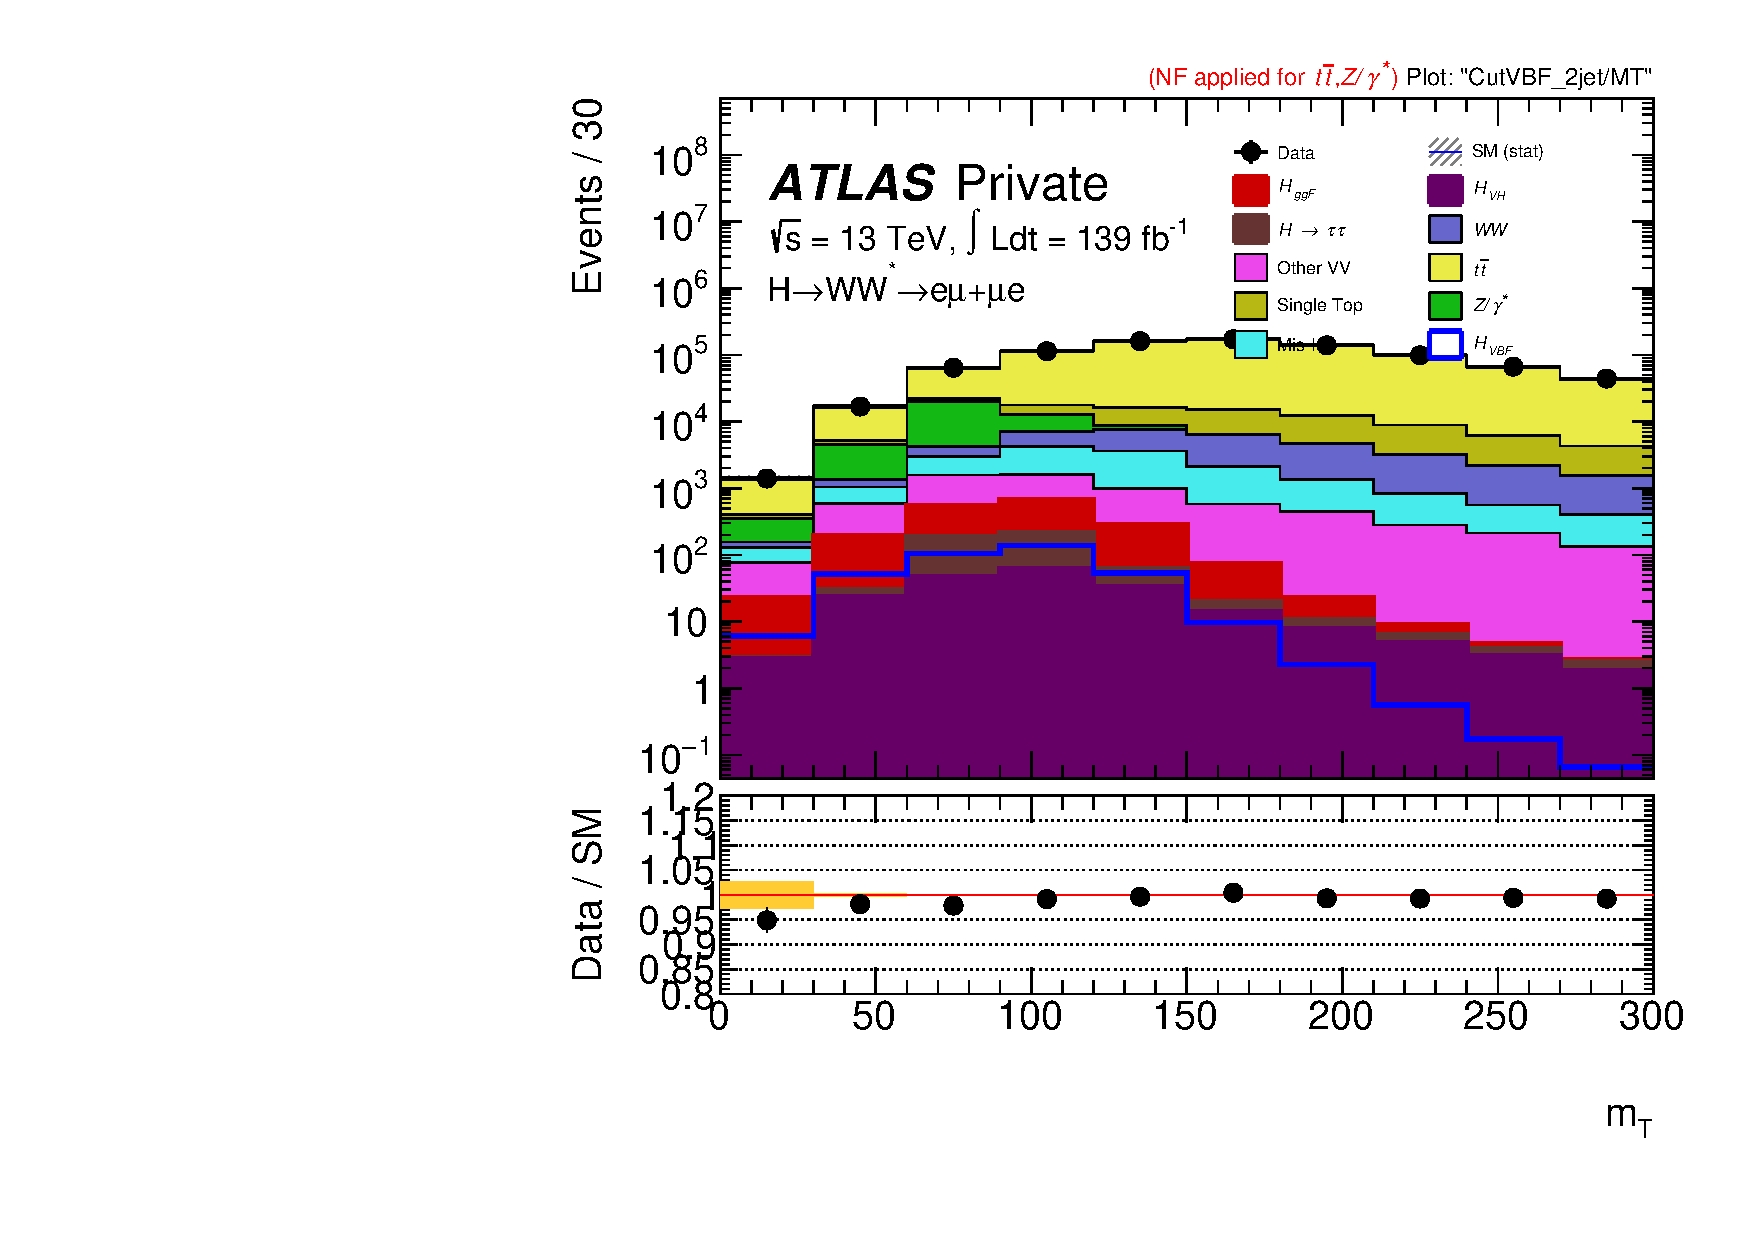
\includegraphics[width=0.3\textwidth]{Pictures/run2-emme-CutVBF_2jet-MT-log.pdf}
  }\hfill
%  \subfloat[$p^T_{tot}$]{
%      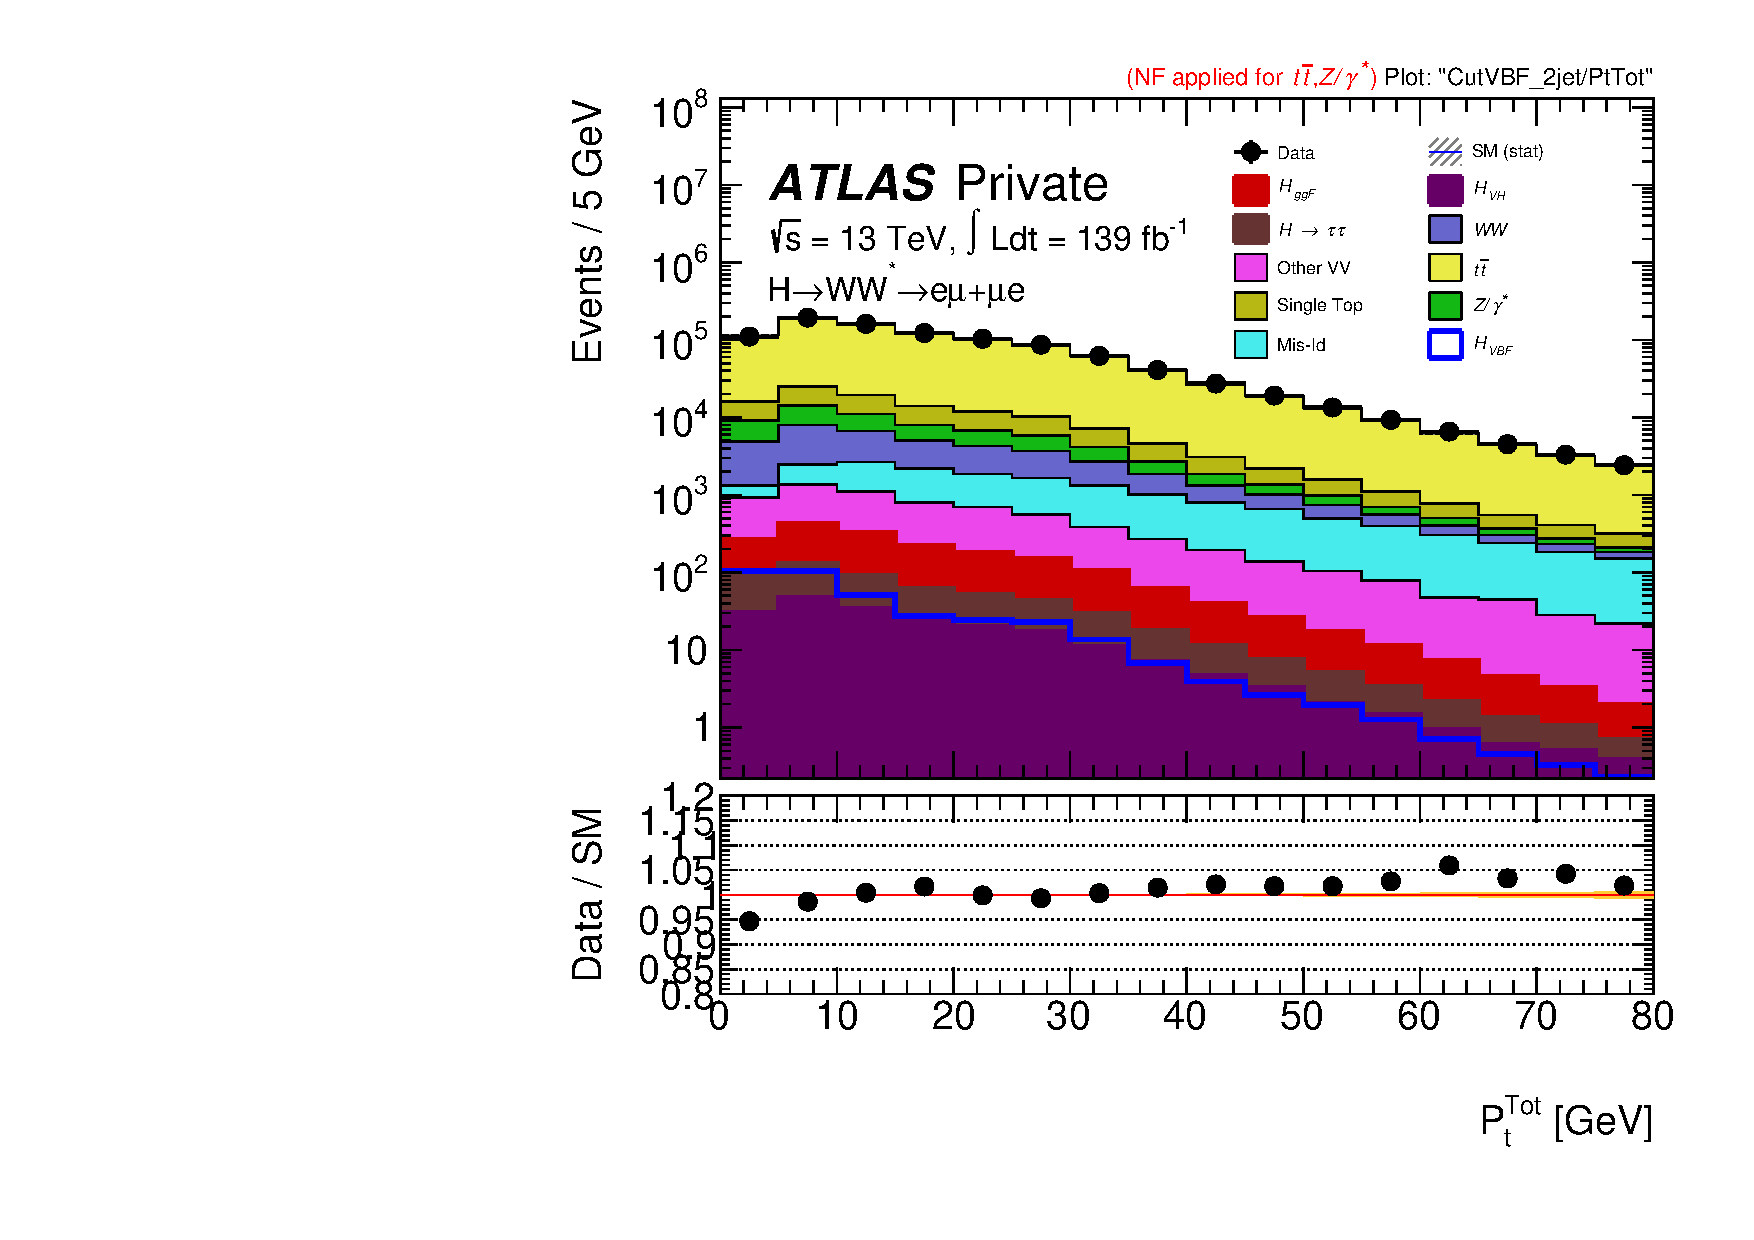
\includegraphics[width=0.3\textwidth]{Pictures/run2-emme-CutVBF_2jet-PtTot-log.pdf}
%  }\hfill
%  \subfloat[lep $p^T_{\text{lead}}$]{
%      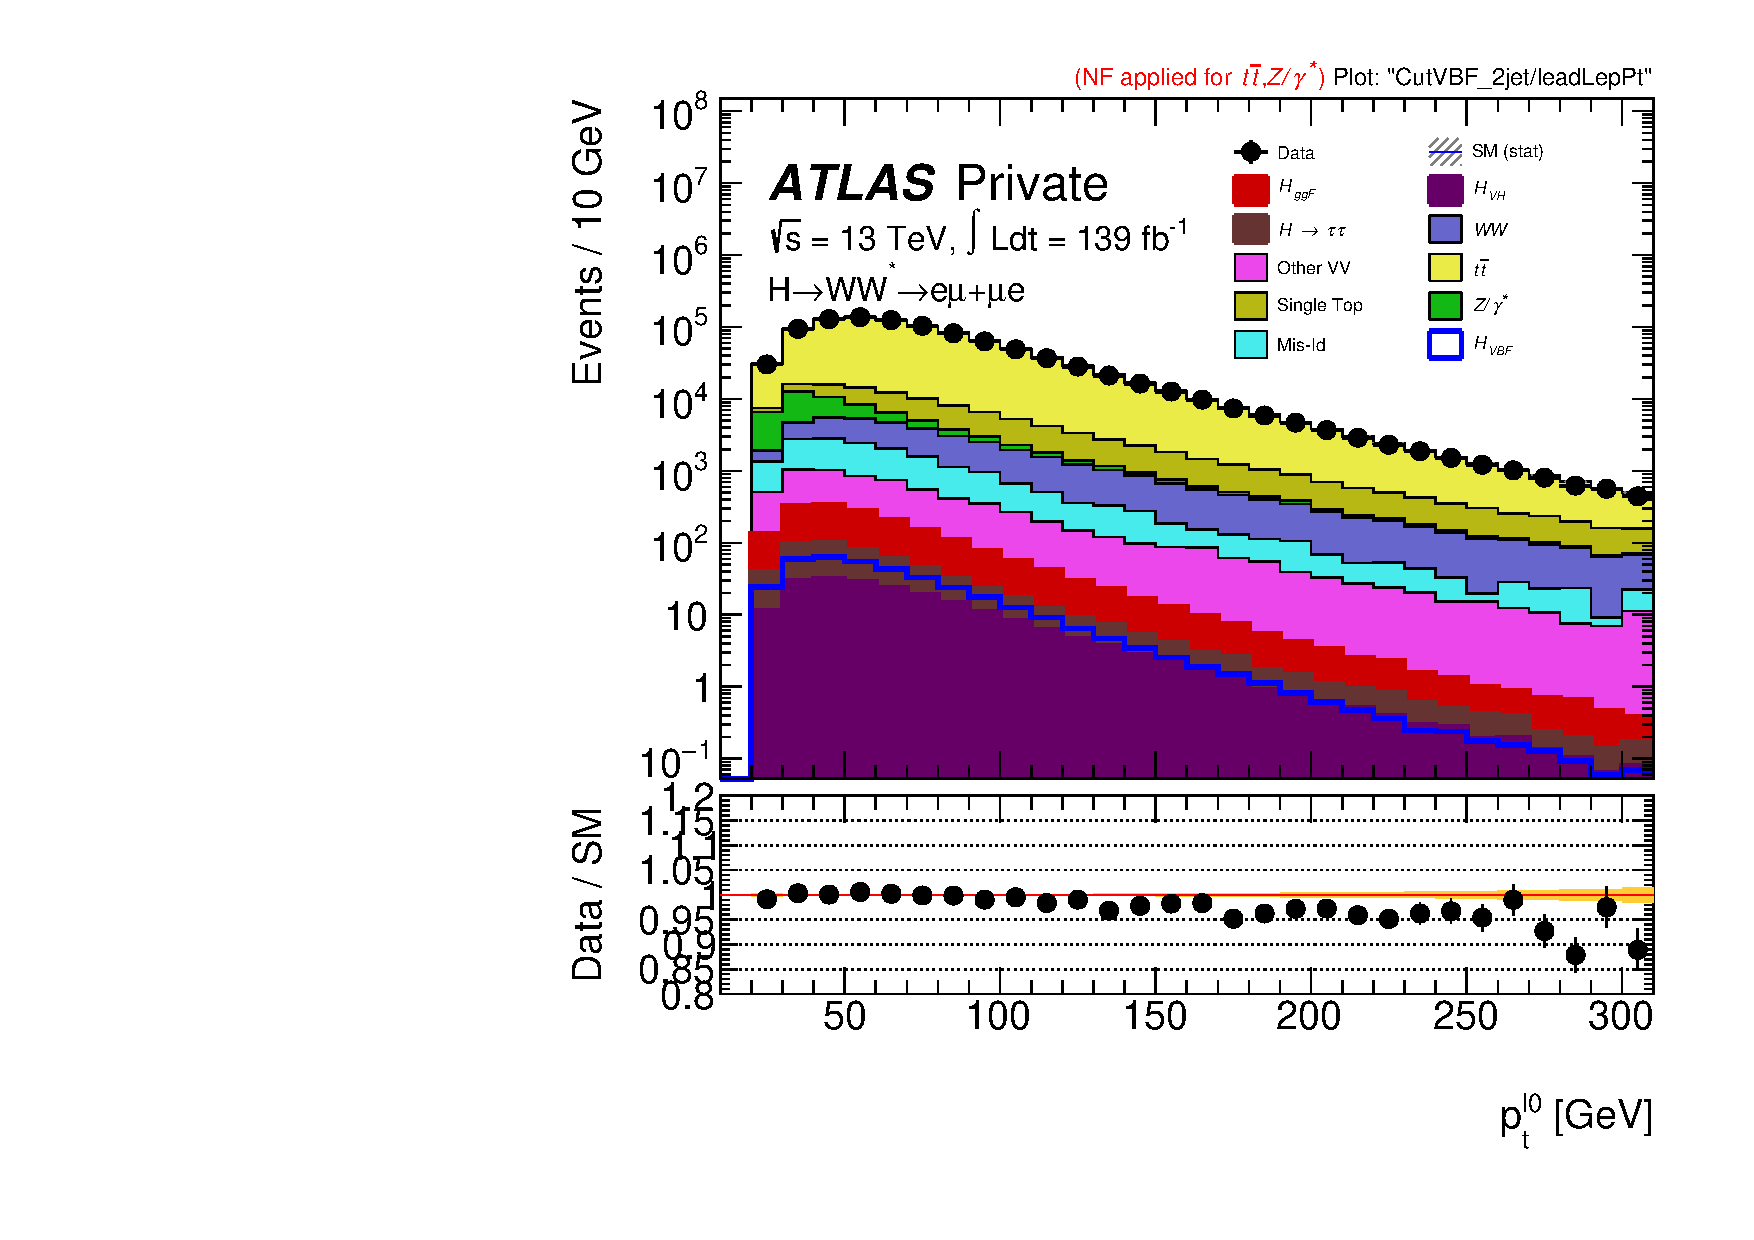
\includegraphics[width=0.3\textwidth]{Pictures/run2-emme-CutVBF_2jet-leadLepPt-log.pdf}
%  }\hfill
  \subfloat[jet $p^T_{\text{lead}}$]{
      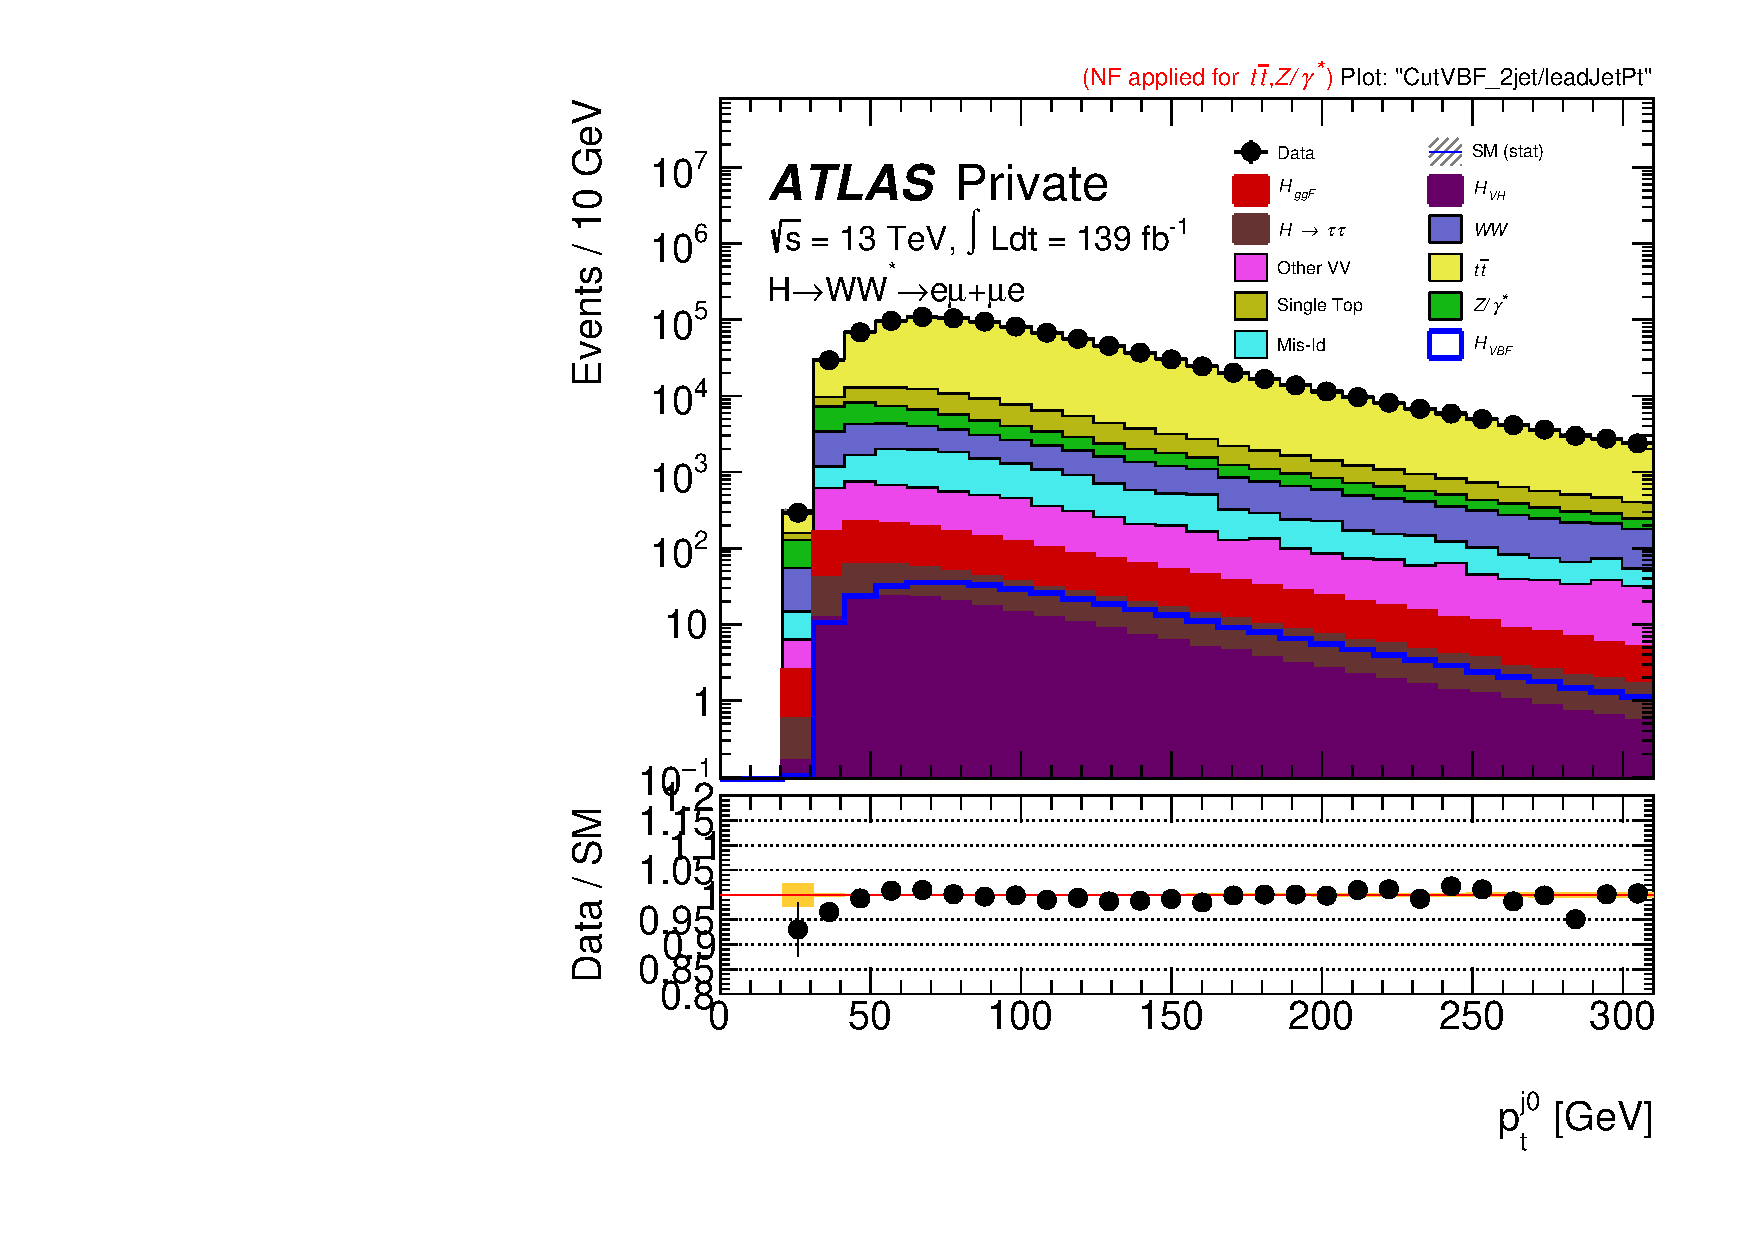
\includegraphics[width=0.3\textwidth]{Pictures/run2-emme-CutVBF_2jet-leadJetPt-log.pdf}
  }\hfill
%  \subfloat[lep $p^T_{\text{sublead}}$]{
%      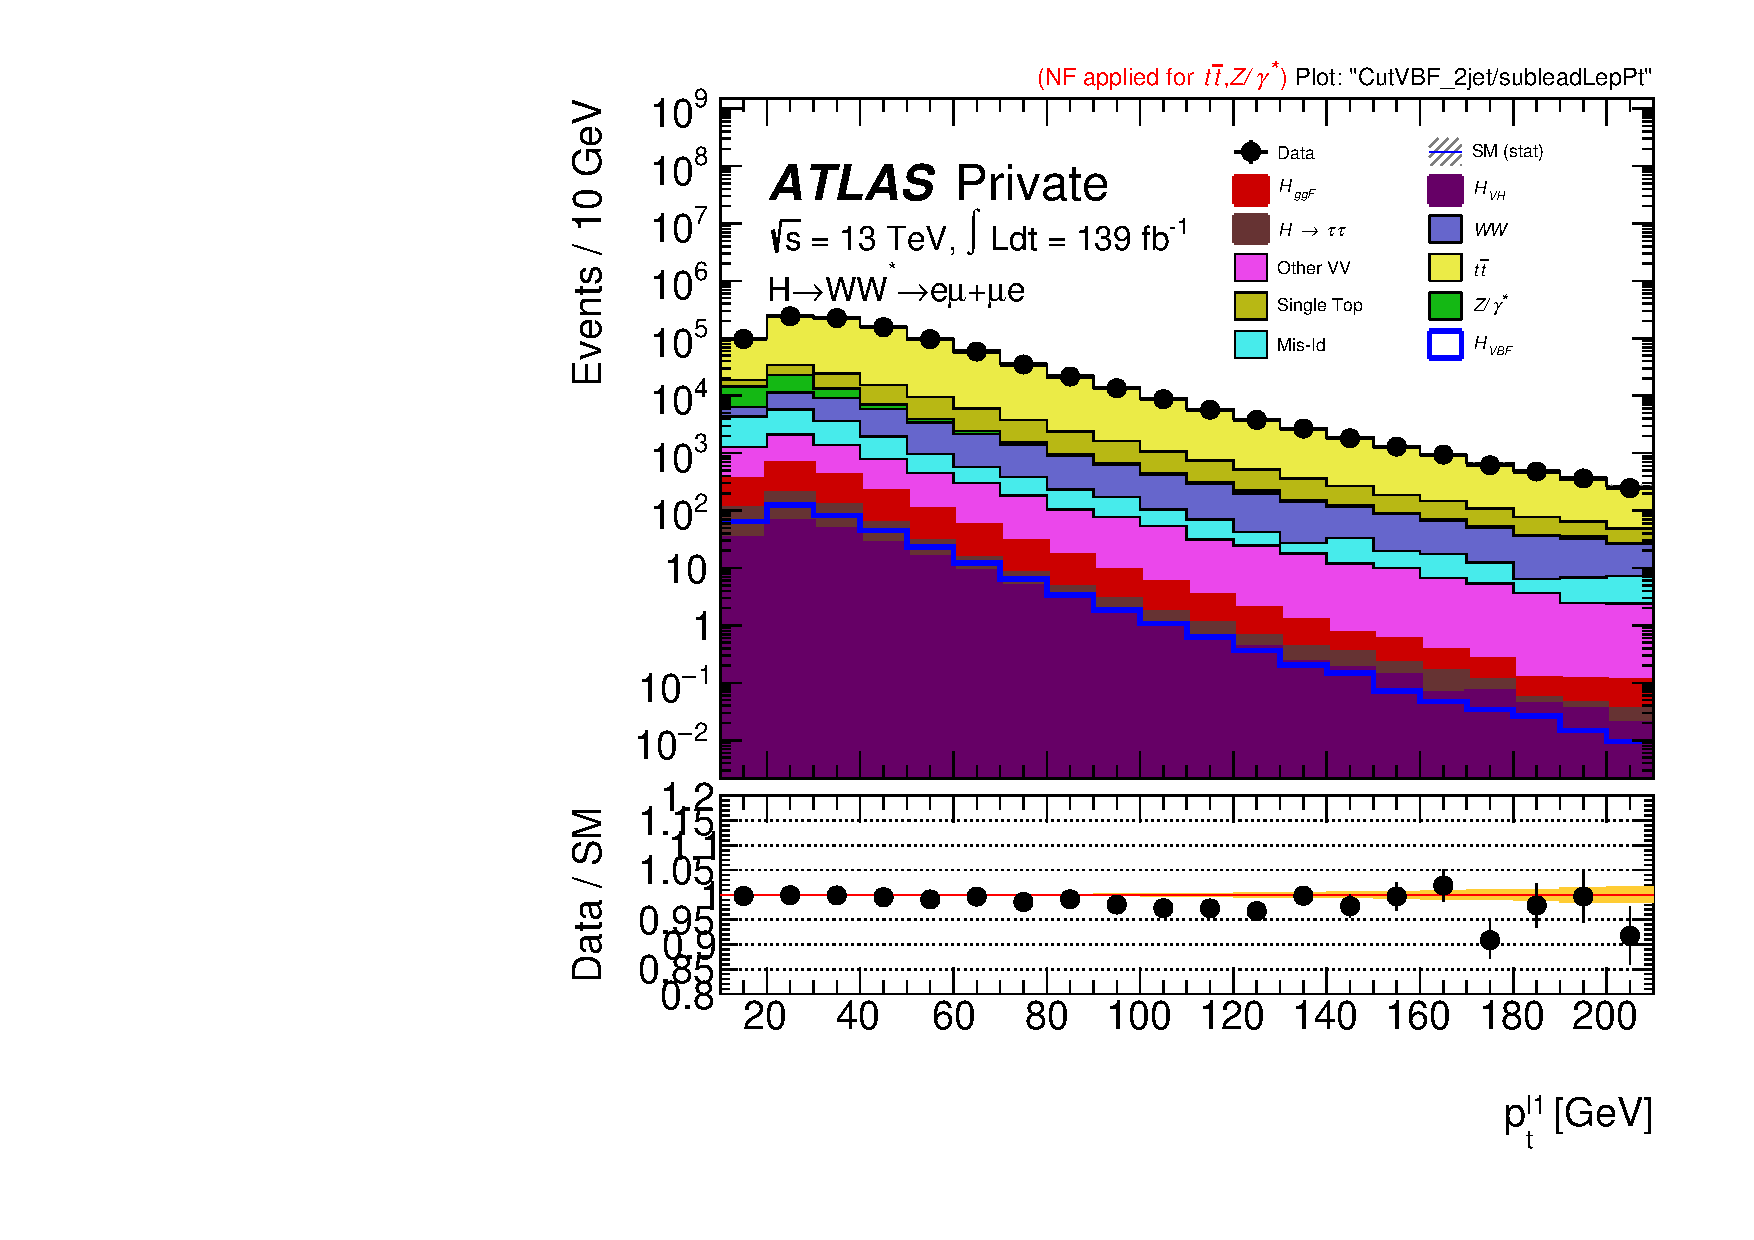
\includegraphics[width=0.3\textwidth]{Pictures/run2-emme-CutVBF_2jet-subleadLepPt-log.pdf}
%  }\hfill
  \subfloat[jet $p^T_{\text{sublead}}$]{
      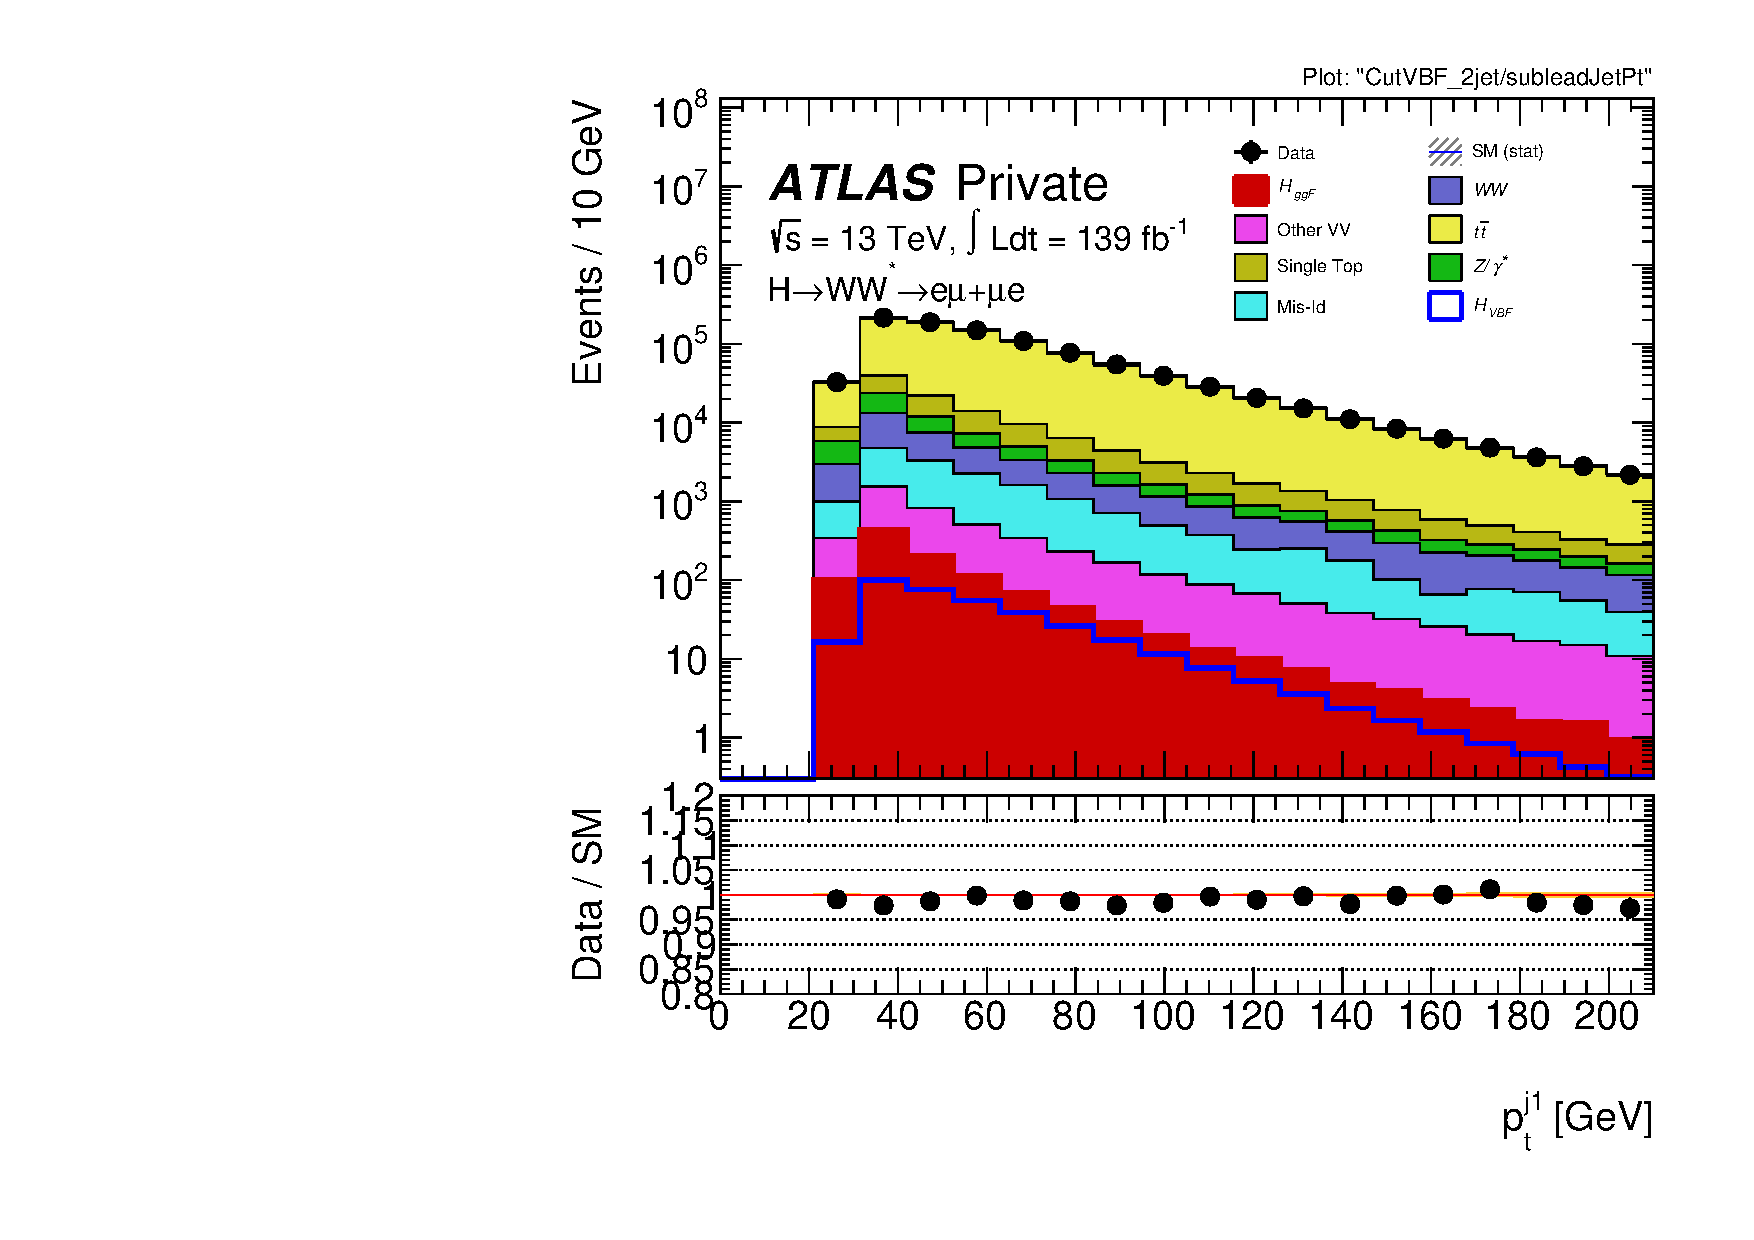
\includegraphics[width=0.3\textwidth]{Pictures/run2-emme-CutVBF_2jet-subleadJetPt-log.pdf}
  }\hfill
  \subfloat[$\Delta \phi_{jj}$]{
      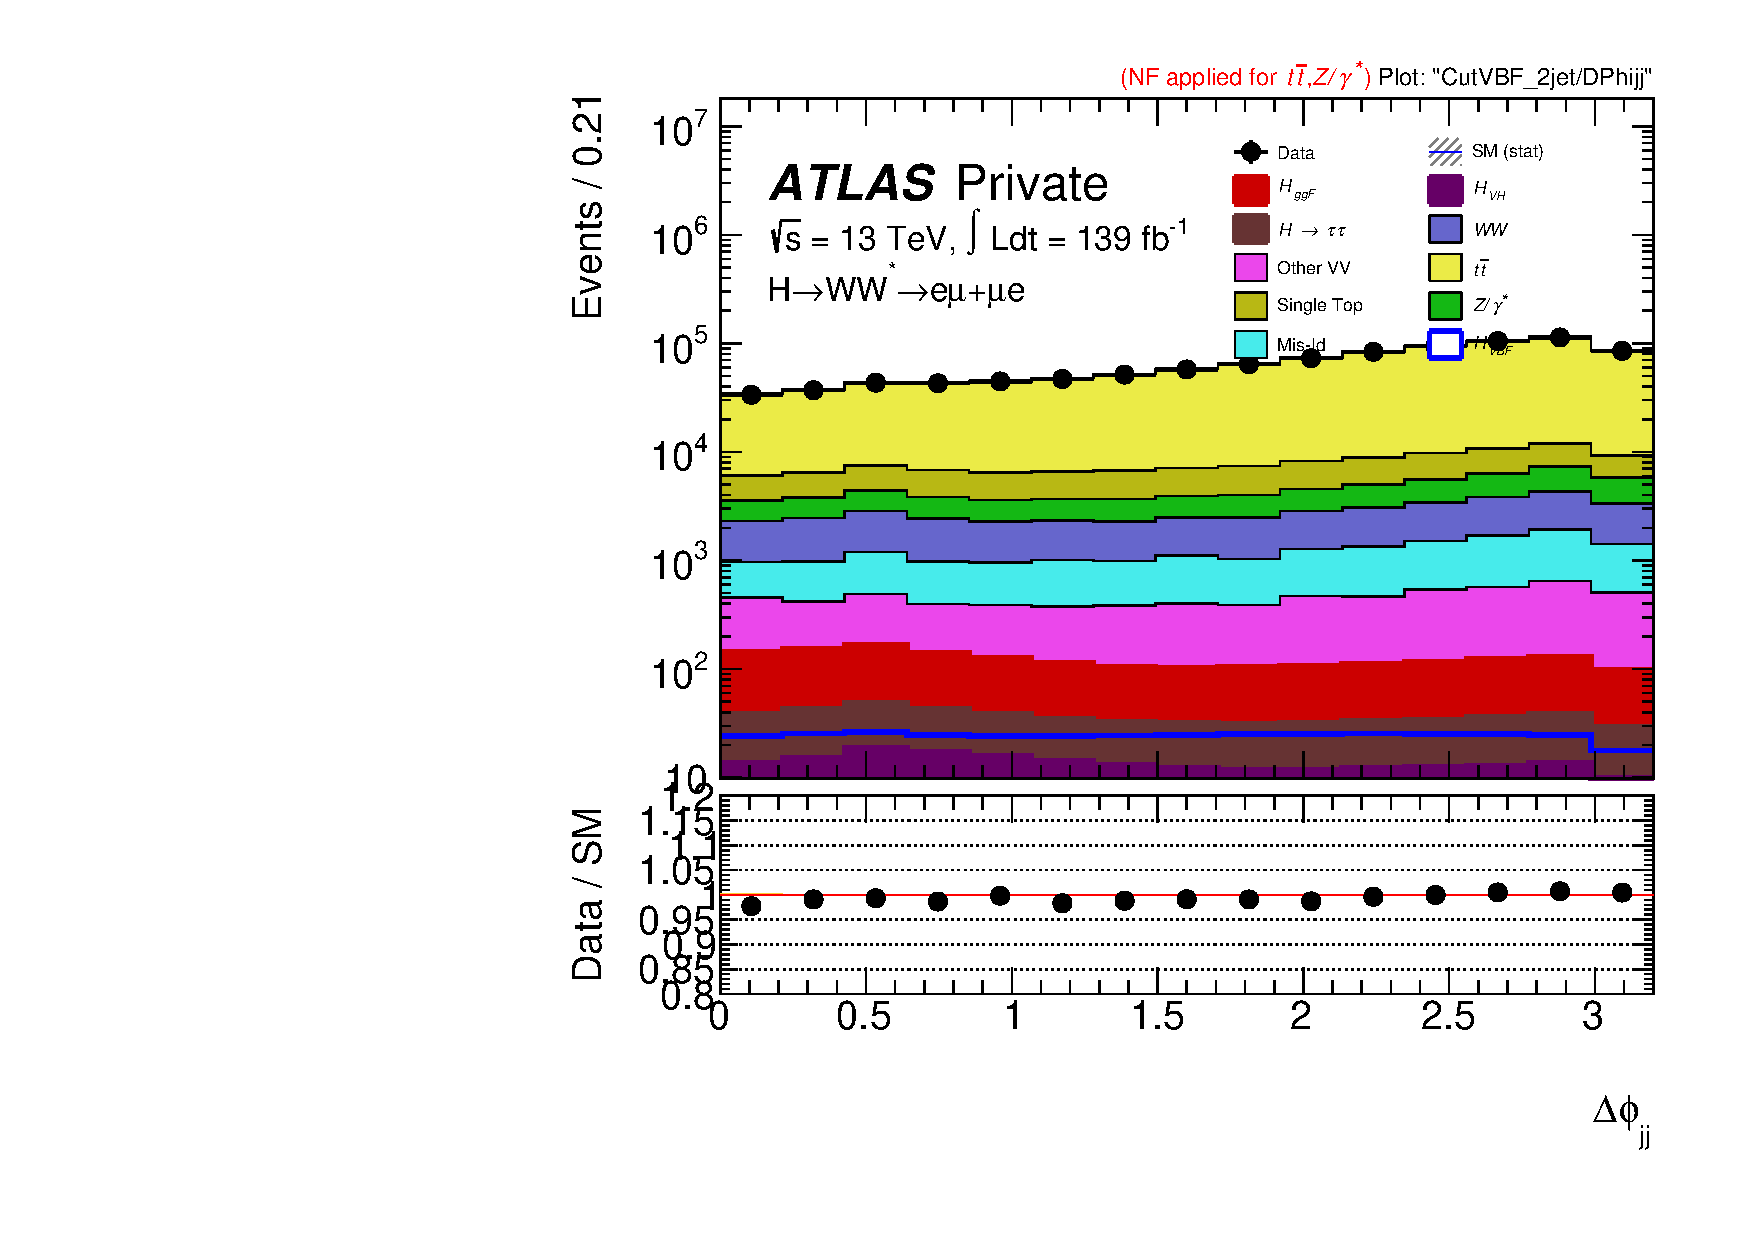
\includegraphics[width=0.3\textwidth]{Pictures/run2-emme-CutVBF_2jet-DPhijj-log.pdf}
  }%\hfill
%  \subfloat[$\ensuremath{E_{\text{T,rel}}^{\text{miss}}}$]{
%      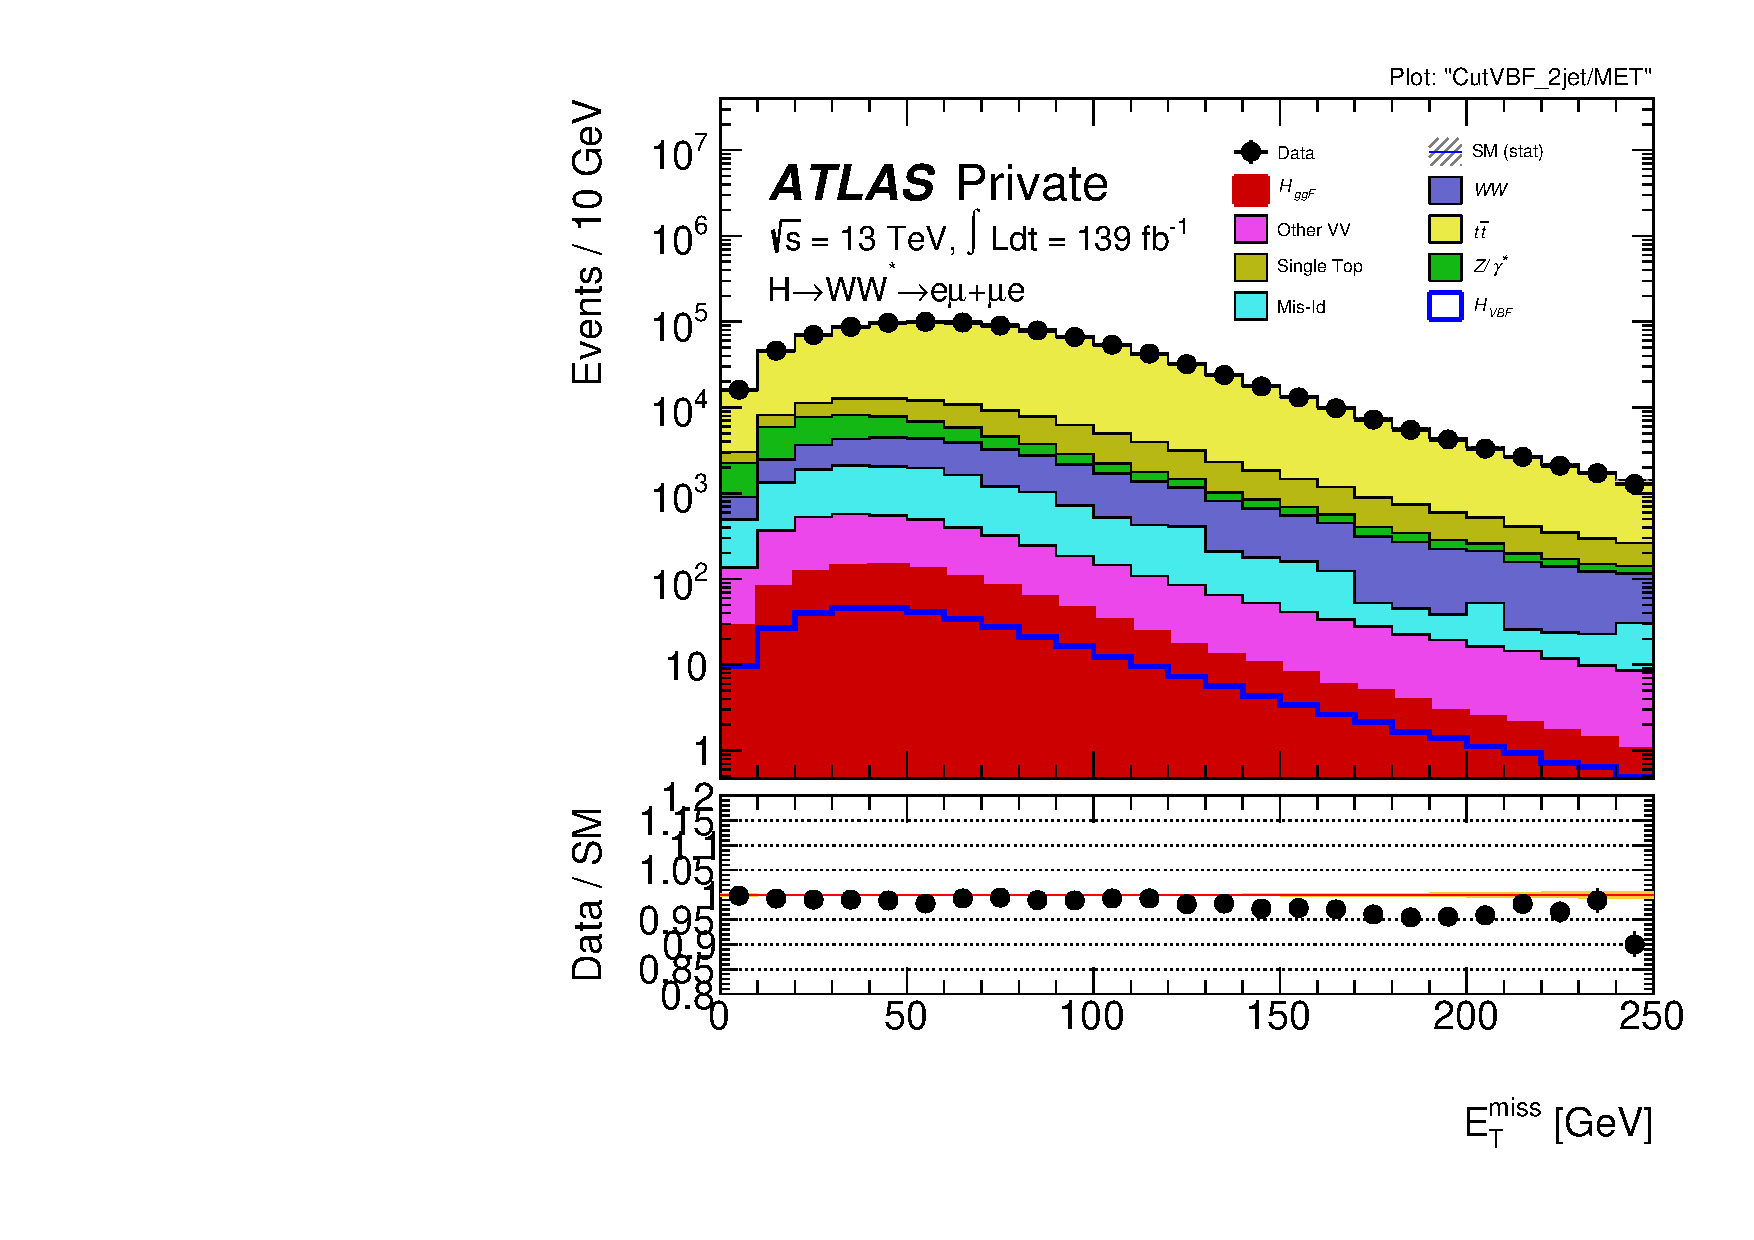
\includegraphics[width=0.3\textwidth]{Pictures/run2-emme-CutVBF_2jet-MET-log.pdf}
%  }%\hfill
{\caption{Distributions of $\Delta Y_{jj}$, $\Delta Y_{\ell\ell}$, $\Delta \phi_{\ell\ell}$, $m_{jj}$, $m_{\ell\ell}$,$m_T$, jet $p^T_{\text{lead}}$, jet $p^T_{\text{sublead}}$, and $\Delta \phi_{jj}$ in the preselection region. Distributions show good MC modeling of variables used in the signal region BDT.
\label{fig:preselection}}}
\end{figure} 

\subsection{Signal region selection}
In addition to the pre-selection cuts which are in common with the ggF coupling analysis, additional selection criteria are applied to the VBF signal region. These selections include a requirement for at least 2 jets ($n_{jets}>=2$) and a $b$-veto using the DL1r $b$-tagging algorithm. A central-jet-veto (CJV) and an outside-lepton-veto (OLV) are also applied. These remove first events with $p_T >20$ GeV which lie between the tagging jets in pseudo-rapidity and next any event where the two charged leptons are not within the tagging jets' rapidity gap. Two additional cuts that differ form the VBF HWW couplings analysis are also added. These require that the mass of the two jets be $>200$ GeV and that the rapidity difference between the two jets be $>2.1$. These further purify the signal region against a range of backgrounds, notably top. The plots in Figure~\ref{fig:MjjDYjjSig} show signal and background yields as well as signal significance at a variety of $m_{jj}$ and $\Delta Y_{jj}$ values. The values used here are chosen for their effects on signal significance while retaining high signal statistics. 

\begin{figure}[!htbp]
\centering
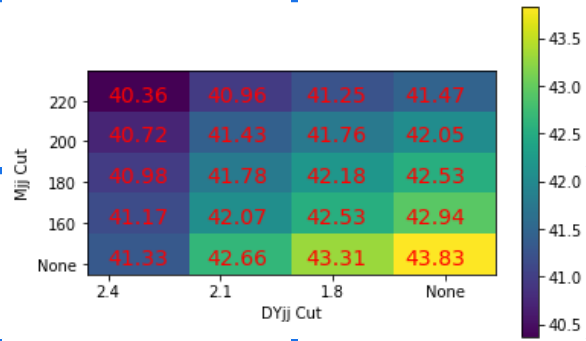
\includegraphics[width=.3\linewidth]{Pictures/MjjDYjjVBF.png}
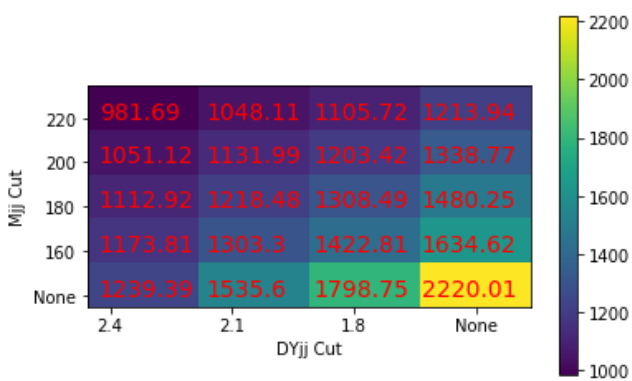
\includegraphics[width=.3\linewidth]{Pictures/MjjDYjjBackground.png}
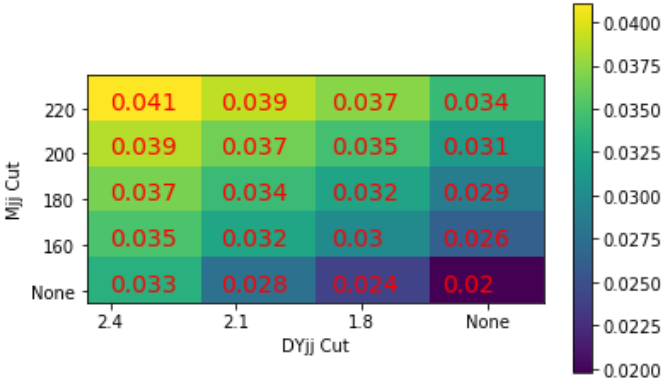
\includegraphics[width=.3\linewidth]{Pictures/MjjDYjjSig.png}
\caption{Signal and be background yields for VBF and total background (aside from fakes) at various $m_{jj}$ and $\Delta Y_{jj}$ cut values. Simulated events for MC16a campaign only. Choice of cut at $m_{jj}>200$GeV and $DY_{jj}>2.1$ nearly halves background yields while reducing signal by $<5\%$.}
\label{fig:MjjDYjjSig}
\end{figure}

Signal region cuts are listed in Table~\ref{tab:SRdef}.  

\begin{table}[h!]
\centering
\resizebox{\textwidth}{!}{
\begin{tabular}{|l|c|c|c|}
\hline
\multirow{2}{*}{Signal region cut}   & Description \\
					&	\\
\hline
2-jet (30,30)           & Require at least 2 jets with $p_T \geq 30$GeV\\
$b$-veto      		& Use DL1 efficiency $b$-tag reject events with $b$-jets/apply $b$-tag weight \\
Blinding (VBF)          & Blinding condition on data (cut on VBF vs. Top$+WW$ BDT) \\
CJV ($20$GeV)		& Cut events with a third central rapidity jet $p_T > 20$GeV \\
OLV bool	        & Leading lepton $\eta$ required to be between two $\eta$ 2 leading jets \\
$Z\rightarrow\tau\tau$ veto & $m_{\tau\tau} < m_Z - 25$GeV \\ 
$m_{jj}$ cut		& $m_{jj} > 200$GeV \\
$\Delta Y_{jj}$ cut	& $\Delta Y_{jj} > 2.1$ \\
\hline
\end{tabular}}
\caption{Table describing VBF signal region cuts}
\label{tab:SRdef}
\end{table}

Yields for all samples, as well as data for signal region cuts are shown in Table~\ref{tab:srcut}.
\begin{table}[h!]
\resizebox{\textwidth}{!}{
%%% created on Thu May 28 12:37:09 2020 from TQSampleFolder 'samples' with TQLibrary UNKNOWN compiled with GCC 8.3.0 against ROOT 6.16/00
\providecommand{\xmark}{{\sffamily \bfseries X}}
\providecommand\rotatecell[2]{\rotatebox[origin=c]{#1}{#2}}
\begin{tabular}{ r || r  r  r  | r  r || r  r  | r  r  r  r }
\ensuremath{\mathcal{L}=139 fb^{-1}} & $H_{VBF}$ & $H_{ggF}$  & $H \rightarrow \tau\tau$ & $WW$ & Top & Zjets & Mis-Id & Total Bkg & Significance & Data & Data/MC\tabularnewline
\hline
2-jet (30,30) fJVT & \ensuremath{366.47\pm 0.58} & \ensuremath{1295.72\pm 3.71} & \ensuremath{341.06\pm 1.18} & \ensuremath{24353.25\pm 30.46} & \ensuremath{911102.17\pm 201.73} & \ensuremath{26401.33\pm 108.44} & \ensuremath{11519.17\pm 164.08} & \ensuremath{980281.52\pm 300.00} & \ensuremath{0.37\pm 0.00} & \ensuremath{976091} & \ensuremath{1.00\pm 0.00}\tabularnewline
b-veto & \ensuremath{323.67\pm 0.54} & \ensuremath{1109.94\pm 3.42} & \ensuremath{287.53\pm 1.07} & \ensuremath{21075.69\pm 28.85} & \ensuremath{63787.91\pm 57.22} & \ensuremath{22151.24\pm 102.73} & \ensuremath{3793.55\pm 70.69} & \ensuremath{116387.21\pm 168.10} & \ensuremath{0.95\pm 0.00} & \ensuremath{109677} & \ensuremath{0.94\pm 0.00}\tabularnewline
blinding (2-jet) & \ensuremath{323.67\pm 0.54} & \ensuremath{1109.94\pm 3.42} & \ensuremath{287.53\pm 1.07} & \ensuremath{21075.69\pm 28.85} & \ensuremath{63787.91\pm 57.22} & \ensuremath{22151.24\pm 102.73} & \ensuremath{3793.55\pm 70.69} & \ensuremath{116387.21\pm 168.10} & \ensuremath{0.95\pm 0.00} & \ensuremath{107456} & \ensuremath{0.92\pm 0.00}\tabularnewline
CJV (20GeV) & \ensuremath{256.58\pm 0.48} & \ensuremath{807.85\pm 2.92}  & \ensuremath{214.70\pm 0.92} & \ensuremath{15050.73\pm 24.95} & \ensuremath{43135.02\pm 47.62} & \ensuremath{16159.77\pm 89.34} & \ensuremath{2629.36\pm 59.14} & \ensuremath{81067.63\pm 144.34} & \ensuremath{0.90\pm 0.00} & \ensuremath{75589} & \ensuremath{0.93\pm 0.00}\tabularnewline
OLV bool & \ensuremath{199.59\pm 0.43} & \ensuremath{218.02\pm 1.52}  & \ensuremath{75.81\pm 0.47} & \ensuremath{2741.46\pm 11.72} & \ensuremath{9418.19\pm 22.26} & \ensuremath{3664.17\pm 45.30} & \ensuremath{460.46\pm 26.24} & \ensuremath{17212.14\pm 68.78} & \ensuremath{1.52\pm 0.00} & \ensuremath{15644} & \ensuremath{0.90\pm 0.01}\tabularnewline
$Z\to\tau\tau$ veto & \ensuremath{172.20\pm 0.40} & \ensuremath{192.86\pm 1.43}  & \ensuremath{12.62\pm 0.22} & \ensuremath{1701.95\pm 9.30} & \ensuremath{6057.49\pm 17.83} & \ensuremath{1331.98\pm 35.93} & \ensuremath{311.20\pm 20.27} & \ensuremath{9979.97\pm 54.56} & \ensuremath{1.72\pm 0.01} & \ensuremath{8971} & \ensuremath{0.88\pm 0.01}\tabularnewline
Mjj$>$200 & \ensuremath{165.51\pm 0.39} & \ensuremath{133.74\pm 1.19}  & \ensuremath{9.99\pm 0.19} & \ensuremath{1160.80\pm 8.03}  & \ensuremath{3568.73\pm 13.73} & \ensuremath{857.97\pm 31.02} & \ensuremath{200.52\pm 15.37} & \ensuremath{6164.63\pm 41.76} & \ensuremath{2.10\pm 0.01} & \ensuremath{5401} & \ensuremath{0.85\pm 0.01}\tabularnewline
DYjj$>$2.1 & \ensuremath{163.07\pm 0.39} & \ensuremath{121.34\pm 1.13} & \ensuremath{9.59\pm 0.18} & \ensuremath{1027.28\pm 7.90} & \ensuremath{3005.76\pm 12.74} & \ensuremath{792.65\pm 30.70} & \ensuremath{180.37\pm 14.10} & \ensuremath{5332.00\pm 40.16} & \ensuremath{2.22\pm 0.01} & \ensuremath{4572} & \ensuremath{0.83\pm 0.01}\tabularnewline

\end{tabular}

}
\caption{Cutflow in the signal region.}
\label{tab:srcut}
\end{table}

The following plots in Figure~\ref{fig:signalregion} show kinematic distributions after the described selection. MC predictions show good modeling of data. Uncertainties shown are purely statistical 
\begin{figure}[!h]
  \subfloat[$\Delta Y_{\ell\ell}$]{
      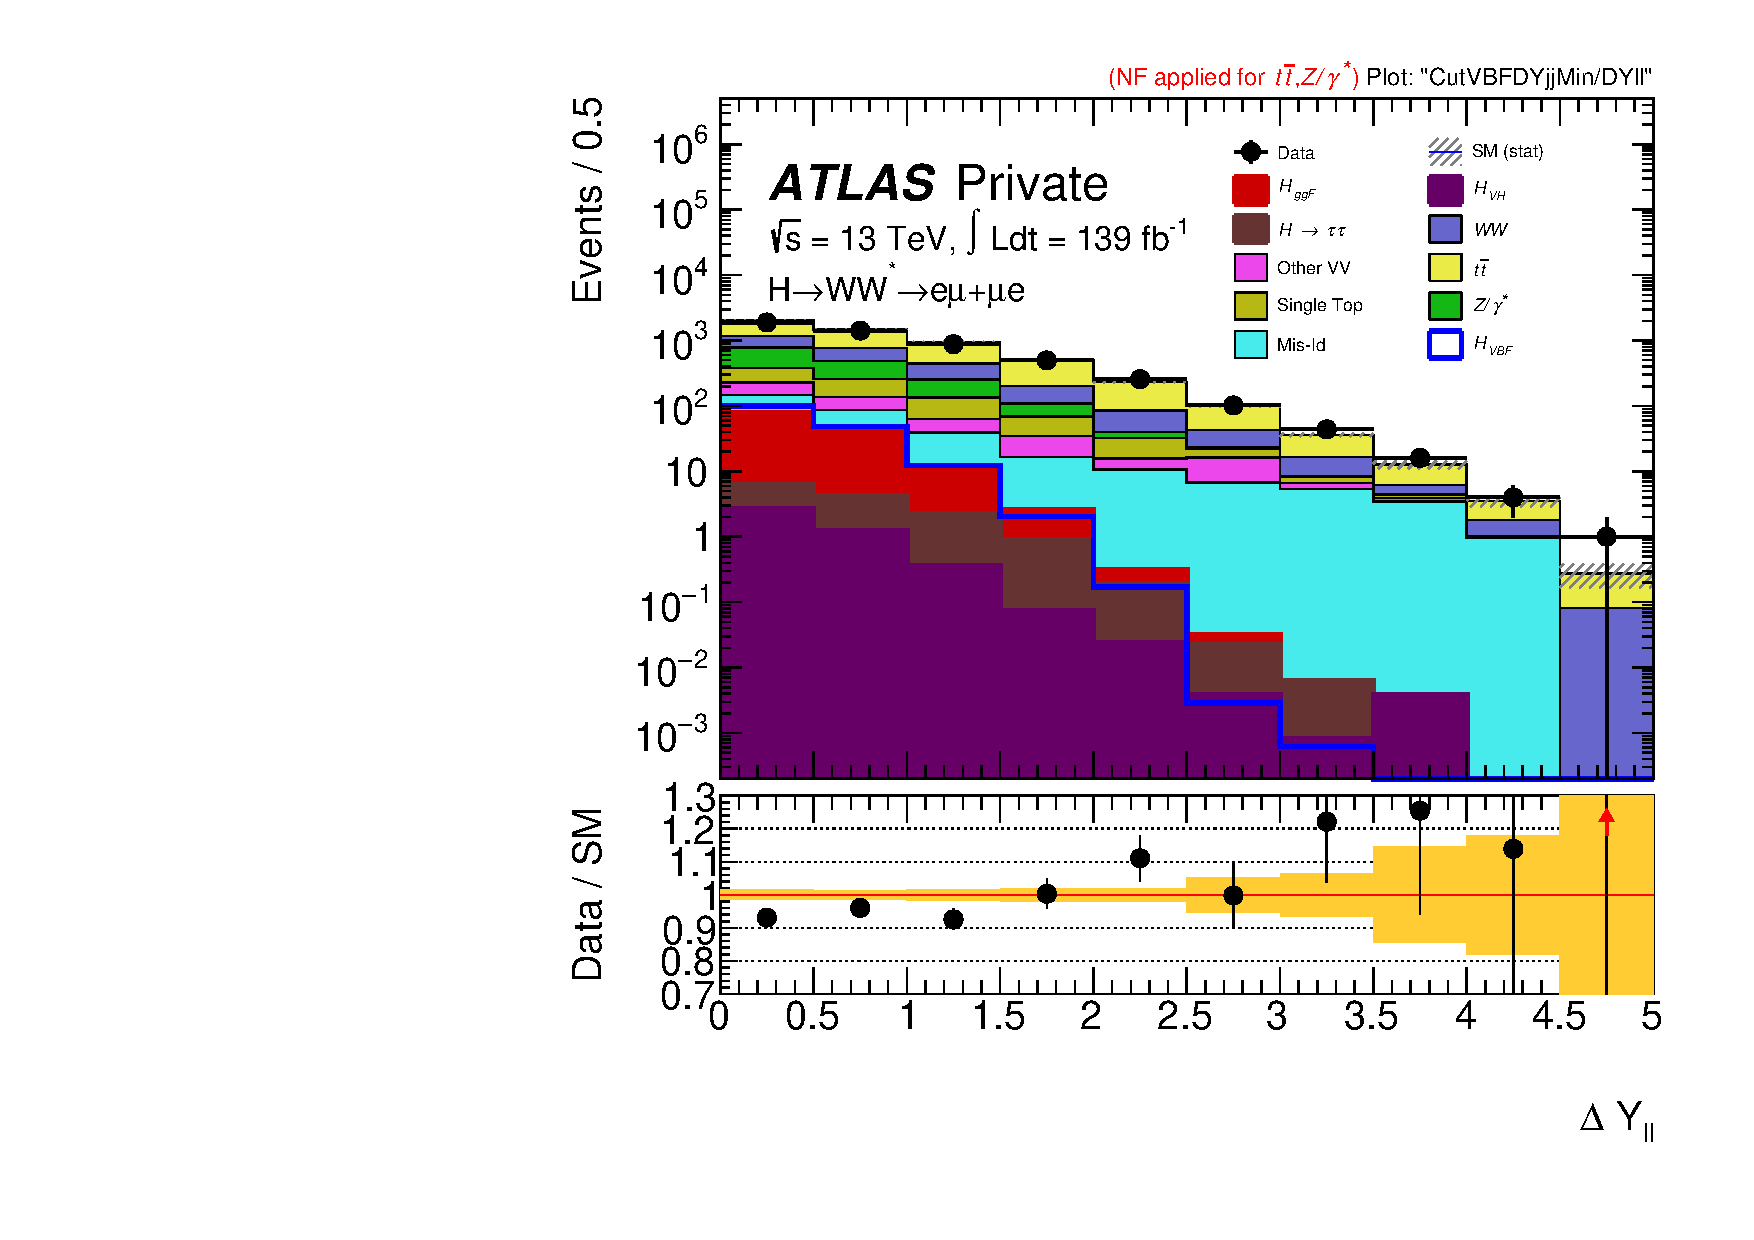
\includegraphics[width=0.3\textwidth]{Pictures/run2-emme-CutVBFDYjjMin-DYll-log.pdf}
  }\hfill
  \subfloat[$\Delta \phi_{\ell\ell}$]{
      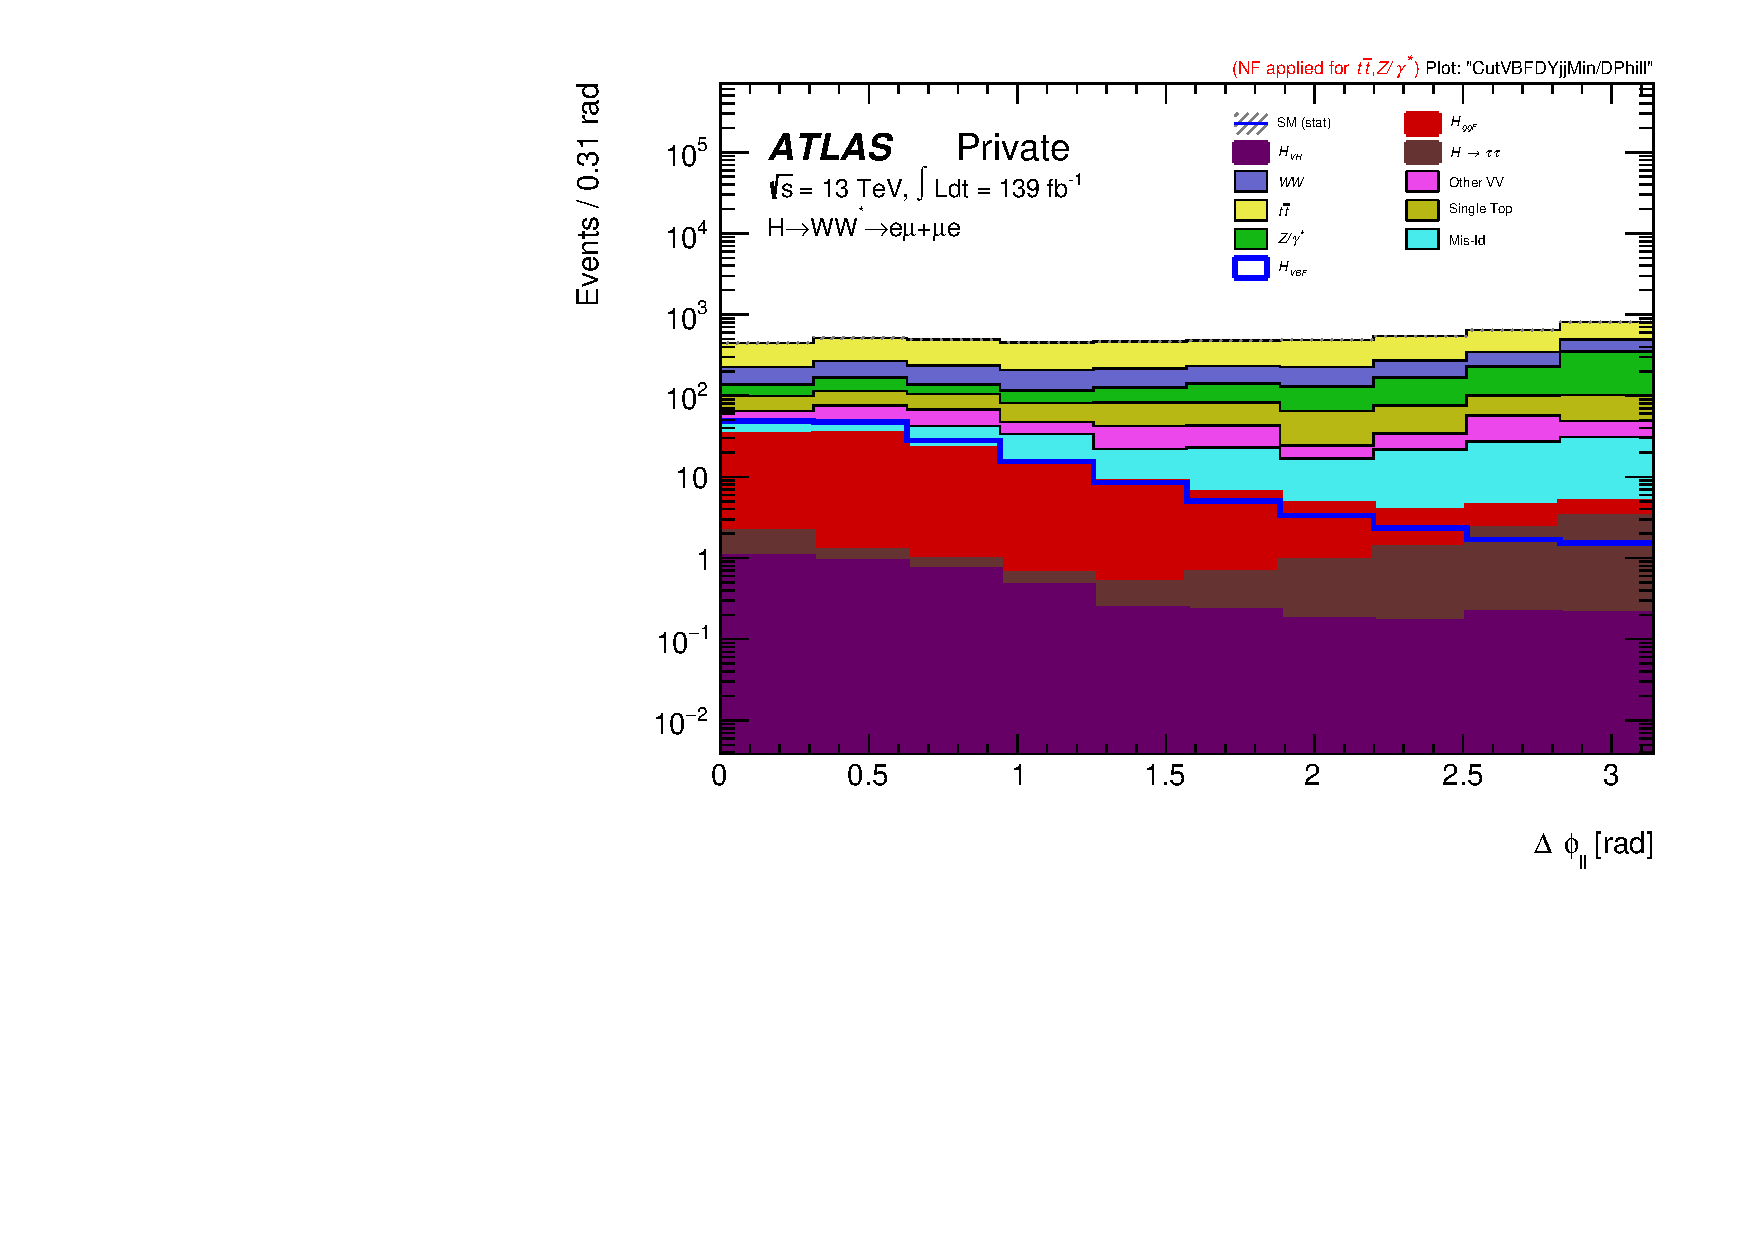
\includegraphics[width=0.3\textwidth]{Pictures/run2-emme-CutVBFDYjjMin-DPhill-log.pdf}
  }\hfill
  \subfloat[$m_{\ell\ell}$]{
      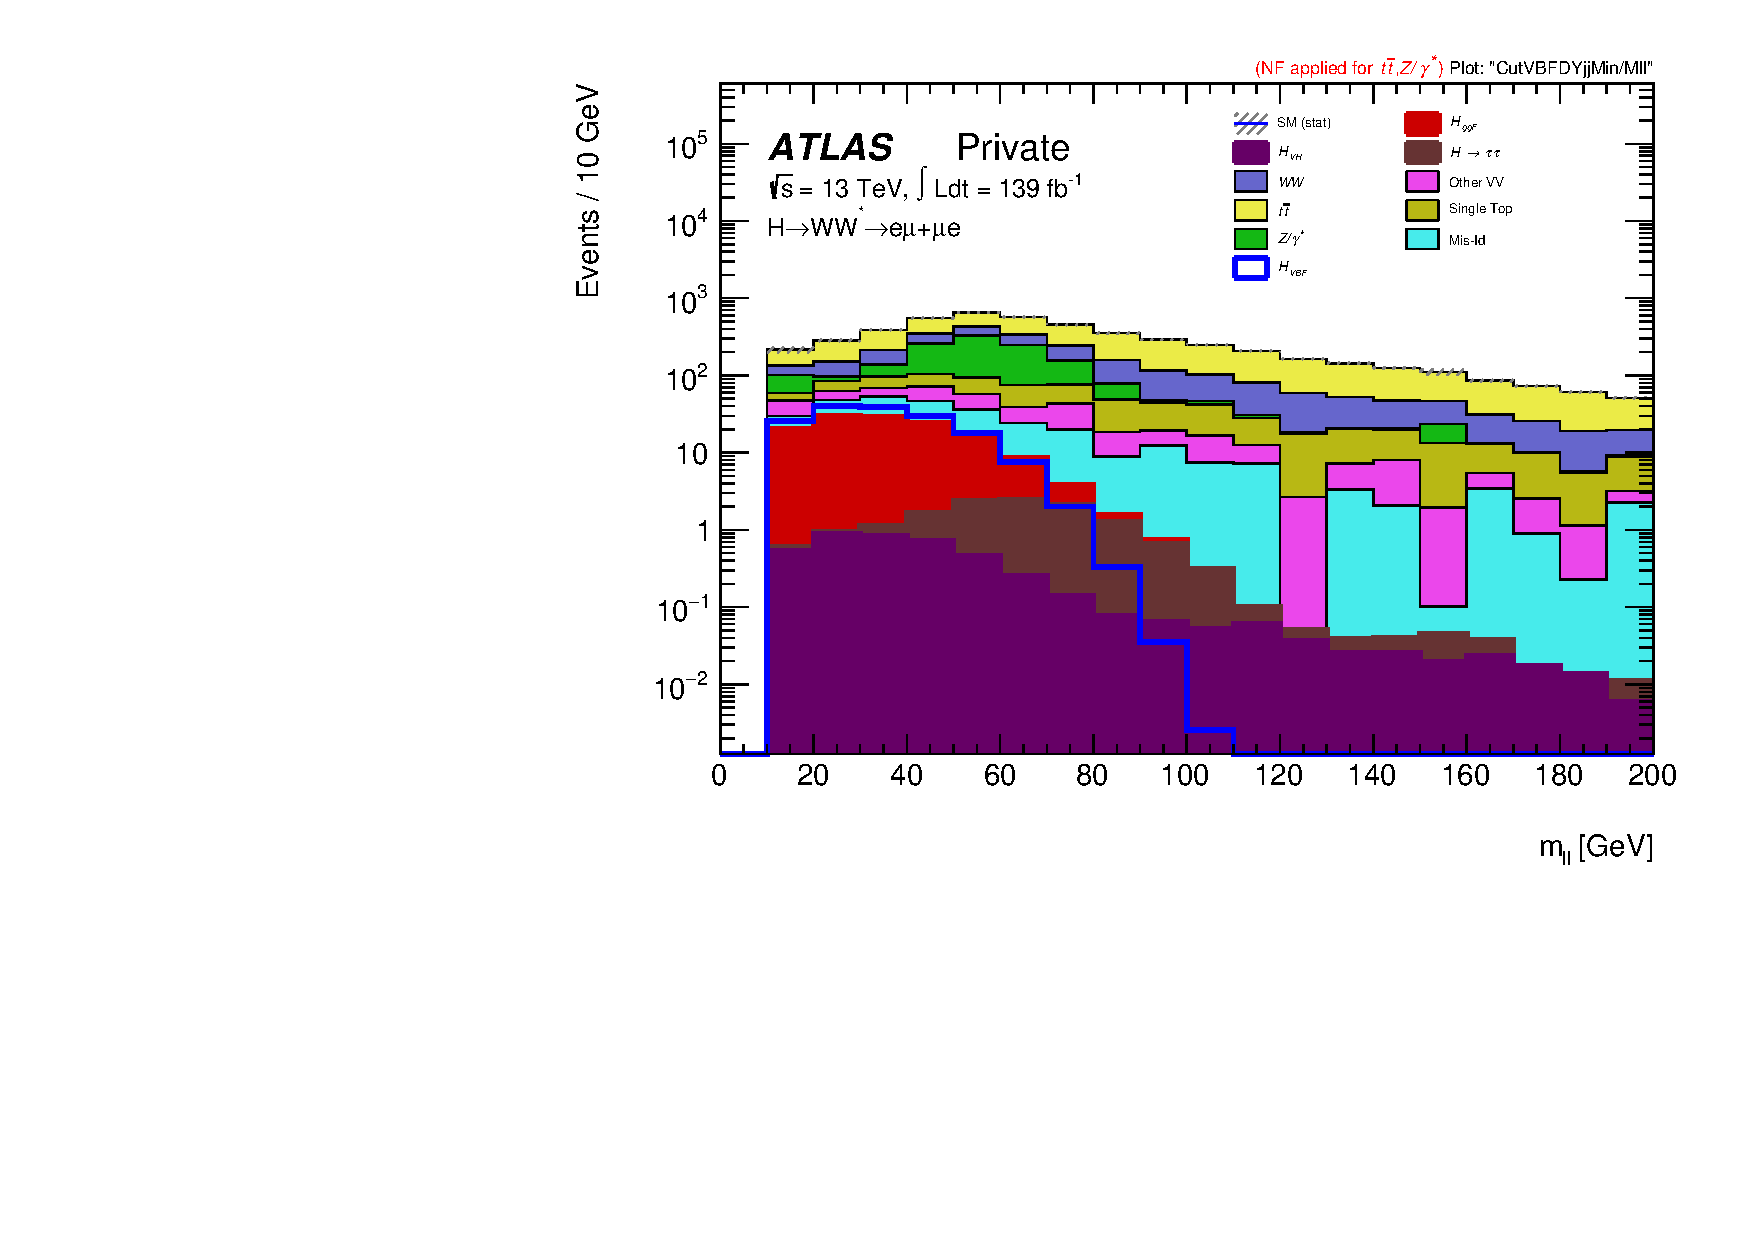
\includegraphics[width=0.3\textwidth]{Pictures/run2-emme-CutVBFDYjjMin-Mll-log.pdf}
  }\hfill
  \subfloat[$m_T$]{
      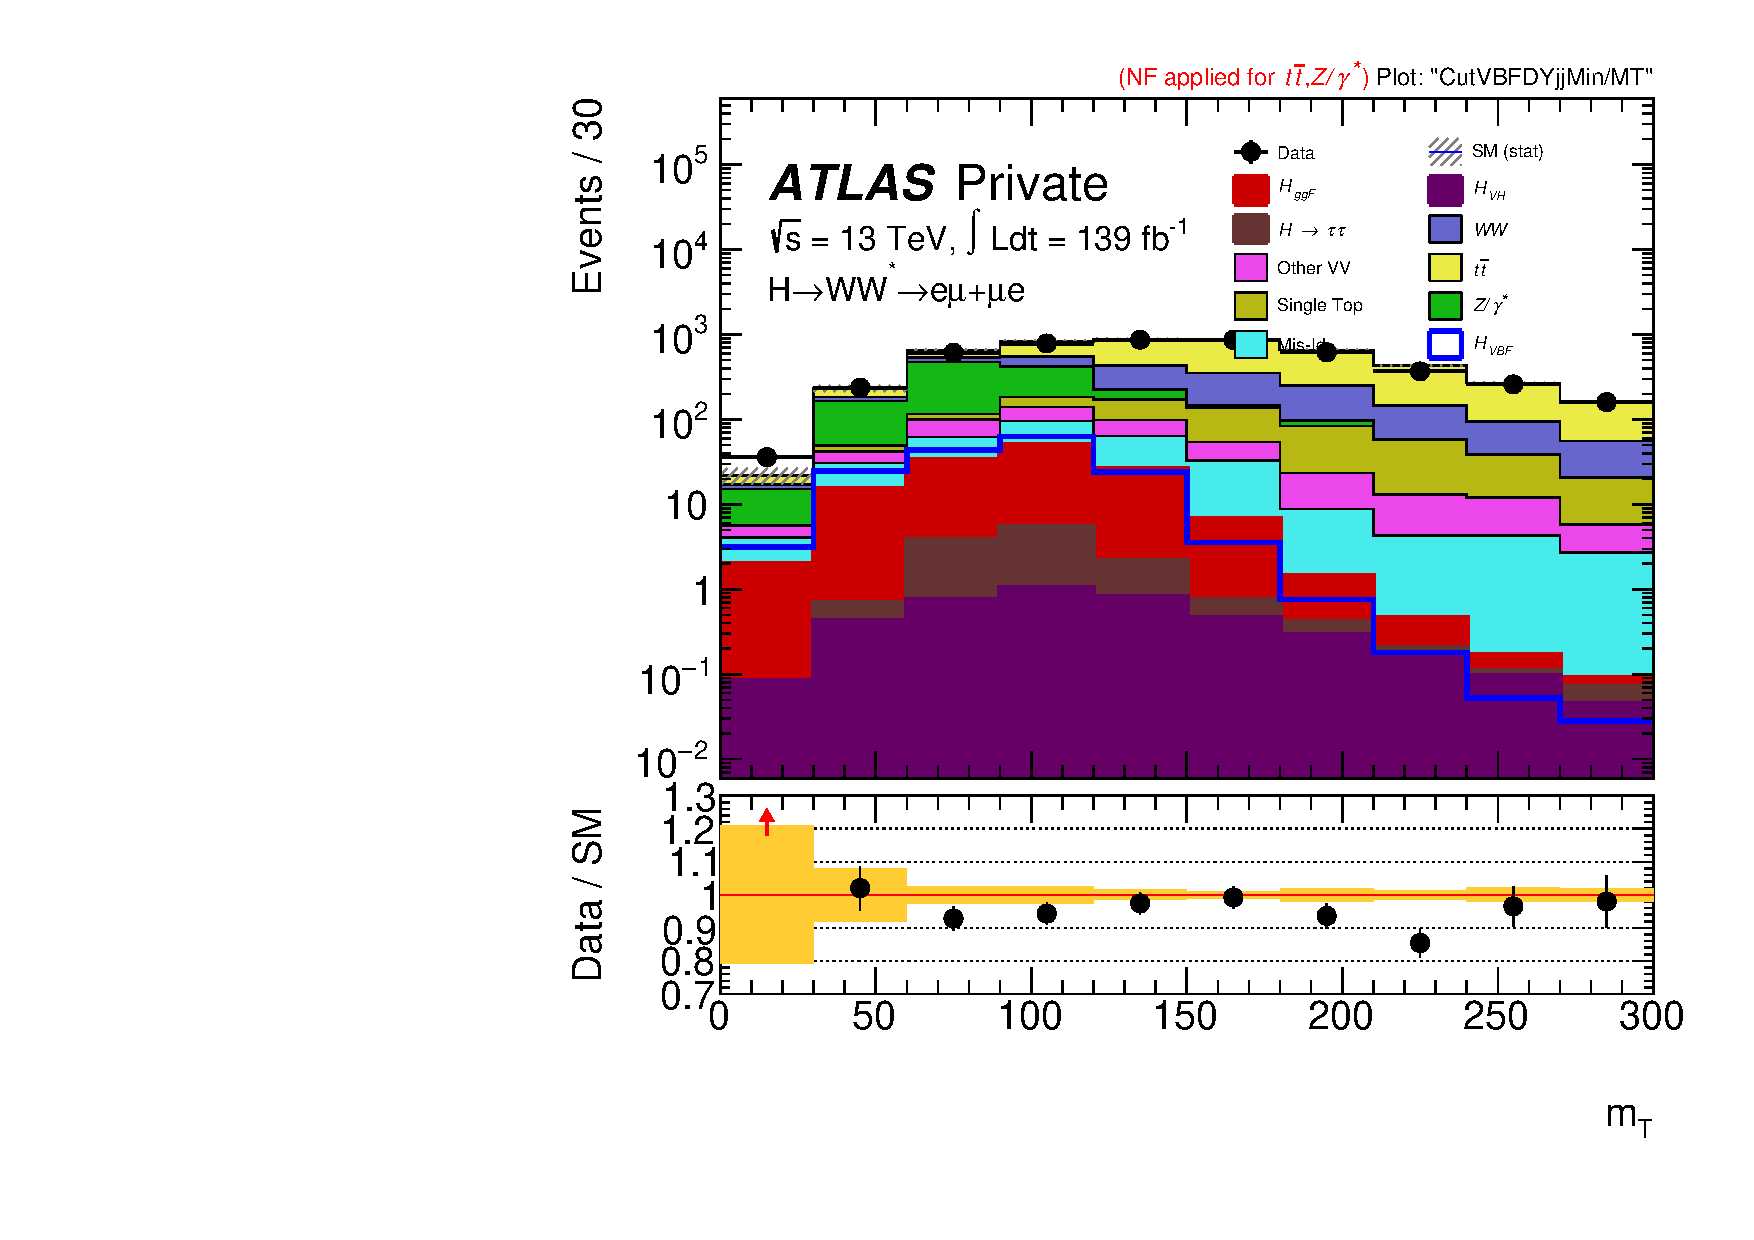
\includegraphics[width=0.3\textwidth]{Pictures/run2-emme-CutVBFDYjjMin-MT-log.pdf}
  }\hfill
  \subfloat[$p^T_{tot}$]{
      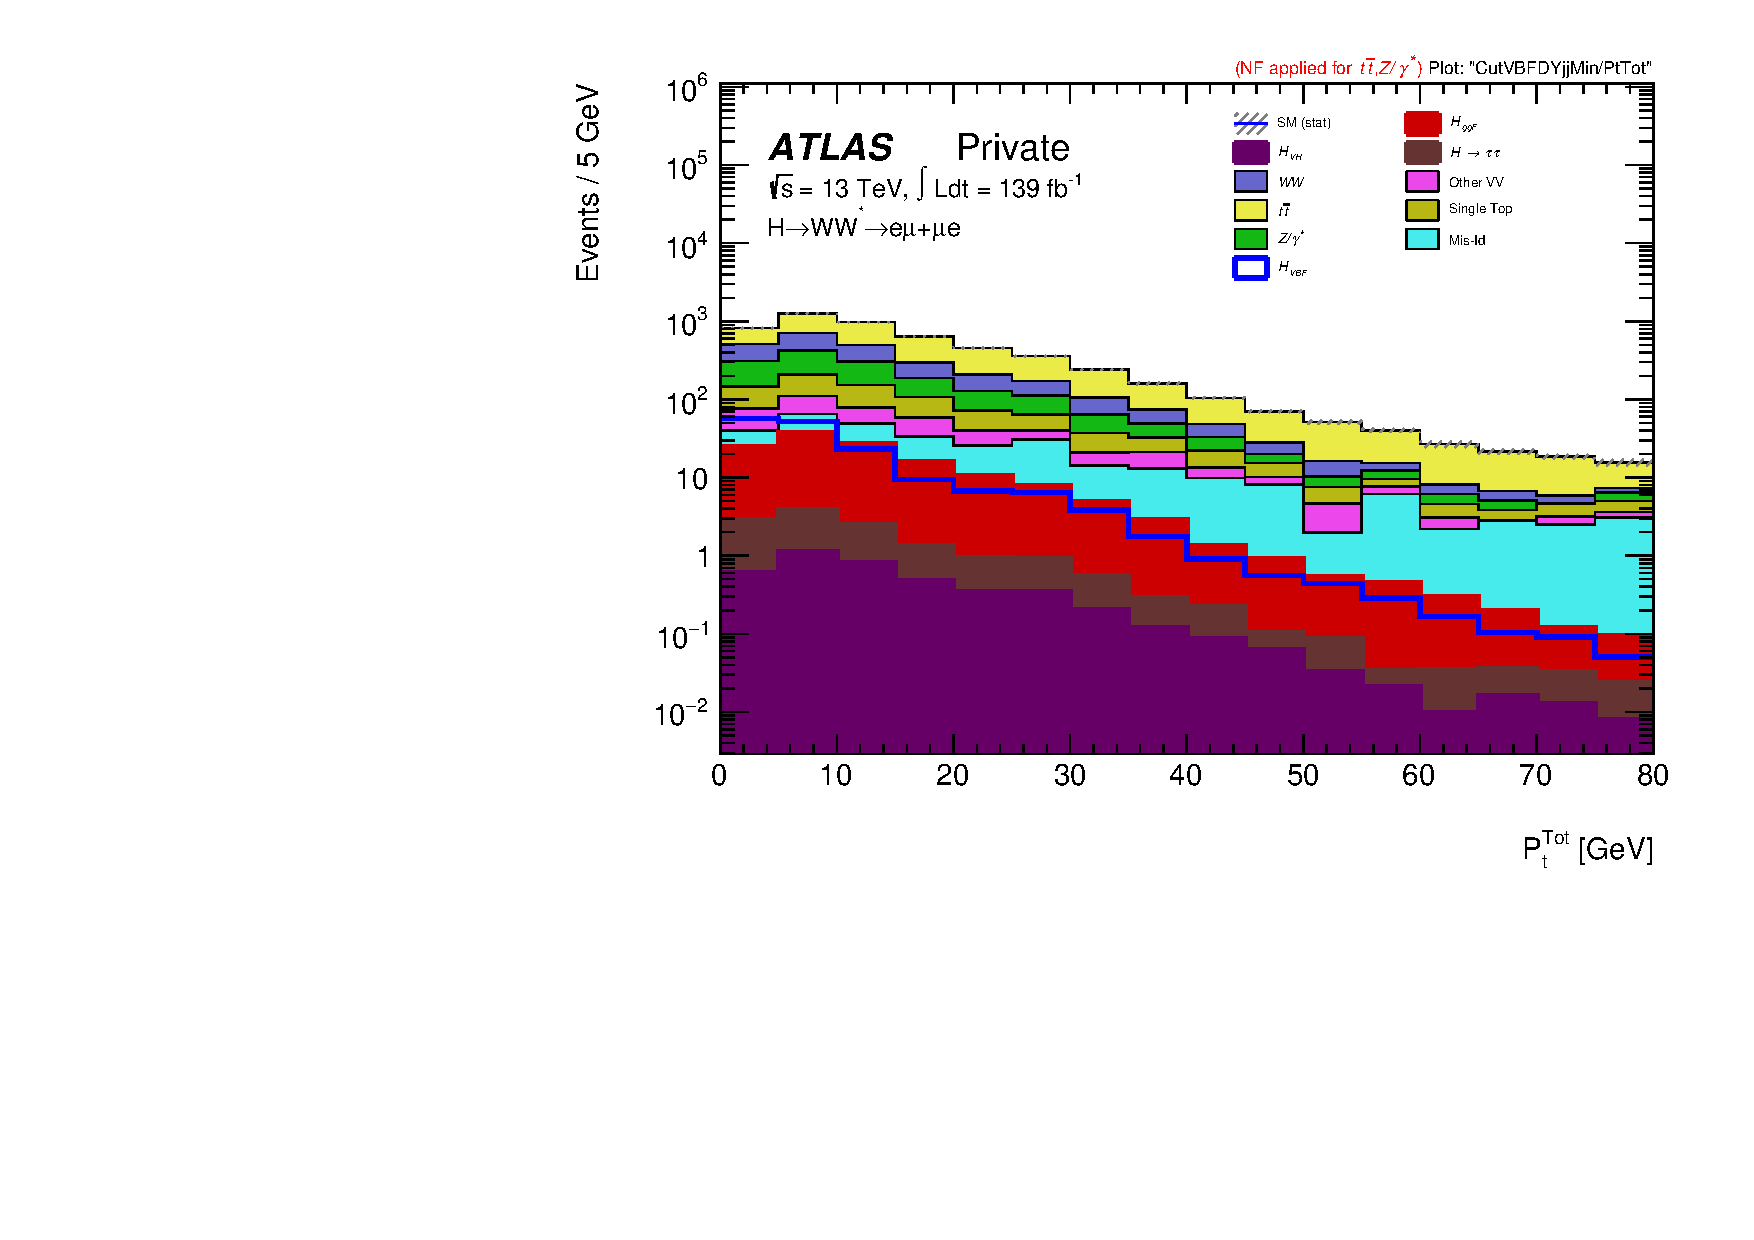
\includegraphics[width=0.3\textwidth]{Pictures/run2-emme-CutVBFDYjjMin-PtTot-log.pdf}
  }\hfill
  \subfloat[lep $p^T_{\text{lead}}$]{
      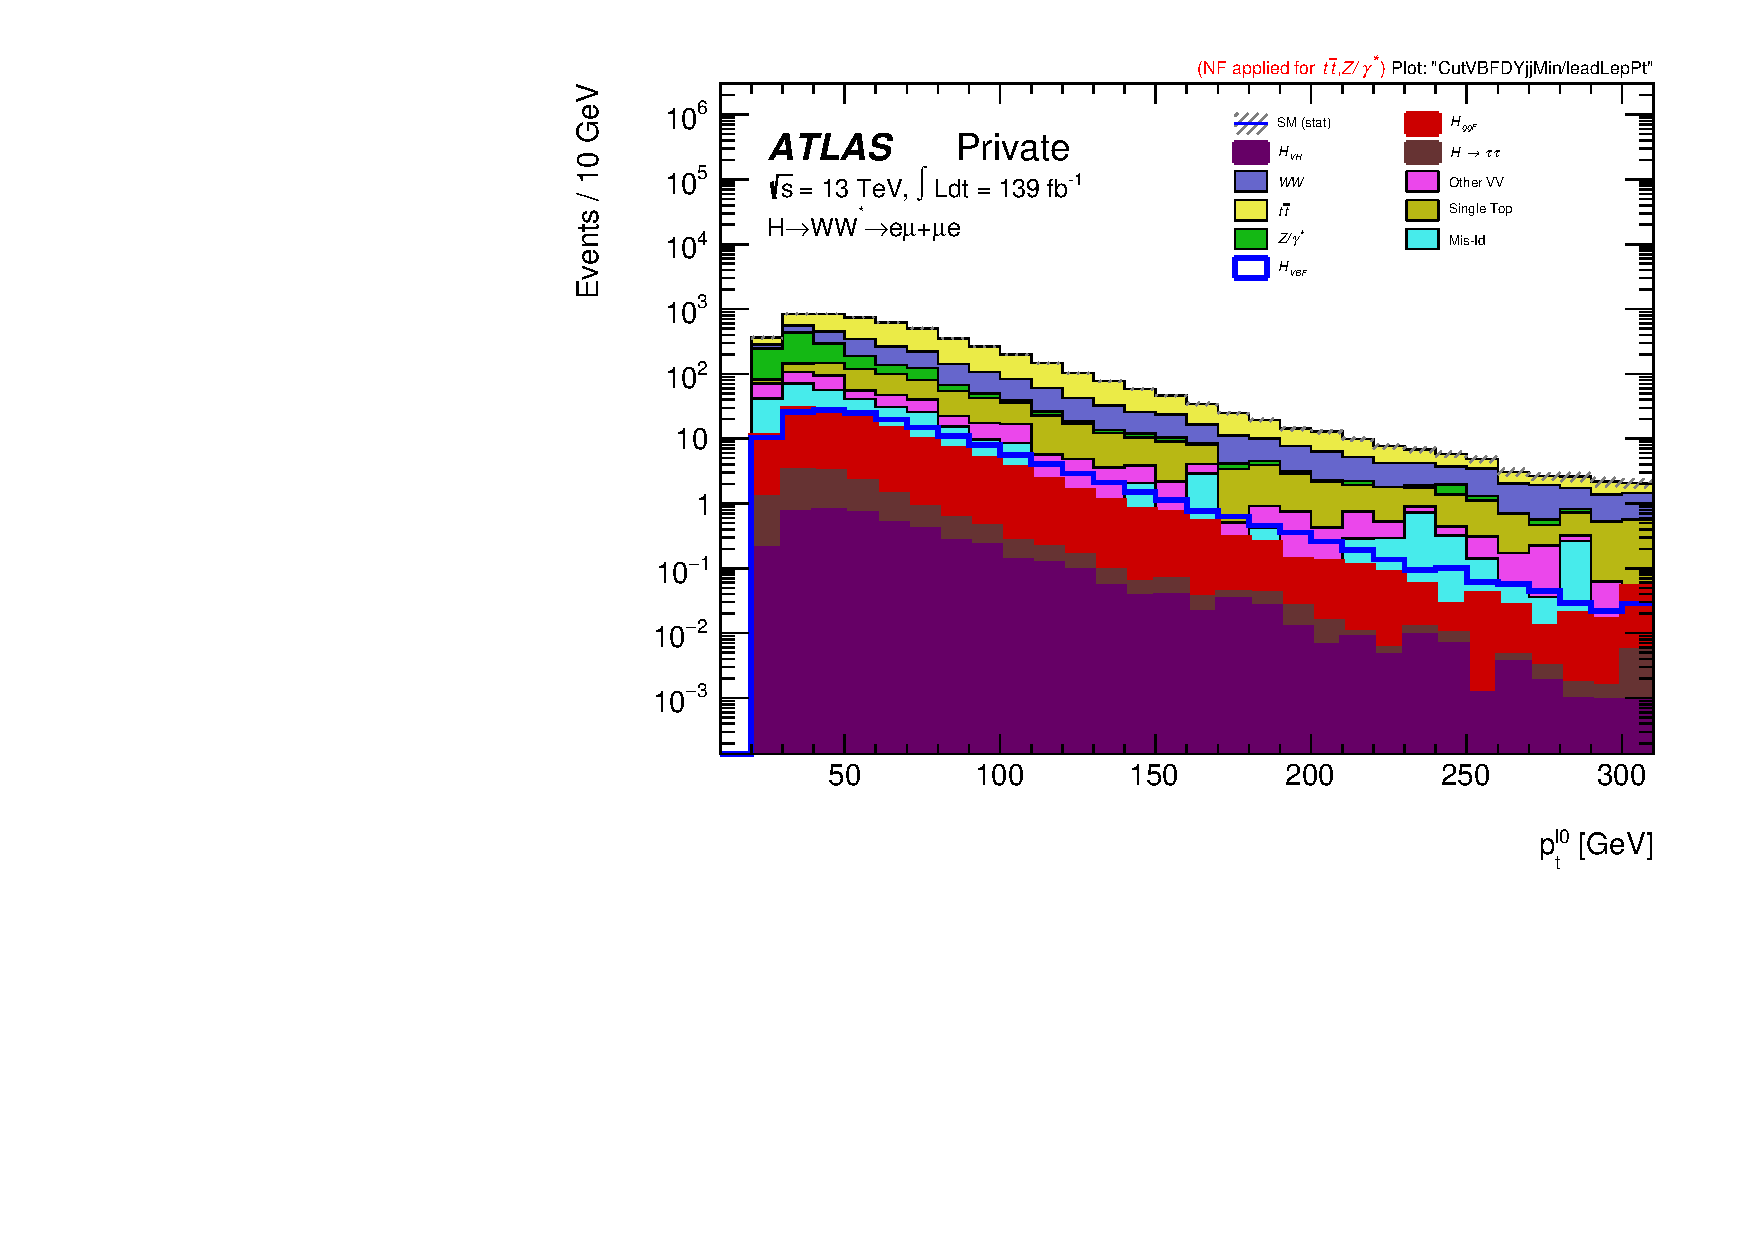
\includegraphics[width=0.3\textwidth]{Pictures/run2-emme-CutVBFDYjjMin-leadLepPt-log.pdf}
  }\hfill
  \subfloat[jet $p^T_{\text{lead}}$]{
      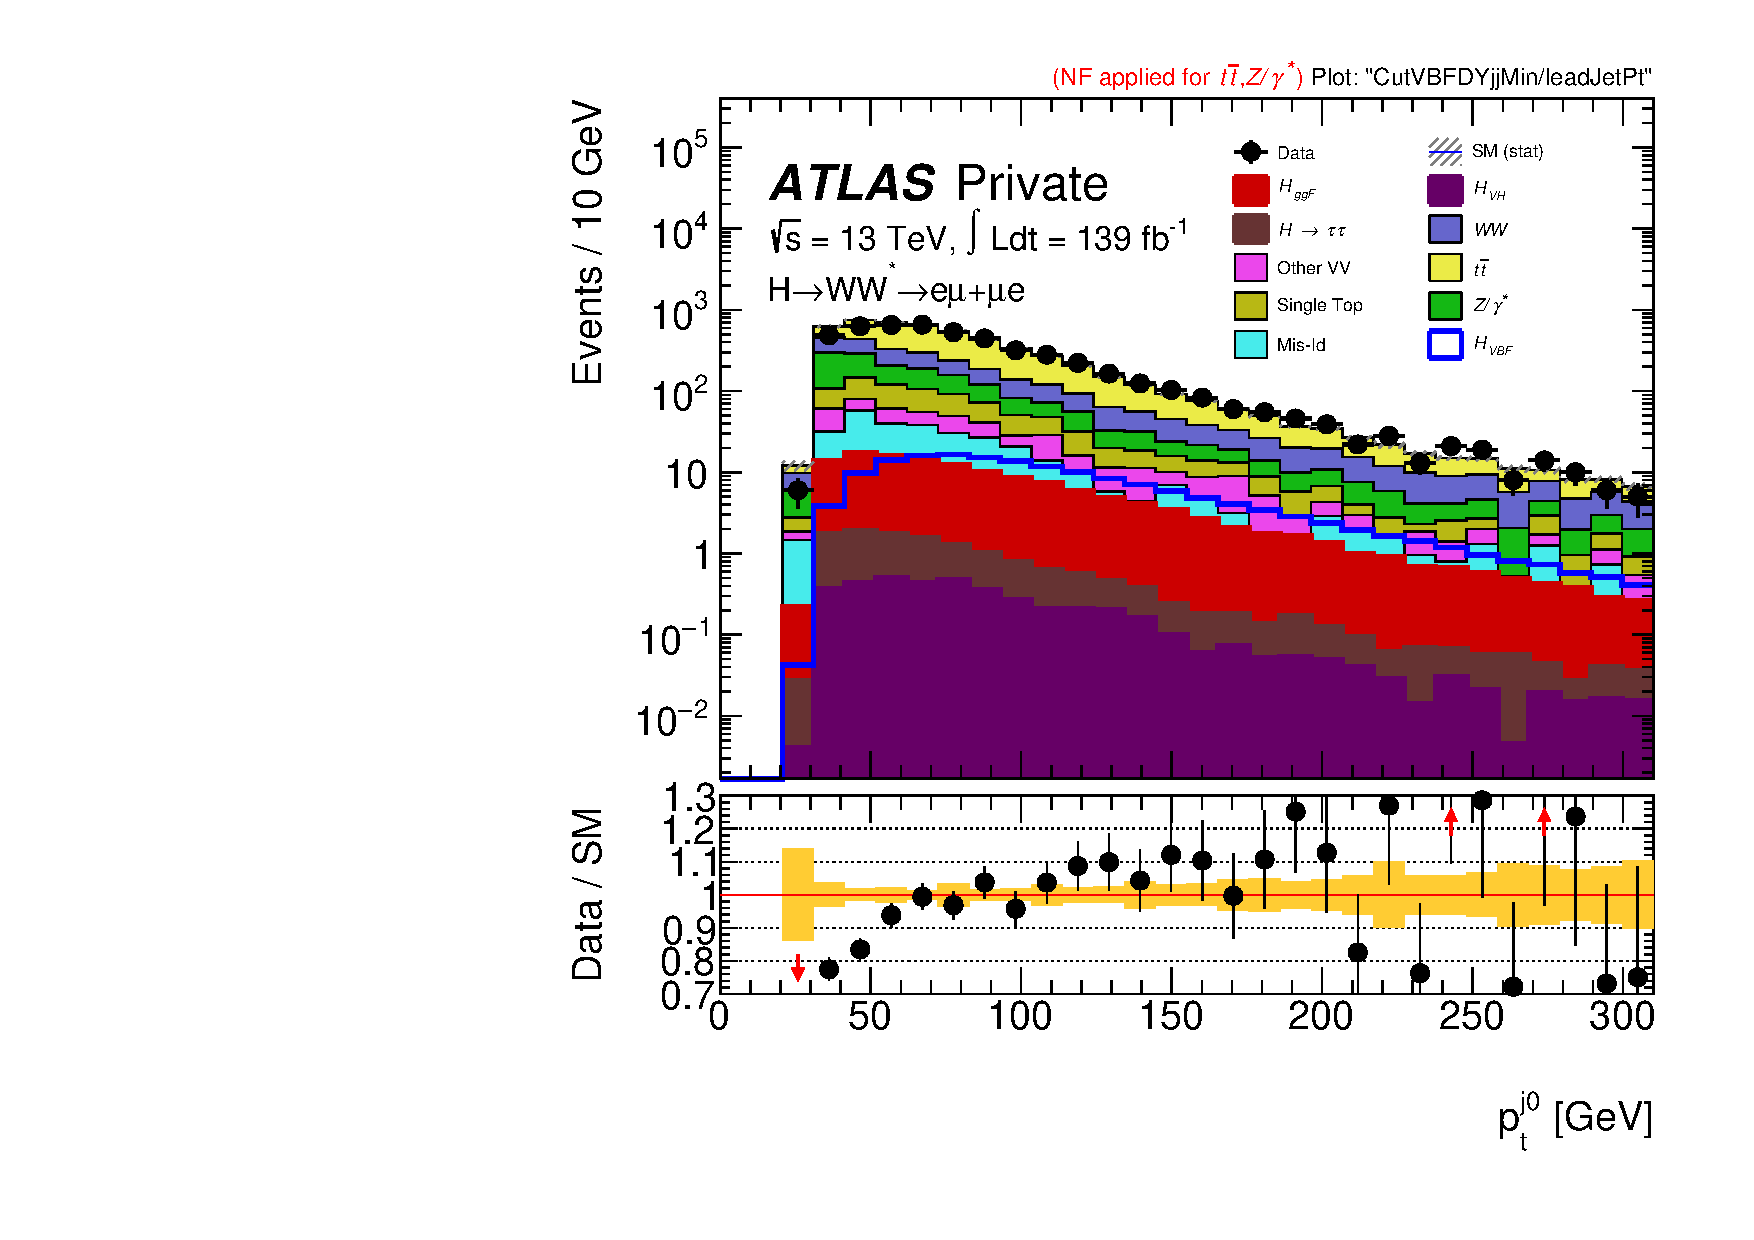
\includegraphics[width=0.3\textwidth]{Pictures/run2-emme-CutVBFDYjjMin-leadJetPt-log.pdf}
  }\hfill
%  \subfloat[lep $p^T_{\text{sublead}}$]{
%      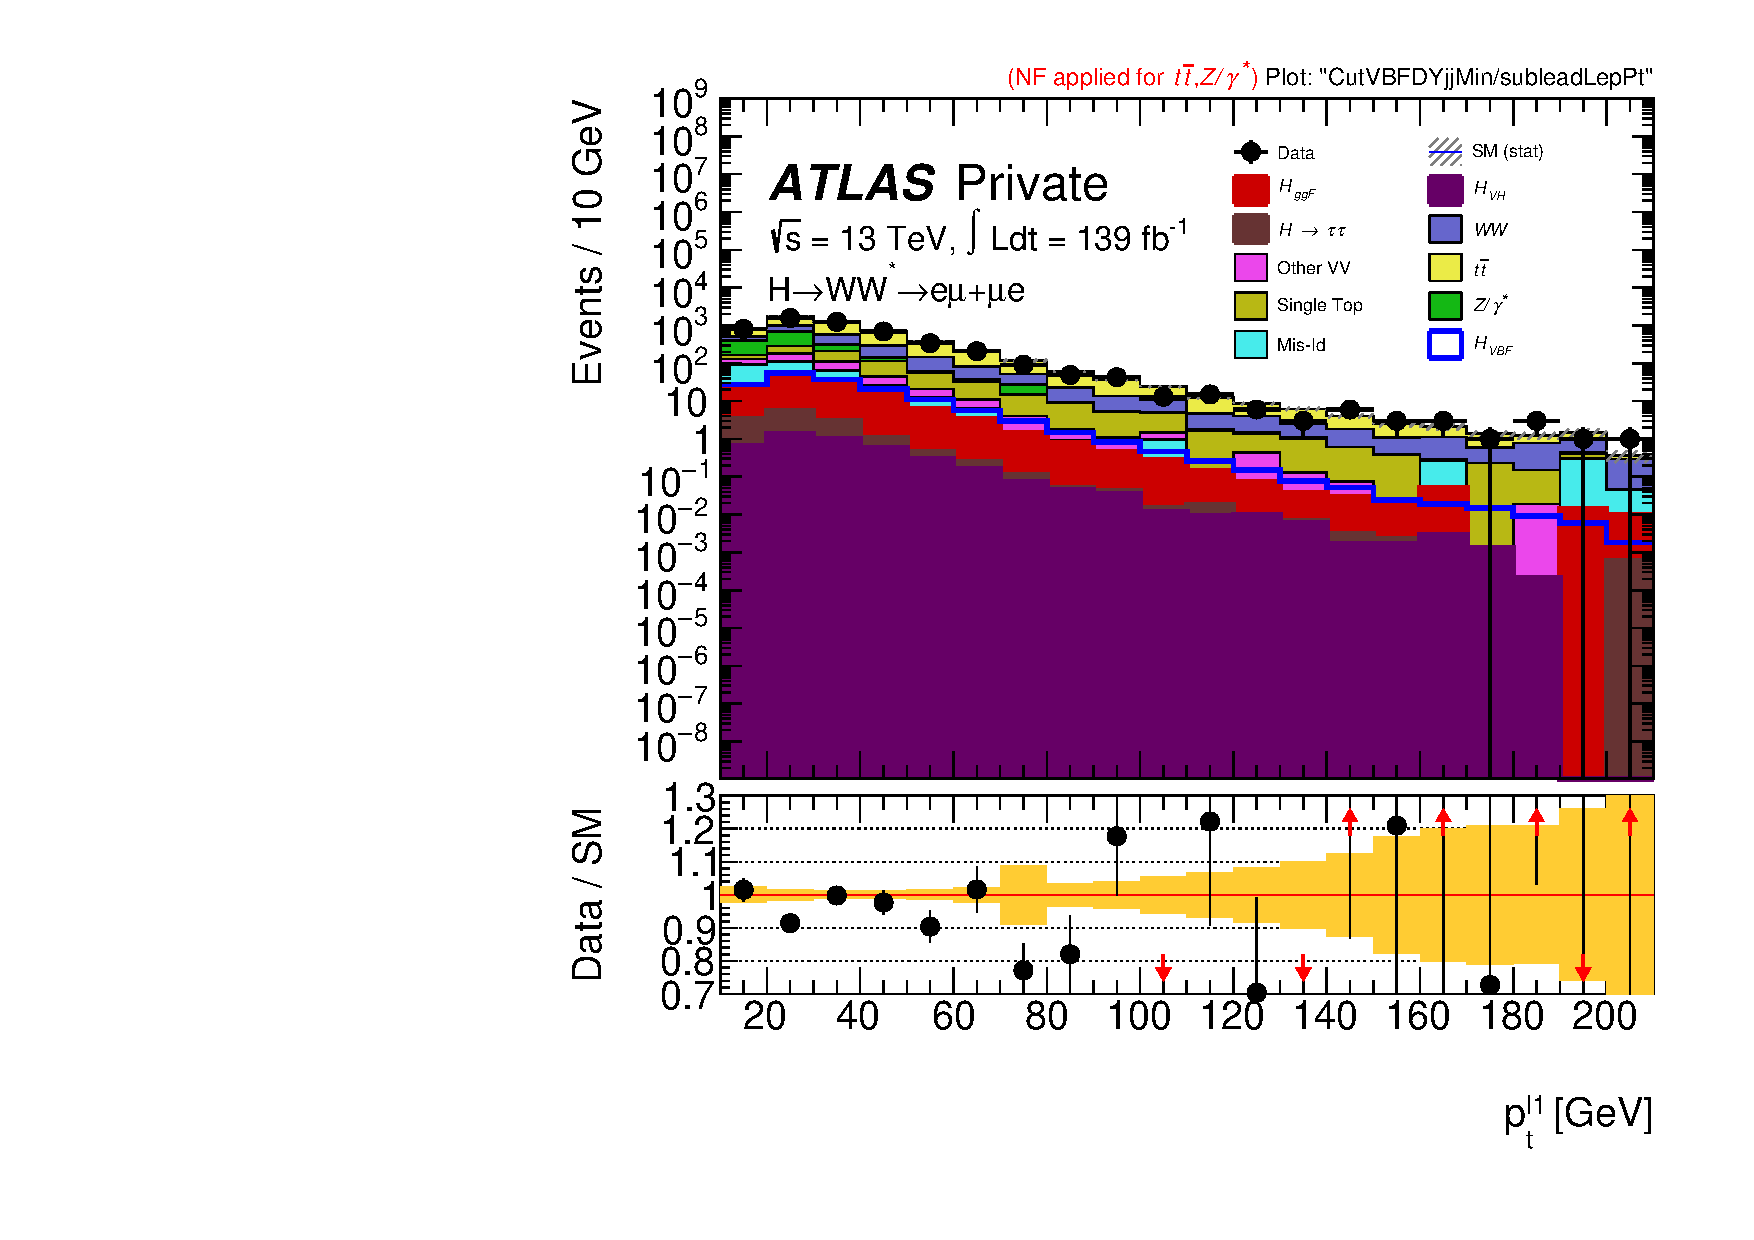
\includegraphics[width=0.3\textwidth]{Pictures/run2-emme-CutVBFDYjjMin-subleadLepPt-log.pdf}
%  }\hfill
%  \subfloat[jet $p^T_{\text{sublead}}$]{
%      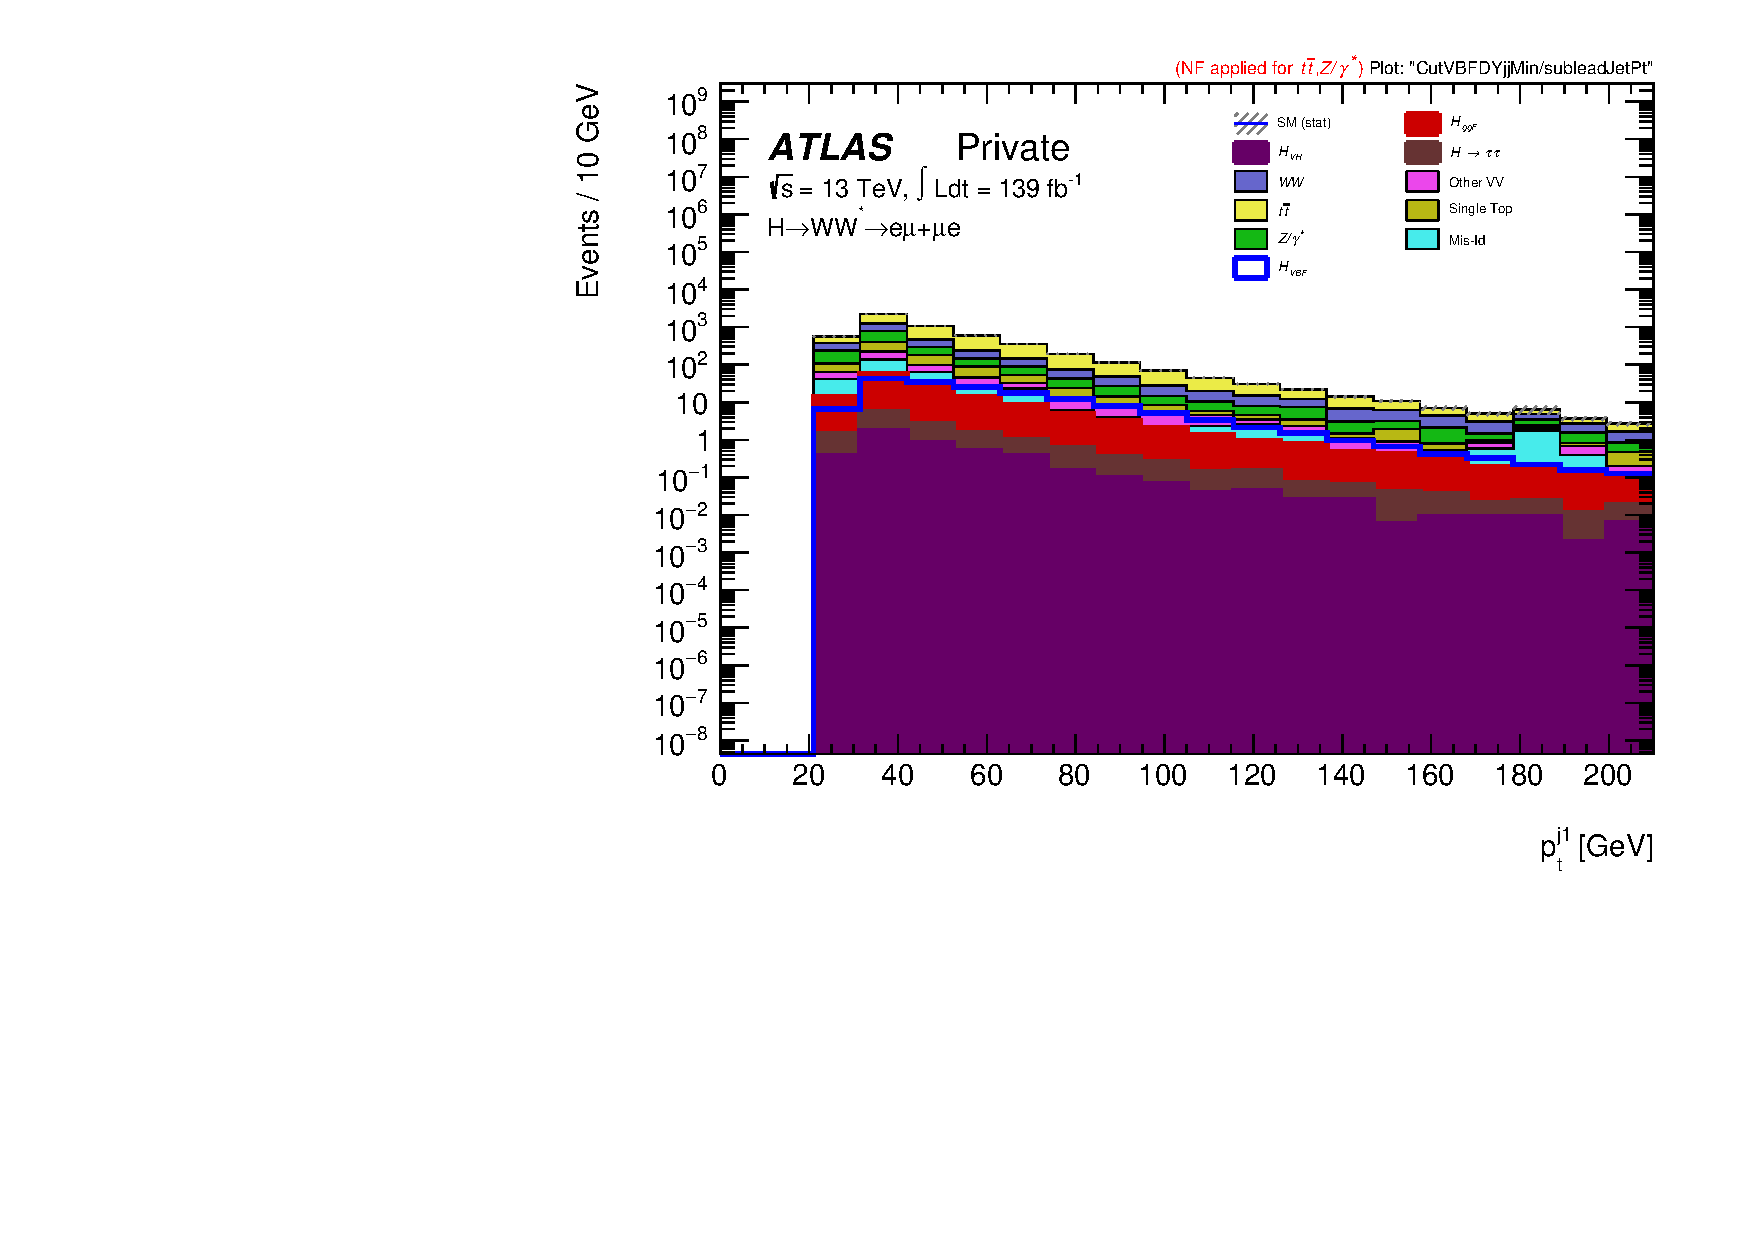
\includegraphics[width=0.3\textwidth]{Pictures/run2-emme-CutVBFDYjjMin-subleadJetPt-log.pdf}
%  }\hfill
%  \subfloat[$\Delta \Phi_{jj}$]{
%      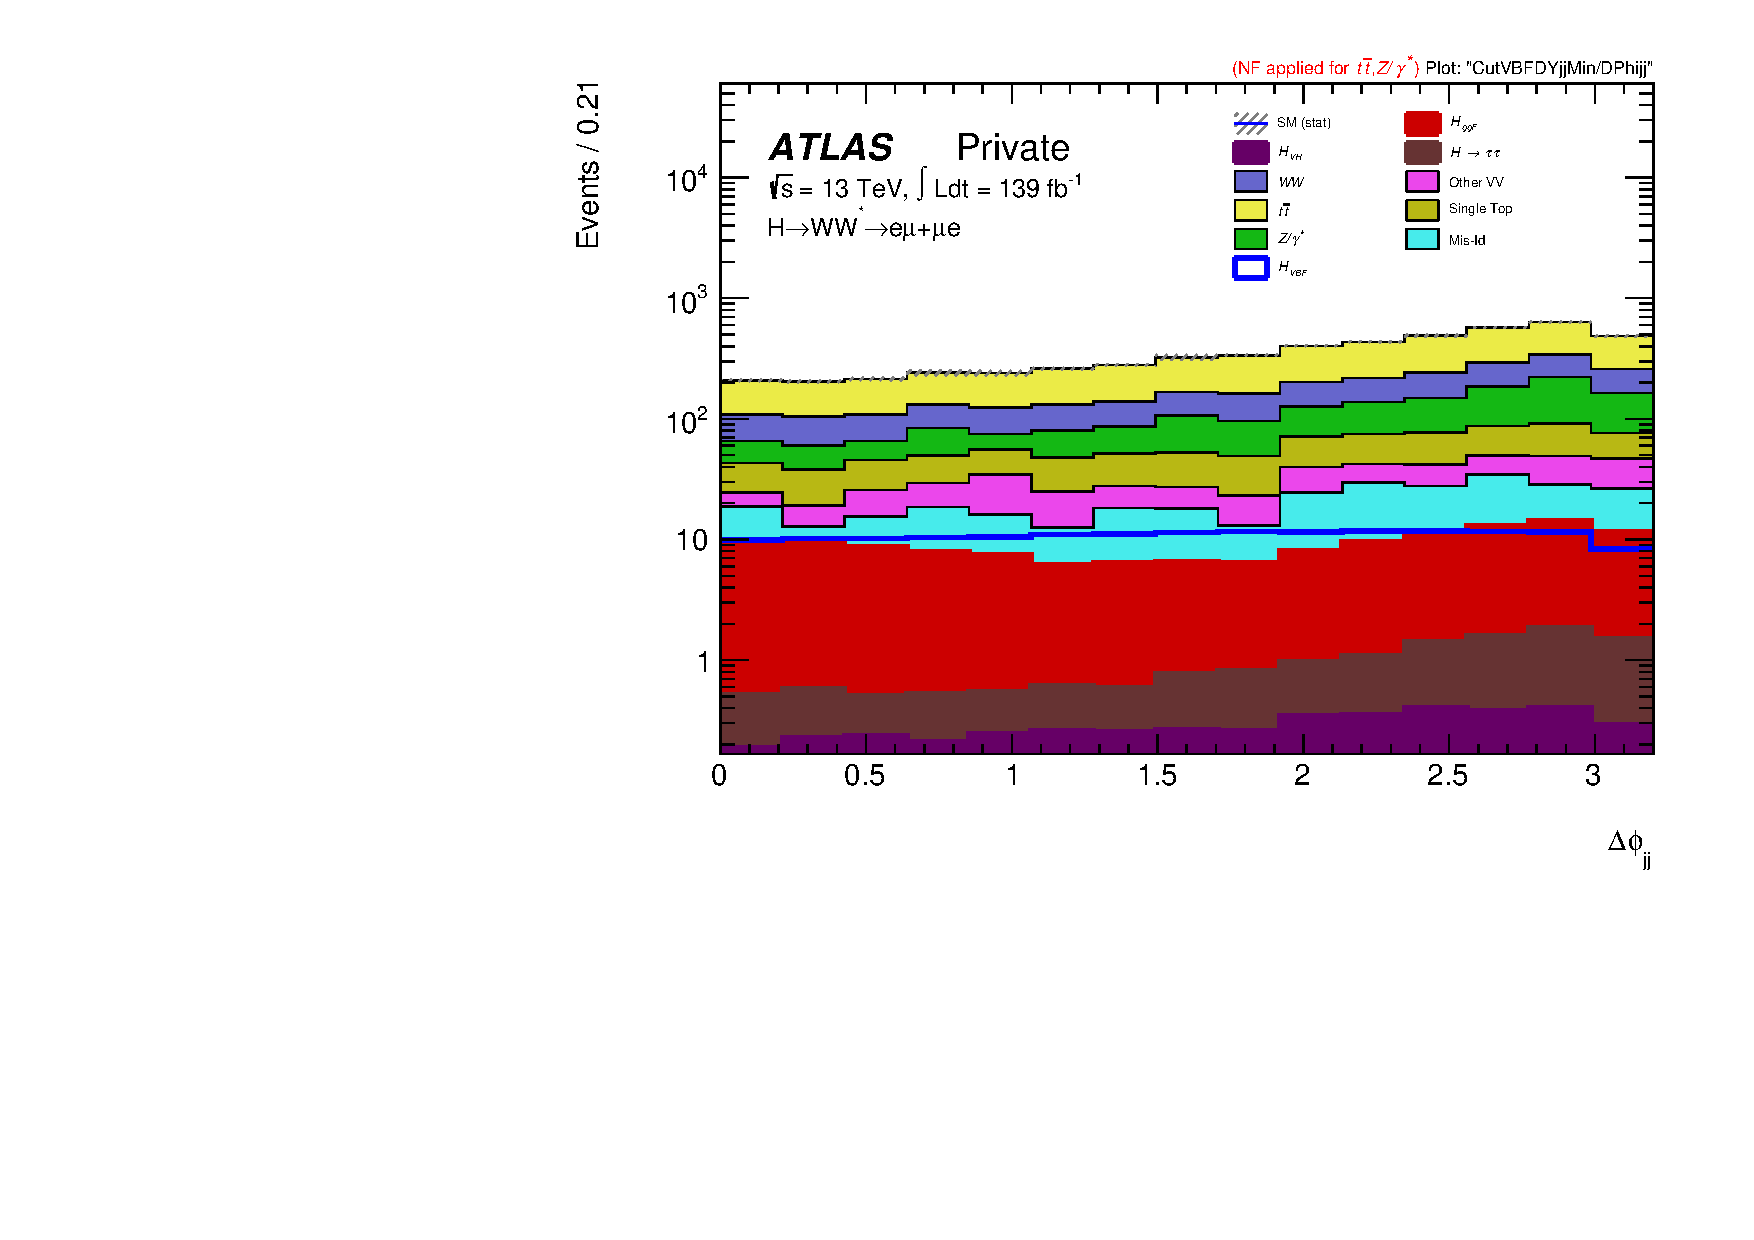
\includegraphics[width=0.3\textwidth]{Pictures/run2-emme-CutVBFDYjjMin-DPhijj-log.pdf}
%  }\hfill
  \subfloat[$\ensuremath{E_{\text{T,rel}}^{\text{miss}}}$]{
      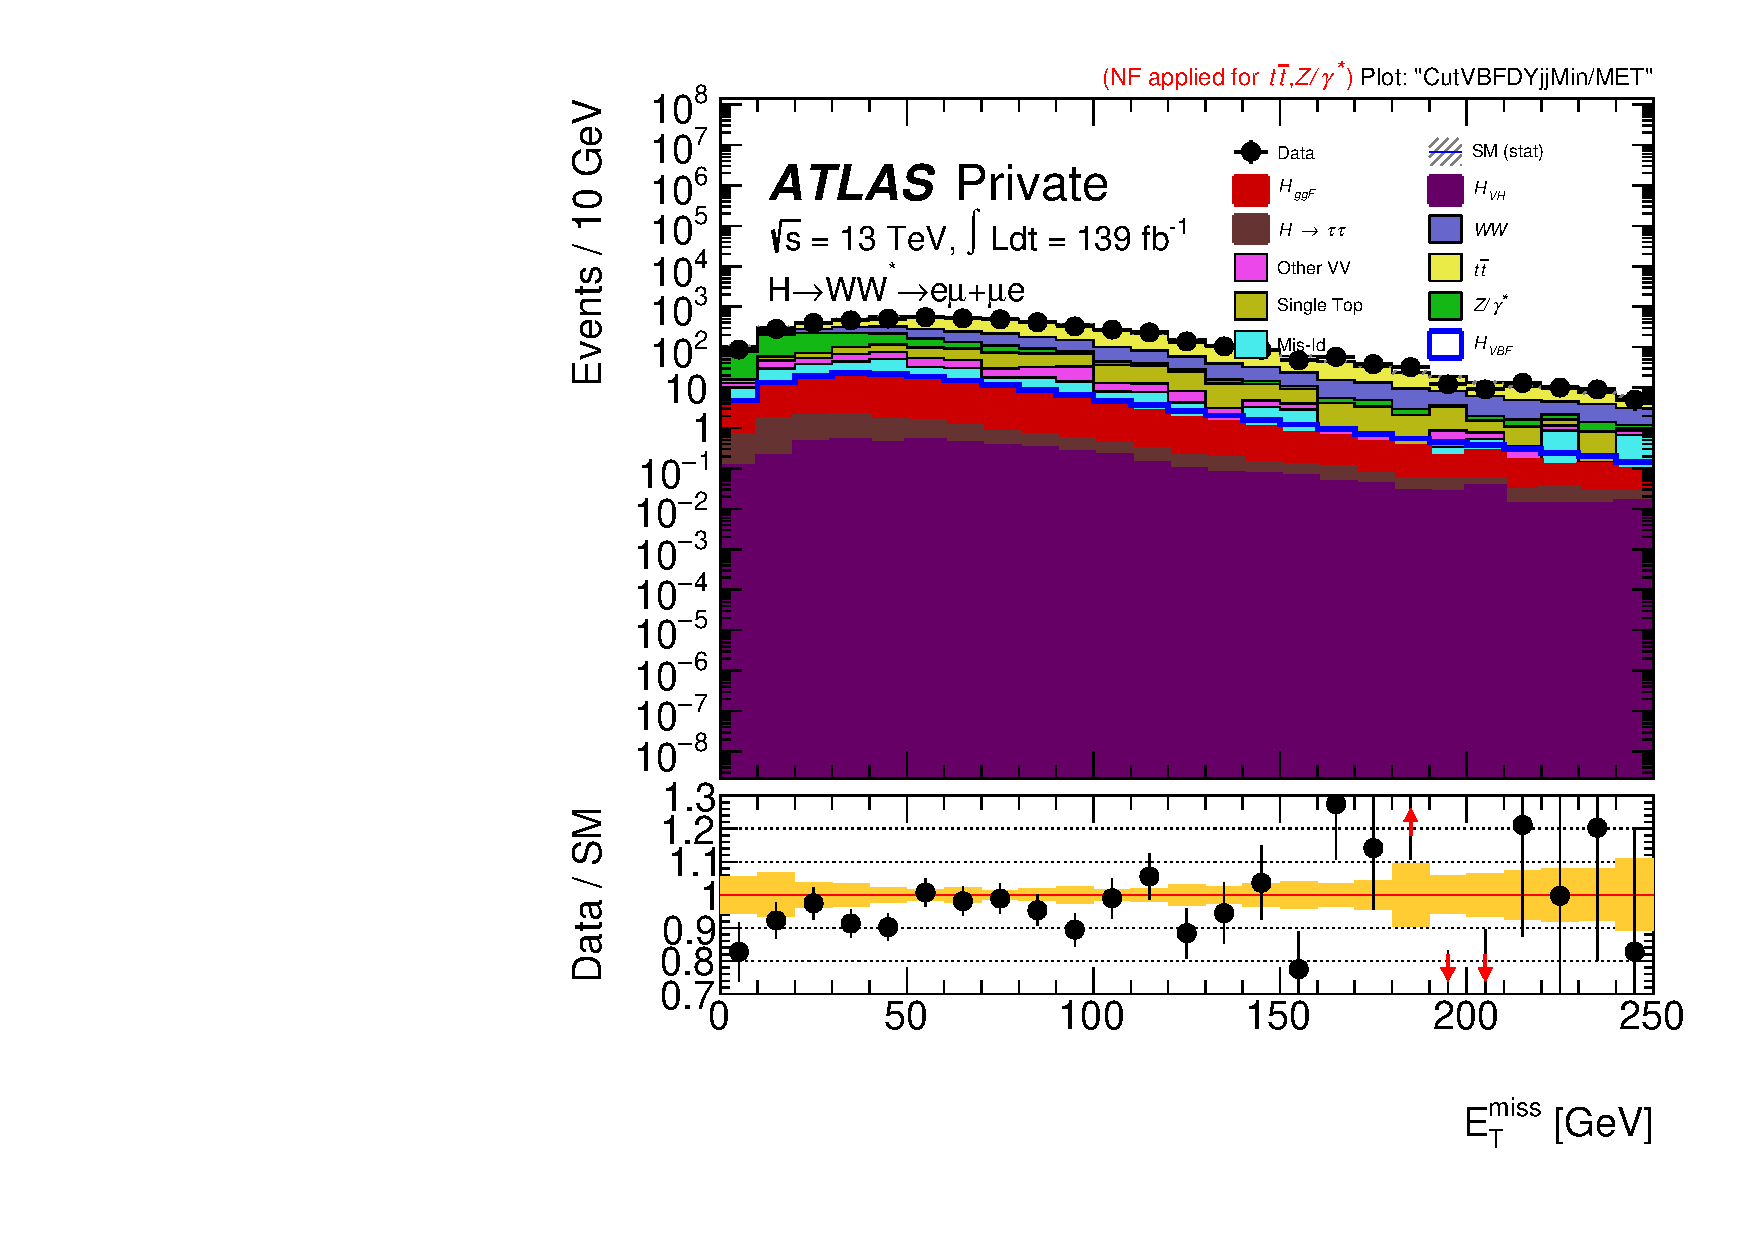
\includegraphics[width=0.3\textwidth]{Pictures/run2-emme-CutVBFDYjjMin-MET-log.pdf}
  }%\hfill
{\caption{Distributions of $\Delta Y_{\ell\ell}$, $\Delta \phi_{\ell\ell}$,$m_{\ell\ell}$,$m_T$,$p^T_{tot}$, lep $p^T_{\text{lead}}$, jet $p^T_{\text{lead}}$ and $\ensuremath{E_{\text{T,rel}}^{\text{miss}}}$ in the differential VBF signal region, many used as input to the BDT discriminating VBF from top $+WW$ backgrounds.
\label{fig:signalregion}}}
\end{figure}

\subsubsection{VBF signal boosted decision tree discriminant}
This analysis uses a number of boosted decision trees (BDTs) to both amplify our VBF signal and discriminate and reject a number of specific backgrounds. A decision tree is a collection of cuts designed to classify events as signal-like or background-like. A given signal event is correctly identified if it is placed in a signal-dominated leaf and vice-cersa for background events. After the initial tree is built, another tree is grown to better separate the signal and background events misidentified by the first tree. This proceeds iteratively until there is a collection of a specified number of trees, in a process known as boosting. A weighted average is taken from all these trees to form a BDT output discriminant with values ranging from -1 to 1.

This section will focus on the BDT trained and used in the signal region to isolate the VBF signal from dominant backgrounds (top and $WW$ events). The discriminant used in this analysis is the result of numerous studies on training parameters, input variables, and multivariate analysis techniques. Appendix C shows results from studies on using a multidimensional BDT to simultaneously discriminate VBF, ggF, and $WW$ background samples. While initially this 3D BDT showed promising results, estimation of ggF backgrounds through use of multiple control regions (summarized in the next chapter) showed better determination of the ggF background, so the one-dimensional method here was adopted. 

This BDT is trained using $e\mu+\mu e$ events after the VBF selection and the signal regions cuts including that on $n_{jets}$, $b$-veto, OLV, CJV, $M_{jj}$ and $\Delta Y_{jj}$. In this way, the phase space in which we train the BDT is exactly the same as the one where we apply it. The training includes only the top and $WW$ backgrounds and the VBF signal. Half of the available events are used for training and the other half are used to test the training. This corresponds to about 90,000 un-weighted $WW$ and top events and 100,000 raw VBF events. This training includes MC weights on events to best account for overall event distributions. There are approximately 2000 total weighted top and $WW$ events used in the training and 80 weighted VBF events. 
The TMVA BDTG interface is used to train and test the BDT~\cite{TMVA}. The optimal parameters were found through a scan of reasonable values and the final set is summarized in Table~\ref{tab:SRBDTparameters}.
\begin{table}[h!]
\centering
\begin{tabular}{|l|c|}
\hline
Parameter                                    & Value     \\
\hline
Boosting algorithm                           &  Gradient  \\
Maximum tree depth                           &  22       \\
Number of trees                              &  400     \\
Minimum number of events requires per mode   &  5\%      \\
Number of cuts                               &  7        \\
\hline
\end{tabular}
\caption{BDT parameters used for the VBF vs. top + $WW$ training.} 
\label{tab:SRBDTparameters}
\end{table}
This BDT utilizes 12 lepton and jet kinematic variables to distinguish between signal and background events. These include $\Delta Y_{jj}$, $\Delta Y_{\ell\ell}$, $\Delta \phi_{\ell\ell}$, $m_{jj}$, $m_{\ell\ell}$, $m_T$, $\eta_{j0}$, $\eta_{j1}$, $p^T_{j0}$, $p^T_{j1}$, $\Delta \phi_{jj}$, and $\sum$ centralities (L). While a larger variety of variables have been tested, these demonstrated the highest discrimination between VBF and top/$WW$ background. FIgures~\ref{fig:SRBDTinput} and \ref{fig:SRcorrSB} demonstrate the input distributions used to train the BDT and their correlations.
\begin{figure}[!htbp]
    \centering
    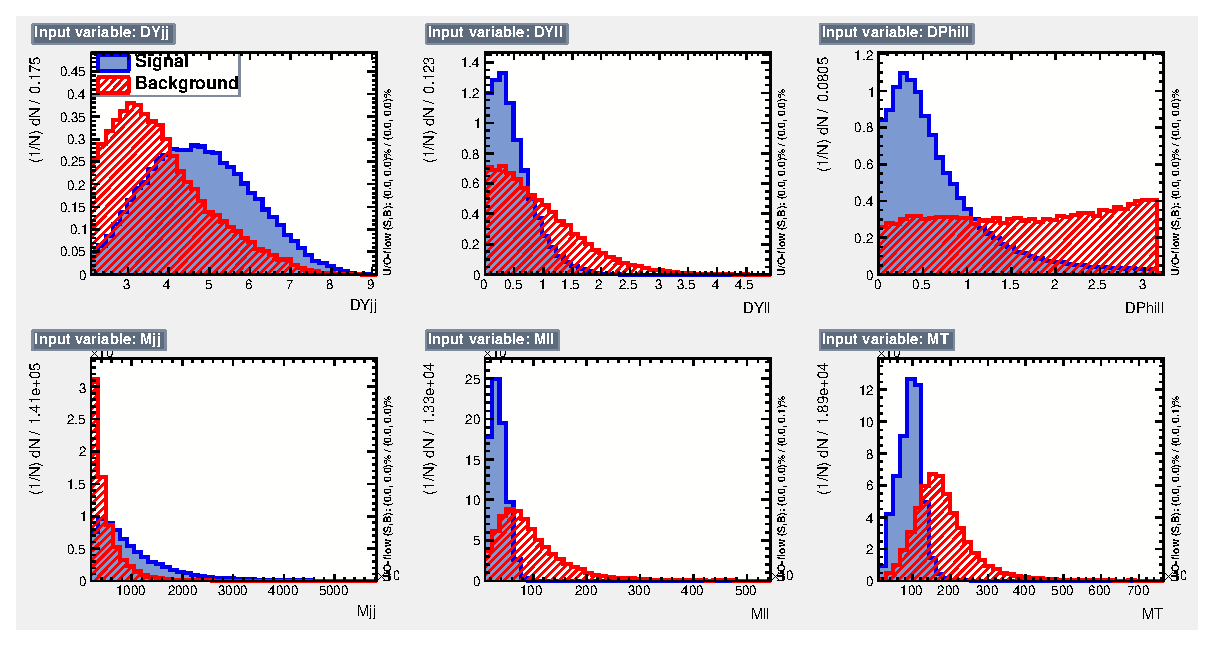
\includegraphics[width=0.7\linewidth]{Pictures/VBFvsWW+Top/variables_id_c1.eps}
    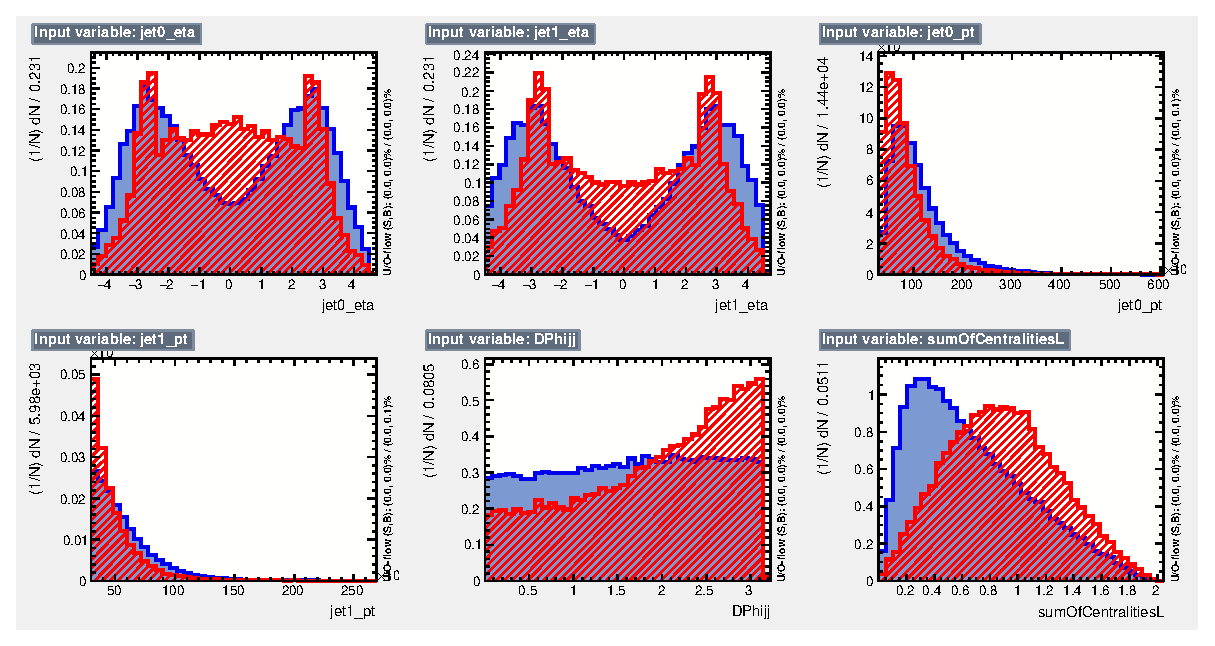
\includegraphics[width=0.7\linewidth]{Pictures/VBFvsWW+Top/variables_id_c2.eps}
    \caption{Distributions of input variables to VBF vs. top+$WW$ BDT. Samples are weighted and normalized to even numbers of background and signal events. Signal represents VBF and background top+$WW$~\cite{ourSupportNote}.}
    \label{fig:SRBDTinput}
\end{figure}

\begin{figure}[!htbp]
  \centering
  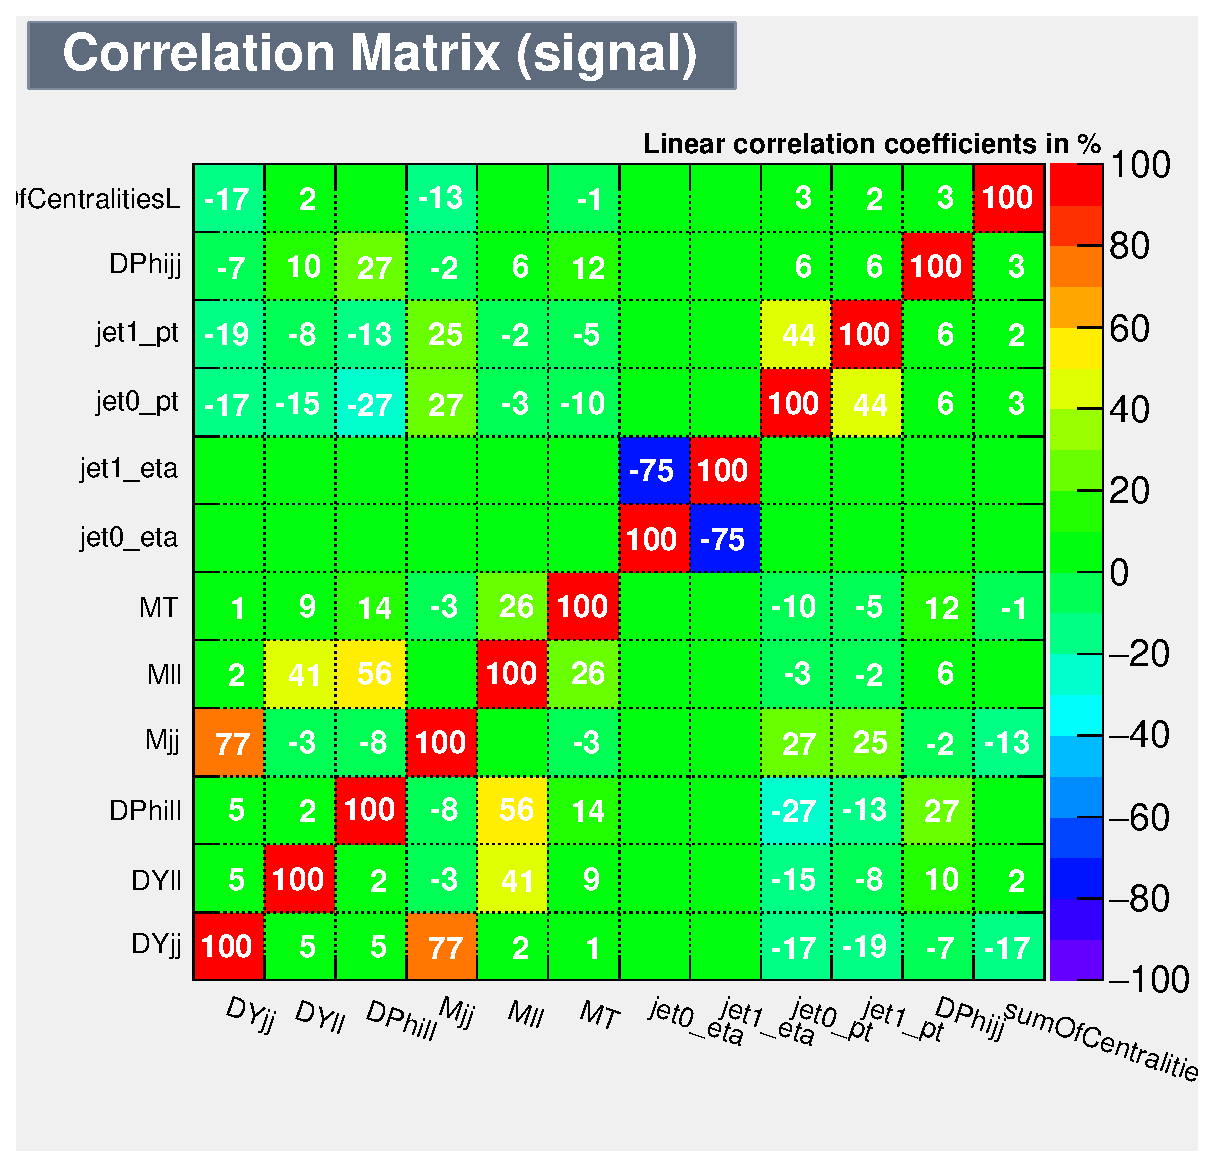
\includegraphics[width=.45\linewidth]{Pictures/VBFvsWW+Top/CorrelationMatrixS.eps}
  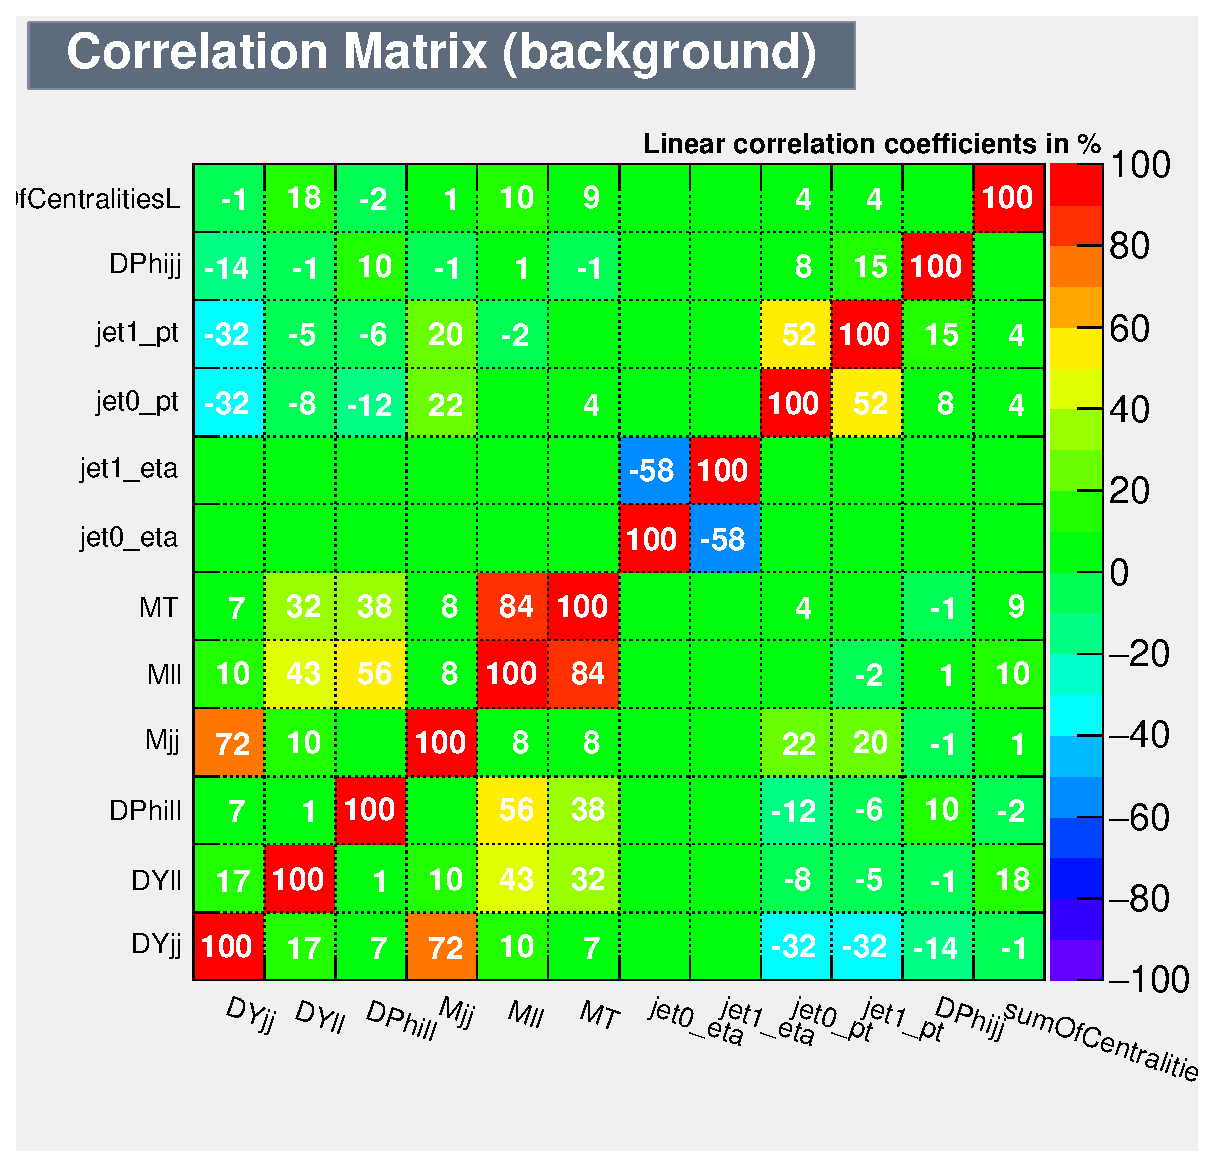
\includegraphics[width=.45\linewidth]{Pictures/VBFvsWW+Top/CorrelationMatrixB.eps}
\caption{Correlations of input variables to VBF vs. top +$WW$ BDT. Signal represents VBF and background top+$WW$~\cite{ourSupportNote}.}
\label{fig:SRcorrSB}
\end{figure}

The BDT training successfully separates VBF signal and top/$WW$ background. These backgrounds are considered together because our overall fit uses one parameter to estimate both $WW$ and top backgrounds due to their similar signatures. One useful metric to test the success of a classifier is a receiver operating characteristic curve (ROC curve). This curve measures signal acceptance over background rejection and its integral for a perfect classifier would be 1. In order to quantify the discrimination we use the integrated-ROC calculated through TMVA for weighted normalized samples and find an optimal value of 0.960, showing very good classification. Comparisons between the test and training show that the BDT is un-biased as one can see that the testing and trainings samples are quite similar. Differences between testing and training samples would imply overtraining, or the BDT using to many parameters on too few events. A Kolmogorov-Smirnov (KS) test is performed to measure if the two test and training distributions differ significantly. If the two distributions are random samples of the same parent distribution, the KS-test would give a uniformly distributed value between zero and one (or an average value of 0.5). The closer to 0.5 the KS-test value, the greater likelihood the curves come from the same parent, however this calculation is heavily skewed toward lower values so any value above zero (or not very close to zero, on order $10^{-4}$) can be considered not indicative of overtraining. For signal and background we find KS-test values of 0.107 and 0.154, and so no evidence of over-training. We can visualize the BDT output variable both on weighted normalized samples and on samples with all event weights applied. Figures~\ref{fig:SRBDTresult} and \ref{fig:SRBDTresult} show BDT results applied to normalized samples of VBF signal and top/$WW$ backgrounds and applied to all fully weighted samples in the signal region. 

\begin{figure}[!htbp]
\centering
  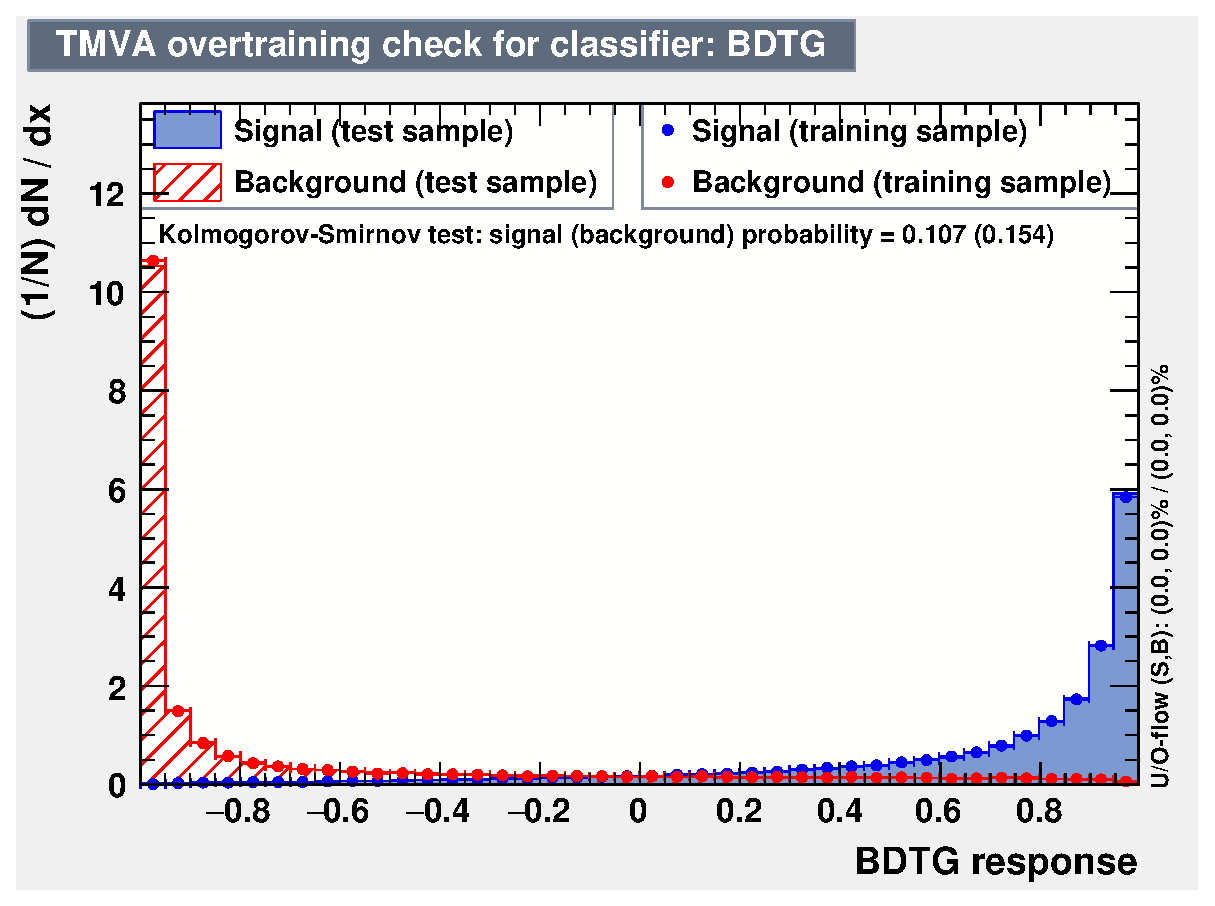
\includegraphics[width=.45\linewidth]{Pictures/VBFvsWW+Top/overtrain_BDTG.eps}
\caption{Weighted, normalized samples of VBF (signal) and top$+WW$ samples (background) plotted over BDT output distribution, overlaid testing and training samples shown~\cite{ourSupportNote}.}
\label{fig:SRBDTresult}
\end{figure}

\begin{figure}[!htbp]
\centering
  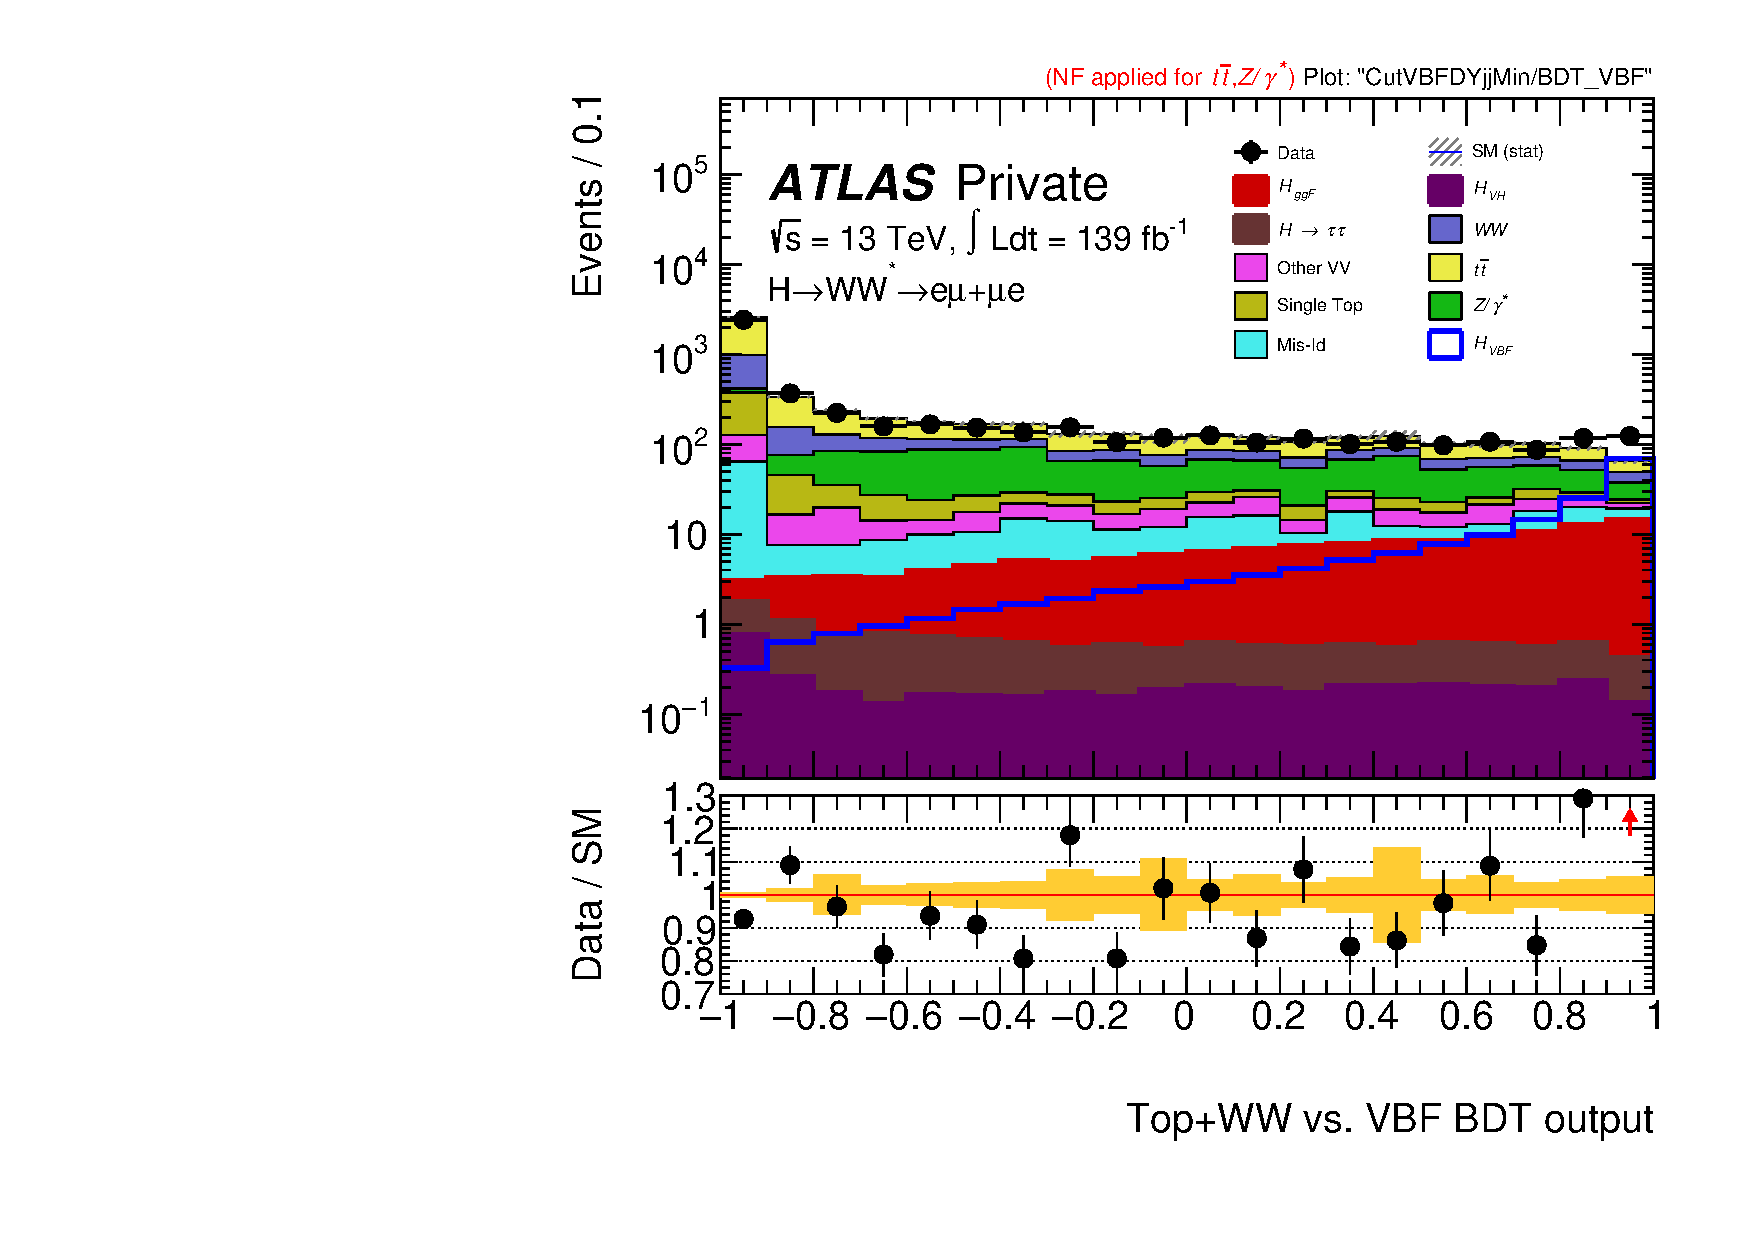
\includegraphics[width=.45\linewidth]{Pictures/run2-emme-CutVBFDYjjMin-BDT_VBF-log.pdf}
\caption{Full weighted samples of VBF signal and all backgrounds plotted over BDT output distribution after signal region selection.}
\label{fig:SRBDTresult2}
\end{figure}


We aim to fit this distribution in the signal region with high significance in uppermost bins of the distribution. Since this BDT is trained and applied in the signal region, we cannot directly test the modeling of input variables. However, these variables at the pre-selection level are shown earlier in the chapter and demonstrate successful modeling of data. The binning for this discriminant used in the statistical fit and its result are shown in the final chapter. 
